%%%%%%%%%%%%%%%%%%%%%%%%%%%%%%%%%%%%%%%%%%%%%%%%%%%%%%%%%%%%%%%
%% OXFORD THESIS TEMPLATE

% Use this template to produce a standard thesis that meets the Oxford University requirements for DPhil submission
%
% Originally by Keith A. Gillow (gillow@maths.ox.ac.uk), 1997
% Modified by Sam Evans (sam@samuelevansresearch.org), 2007
% Modified by John McManigle (john@oxfordechoes.com), 2015
%
% This version Copyright (c) 2015-2017 John McManigle
%
% Broad permissions are granted to use, modify, and distribute this software
% as specified in the MIT License included in this distribution's LICENSE file.
%

% I've (John) tried to comment this file extensively, so read through it to see how to use the various options.  Remember
% that in LaTeX, any line starting with a % is NOT executed.  Several places below, you have a choice of which line to use
% out of multiple options (eg draft vs final, for PDF vs for binding, etc.)  When you pick one, add a % to the beginning of
% the lines you don't want.


%%%%% CHOOSE PAGE LAYOUT
% The most common choices should be below.  You can also do other things, like replacing "a4paper" with "letterpaper", etc.

% This one will format for two-sided binding (ie left and right pages have mirror margins; blank pages inserted where needed):
\documentclass[a4paper,twoside]{ociamthesis}
% This one will format for one-sided binding (ie left margin > right margin; no extra blank pages):
%\documentclass[a4paper]{ociamthesis}
% This one will format for PDF output (ie equal margins, no extra blank pages):
%\documentclass[a4paper,nobind]{ociamthesis} 



%%%%% SELECT YOUR DRAFT OPTIONS
% Three options going on here; use in any combination.  But remember to turn the first two off before
% generating a PDF to send to the printer!

% This adds a "DRAFT" footer to every normal page.  (The first page of each chapter is not a "normal" page.)
\fancyfoot[C]{\emph{DRAFT Printed on \today}}  

% This highlights (in blue) corrections marked with (for words) \mccorrect{blah} or (for whole
% paragraphs) \begin{mccorrection} . . . \end{mccorrection}.  This can be useful for sending a PDF of
% your corrected thesis to your examiners for review.  Turn it off, and the blue disappears.
\correctionstrue


%%%%% BIBLIOGRAPHY SETUP
% Note that your bibliography will require some tweaking depending on your department, preferred format, etc.
% The options included below are just very basic "sciencey" and "humanitiesey" options to get started.
% If you've not used LaTeX before, I recommend reading a little about biblatex/biber and getting started with it.
% If you're already a LaTeX pro and are used to natbib or something, modify as necessary.
% Either way, you'll have to choose and configure an appropriate bibliography format...

% The science-type option: numerical in-text citation with references in order of appearance.
\usepackage[style=numeric-comp, sorting=none, backend=biber, doi=false, isbn=false, url=false]{biblatex}
\newcommand*{\bibtitle}{References}

% The humanities-type option: author-year in-text citation with an alphabetical works cited.
%\usepackage[style=authoryear, sorting=nyt, backend=biber, maxcitenames=2, useprefix, doi=false, isbn=false]{biblatex}
%\newcommand*{\bibtitle}{Works Cited}

% This makes the bibliography left-aligned (not 'justified') and slightly smaller font.
\renewcommand*{\bibfont}{\raggedright\small}

% Change this to the name of your .bib file (usually exported from a citation manager like Zotero or EndNote).
\addbibresource{references.bib}


% Uncomment this if you want equation numbers per section (2.3.12), instead of per chapter (2.18):
%\numberwithin{equation}{subsection}



%%%%% THESIS / TITLE PAGE INFORMATION
% Everybody needs to complete the following:
\title{Rings and Things}
\author{David Ormrod Morley}
\college{Balliol College}

% Master's candidates who require the alternate title page (with candidate number and word count)
% must also un-comment and complete the following three lines:
%\masterssubmissiontrue
%\candidateno{933516}
%\wordcount{28,815}

% Uncomment the following line if your degree also includes exams (eg most masters):
%\renewcommand{\submittedtext}{Submitted in partial completion of the}
% Your full degree name.  (But remember that DPhils aren't "in" anything.  They're just DPhils.)
\degree{Doctor of Philosophy}
% Term and year of submission, or date if your board requires (eg most masters)
\degreedate{Trinity 2020}


%%%%% YOUR OWN PERSONAL MACROS
% This is a good place to dump your own LaTeX macros as they come up.

% To make text superscripts shortcuts
	\renewcommand{\th}{\textsuperscript{th}} % ex: I won 4\th place
	\newcommand{\nd}{\textsuperscript{nd}}
	\renewcommand{\st}{\textsuperscript{st}}
	\newcommand{\rd}{\textsuperscript{rd}}

%%%%% THE ACTUAL DOCUMENT STARTS HERE
\begin{document}



%%%%% CHOOSE YOUR LINE SPACING HERE
% This is the official option.  Use it for your submission copy and library copy:
\setlength{\textbaselineskip}{22pt plus2pt}
% This is closer spacing (about 1.5-spaced) that you might prefer for your personal copies:
%\setlength{\textbaselineskip}{18pt plus2pt minus1pt}

% You can set the spacing here for the roman-numbered pages (acknowledgements, table of contents, etc.)
\setlength{\frontmatterbaselineskip}{17pt plus1pt minus1pt}

% Leave this line alone; it gets things started for the real document.
\setlength{\baselineskip}{\textbaselineskip}


%%%%% CHOOSE YOUR SECTION NUMBERING DEPTH HERE
% You have two choices.  First, how far down are sections numbered?  (Below that, they're named but
% don't get numbers.)  Second, what level of section appears in the table of contents?  These don't have
% to match: you can have numbered sections that don't show up in the ToC, or unnumbered sections that
% do.  Throughout, 0 = chapter; 1 = section; 2 = subsection; 3 = subsubsection, 4 = paragraph...

% The level that gets a number:
\setcounter{secnumdepth}{2}
% The level that shows up in the ToC:
\setcounter{tocdepth}{2}


%%%%% ABSTRACT SEPARATE
% This is used to create the separate, one-page abstract that you are required to hand into the Exam
% Schools.  You can comment it out to generate a PDF for printing or whatnot.
%\begin{abstractseparate}
%	Investigations into \td{} network\--forming materials have renewed importance due to the experimental synthesis of ultra\--thin films of carbon, silica and aluminosilicate glasses.
Microscopy on the disordered phases of these materials reveals a percolating ring structure, identifying them as candidates for range of technologically useful materials, with applications including catalysis and gas separation.
The ability to characterise, understand and control the structure of the pore landscape in such materials is therefore central to their further development.

The overall aim of this thesis is to improve the simulation and characterisation of \td{} disordered materials.
The key is to accurately quantify and reproduce the ring structure, described by the ring size distribution and ring\--ring correlations.
This will be achieved by relating previous empirical laws (namely \lm's law and the \aw{} law), to well\--defined metrics in network science, and developing a variety of \mc{} methods to generate networks with controllable ring structure and topologies.

The first of these methods will be a sequential growth algorithm to construct triangle rafts (a proxy for silica bilayers), which will be shown to produce configurations commensurate with those from experiment.
Following from this, a modified bond switching algorithm will be used to investigate more generic systems, spanning a variety of atomic coordination environments, potential models and topologies. 
Fundamental relationships between these measures and the ring structure will be demonstrated by systematically varying the system parameters.
In addition, hard particle \mc{} techniques will be used to generate Voronoi diagrams, making contact with experimental studies on quasi\--\td{} colloidal systems.

Treating these diverse physical systems as complex networks allows a generalised network theory to be developed.
Traditional ring measures will be related to well\--defined metrics from network theory, namely the node degree distribution and the assortativity.
This will enable seemingly disparate physical systems to be compared and ties them into the wider field of network science.

Further applications of this work to real systems will be illustrated with analyses on a range of experimental (or experimentally motivated) data.
The appropriateness of weighted and unweighted Voronoi constructions will be evaluated for colloidal monolayers.
The ring structure of procrystalline lattices will be demonstrated to be related to the underlying parent lattice and atomic coordination environments.
Finally, a tool from topological data analysis, termed persistent homology, will be investigated and shown to be a potential complement to more traditional measures of structural disorder.

%\textbf{Keywords}: Network theory, Monte Carlo methods, silica bilayers, colloidal monolayers, procrystalline lattices, Voronoi diagrams, persistent homology
 % Create an abstract.tex file in the 'text' folder for your abstract.
%\end{abstractseparate}


% JEM: Pages are roman numbered from here, though page numbers are invisible until ToC.  This is in
% keeping with most typesetting conventions.
\begin{romanpages}

% Title page is created here
\maketitle

%%%%% DEDICATION -- If you'd like one, un-comment the following.
%\begin{dedication}
%This thesis is dedicated to\\
%someone\\
%for some special reason\\
%\end{dedication}

%%%%% ACKNOWLEDGEMENTS -- Nothing to do here except comment out if you don't want it.
%\begin{acknowledgements}
% 	%\subsection*{Personal}

So long, and thanks for all the fish.

%\subsection*{Institutional}

%If you want to separate out your thanks for funding and institutional support, I don't think there's any rule against it.  Of course, you could also just remove the subsections and do one big traditional acknowledgement section.

%\end{acknowledgements}

%%%%% ABSTRACT -- Nothing to do here except comment out if you don't want it.
%\begin{abstract}
%	Investigations into \td{} network\--forming materials have renewed importance due to the experimental synthesis of ultra\--thin films of carbon, silica and aluminosilicate glasses.
Microscopy on the disordered phases of these materials reveals a percolating ring structure, identifying them as candidates for range of technologically useful materials, with applications including catalysis and gas separation.
The ability to characterise, understand and control the structure of the pore landscape in such materials is therefore central to their further development.

The overall aim of this thesis is to improve the simulation and characterisation of \td{} disordered materials.
The key is to accurately quantify and reproduce the ring structure, described by the ring size distribution and ring\--ring correlations.
This will be achieved by relating previous empirical laws (namely \lm's law and the \aw{} law), to well\--defined metrics in network science, and developing a variety of \mc{} methods to generate networks with controllable ring structure and topologies.

The first of these methods will be a sequential growth algorithm to construct triangle rafts (a proxy for silica bilayers), which will be shown to produce configurations commensurate with those from experiment.
Following from this, a modified bond switching algorithm will be used to investigate more generic systems, spanning a variety of atomic coordination environments, potential models and topologies. 
Fundamental relationships between these measures and the ring structure will be demonstrated by systematically varying the system parameters.
In addition, hard particle \mc{} techniques will be used to generate Voronoi diagrams, making contact with experimental studies on quasi\--\td{} colloidal systems.

Treating these diverse physical systems as complex networks allows a generalised network theory to be developed.
Traditional ring measures will be related to well\--defined metrics from network theory, namely the node degree distribution and the assortativity.
This will enable seemingly disparate physical systems to be compared and ties them into the wider field of network science.

Further applications of this work to real systems will be illustrated with analyses on a range of experimental (or experimentally motivated) data.
The appropriateness of weighted and unweighted Voronoi constructions will be evaluated for colloidal monolayers.
The ring structure of procrystalline lattices will be demonstrated to be related to the underlying parent lattice and atomic coordination environments.
Finally, a tool from topological data analysis, termed persistent homology, will be investigated and shown to be a potential complement to more traditional measures of structural disorder.

%\textbf{Keywords}: Network theory, Monte Carlo methods, silica bilayers, colloidal monolayers, procrystalline lattices, Voronoi diagrams, persistent homology

%\end{abstract}

%%%%% MINI TABLES
% This lays the groundwork for per-chapter, mini tables of contents.  Comment the following line
% (and remove \minitoc from the chapter files) if you don't want this.  Un-comment either of the
% next two lines if you want a per-chapter list of figures or tables.
%\dominitoc % include a mini table of contents
%\dominilof  % include a mini list of figures
%\dominilot  % include a mini list of tables

% This aligns the bottom of the text of each page.  It generally makes things look better.
\flushbottom

% This is where the whole-document ToC appears:
\tableofcontents

% DOM
\clearpage
\listofdavidnote
\listofmarknote

%\listoffigures
%	\mtcaddchapter
% \mtcaddchapter is needed when adding a non-chapter (but chapter-like) entity to avoid confusing minitoc

% Uncomment to generate a list of tables:
%\listoftables
%	\mtcaddchapter

%%%%% LIST OF ABBREVIATIONS
% This example includes a list of abbreviations.  Look at text/abbreviations.tex to see how that file is
% formatted.  The template can handle any kind of list though, so this might be a good place for a
% glossary, etc.
%% First parameter can be changed eg to "Glossary" or something.
% Second parameter is the max length of bold terms.
\begin{mclistof}{List of Abbreviations}{3.2cm}

\item[2D, 3D] Two- or three- dimensional.

\end{mclistof} 

%The work presented in this thesis has led to the following publications:

\begin{itemize}

	\item \textbf{Chapter 4}: \underline{D. Ormrod Morley} and M. Wilson, ``Constructing bilayers with tuneable ring statistics and topologies'', Mol. Phys., \textbf{117}, 3148–3157 (2019).

	\item \textbf{Chapter 5}: \underline{D. Ormrod Morley} and M. Wilson, ``Controlling disorder in two\--dimensional networks'', J. Phys. Condens. Matter, \textbf{30}, 50LT02 (2018).
	
	\item \textbf{Chapter 6}: \underline{D. Ormrod Morley}, A. L. Thorneywork, R. P. A. Dullens and M. Wilson, ``Generalized network theory of physical two\--dimensional systems'', Phys. Rev. E, \textbf{101}, 42309 (2020).
	
	\item \textbf{Chapter 7}: \underline{D. Ormrod Morley} and M. Wilson, ``Voronoi Diagrams in Quasi\--2D Hard Sphere Systems'', J. Stat. Mech., \textit{Accepted} (2020).
	
\end{itemize}

\noindent In addition, the following papers are being prepared: 

\begin{itemize}
	
	\item \textbf{Chapter 8}: \underline{D. Ormrod Morley}, A. L. Goodwin and M. Wilson, ``Ring structure of selected 2D procrystalline lattices'', \textit{Under review}.
	
	\item \textbf{Chapter 9}: \underline{D. Ormrod Morley}, P. S. Salmon and M. Wilson, ``Persistent homology in two\--dimensional atomic networks'', \textit{In preparation}.
	
\end{itemize}

% The Roman pages, like the Roman Empire, must come to its inevitable close.
\end{romanpages}


%%%%% CHAPTERS
% Add or remove any chapters you'd like here, by file name (excluding '.tex'):
\flushbottom
%
\chapter{\label{ch:2-litreview}Background}

\minitoc

\section{Introduction}

This document introduction won't serve as a complete primer on \LaTeX.  There are plenty of those online, and googling your questions will often get you answers, especially from \url{http://tex.stackexchange.com}.

Instead, let's talk a little about a few of the features and packages lumped into this template situation.  The \verb|savequote| environment at the beginning of chapters can add some wittiness to your thesis.  If you don't like the quotes, just remove that block.

For when it comes time to do corrections, there are two useful commands here.  First, the \verb|mccorrect| command allows you to highlight a short correction \mccorrect{like this one}.  When the thesis is typeset normally, the correction will just appear as part of the text.  However, when you declare \verb|\correctionstrue| in the main \verb|Oxford_Thesis.tex| file, that correction will be highlighted in blue.  That might be useful for submitting a post-viva, corrected copy to your examiners so they can quickly verify you've completed the task.

\begin{mccorrection}
For larger chunks, like this paragraph or indeed entire figures, you can use the \verb|mccorrection| environment.  This environment highlights paragraph-sized and larger blocks with the same blue colour.
\end{mccorrection}

Read through the \verb|Oxford_Thesis.tex| file to see the various options for one- and two-sided printing, including or excluding the separate abstract page, and turning corrections and draft footer on or off, and the separate option to centre your text on the page (for PDF submission) or offset it (for binding).  There is also a separate option for master's degree submissions, which changes identifying information to candidate number and includes a word count.  (Unfortunately, \LaTeX has a hard time doing word counts automatically, so you'll have to enter the count manually if you require this.)

\section{Cardiac Imaging}\label{app:imaging}

Within months of Röntgen's discovery of the X-ray in \mccorrect{1895}\cite{gagliardi_rontgen_1996}, cardiac pathology was being investigated via non-invasive imaging \cite{gagliardi_cardiac_1996}.  Over the intervening years, cardiac imaging modalities and techniques have advanced significantly.  Clinically, cardiac imaging is used for two broad purposes: diagnosis of pathophysiology and guidance of interventional procedures.  These applications impose different requirements on imaging equipment, image acquisition time, computational complexity, spatial and temporal resolution, and tissue discrimination.  The common diagnostic and interventional cardiac imaging techniques in current clinical practice are reviewed below.  An accessible introduction to the physics of medical imaging can be found in Webb's \textit{Introduction to Biomedical Imaging} \cite{webb_introduction_2002}.  A comprehensive overview of the use of imaging in clinical cardiology is presented in Leeson's \textit{Cardiovascular Imaging} \cite{leeson_cardiovascular_2011}.

\subsection{Diagnostic Imaging}
\label{sub:diagnostic}

Beyond the chest X-ray (`plain film'), the key non-invasive imaging modalities in diagnostic cardiology are echocardiography, magnetic resonance imaging, and X-ray computed tomography, which are reviewed below.  Nuclear medicine, including positron emission tomography (PET) and single-photon emission computed tomography (SPECT), are not discussed here, as they do not play a role in the chapters to follow.

\subsubsection{Echocardiography}

\begin{figure}
\centering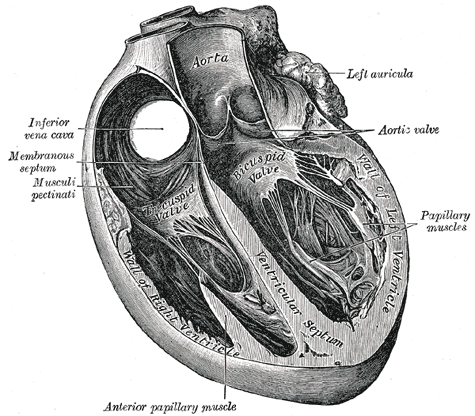
\includegraphics[width=0.7\textwidth]{figures/sample/Gray498.png} 
\caption[Four-chamber illustration of the human heart.]{Four-chamber illustration of the human heart.  Clockwise from upper-left: right atrium, left atrium, left ventricle, right ventricle.}
\label{fig:fourchamber}\end{figure}

The use of acoustic waves for medical diagnosis, inspired by naval sonar, was initially developed in the 1940s \cite{gagliardi_ultrasonography_1996}.  By 1954, the first clinically useful cardiac ultrasound -- examining motion of the mitral valve in stenosis -- was reported \cite{edler_ultrasonic_1957}.  These early scans were one-dimensional images (`A-mode'), sometimes repeated to generate a time axis (`M-mode').   The sector-scanning probe was developed in the 1970s \cite{bom_ultrasonic_1971,griffith_sector_1974}, leading to the `B-mode' that a modern cardiologist would recognise as an echocardiogram.

\chapter{Introduction}
\label{ch:intro}

%\section{Background}
%\label{s:background}

The notion of describing amorphous materials as random networks dates back to \zach, who in 1932 sketched a simple diagram of a \td{} glass \cite{Zachariasen1932}.
This configuration, reproduced in figure \ref{fig:zach_orig}, showed a collection of percolating rings with an absence of long\--range structural ordering.
At the time, \zach's image was intended only as schematic to illustrate the analogous effects in \thd{} glasses.
However, some eighty years later, modern synthesis techniques have yielded a range of \td{} materials including amorphous carbon, silica and germania, which can be considered realisations of \zach's glass \cite{Kotakoski2011,Robertson2012,Huang2012,Lichtenstein2012a,Shaikhutdinov2013,Lewandowski2018,Lewandowski2019}.
These advances may yet represent a watershed moment in chemistry, facilitating the development of a wide range of technologically useful materials with applications including catalysis and gas separation \cite{Trogadas2014,Sun2015a,Buchner2017}.

It is clear that understanding the structure of amorphous materials is key to this aim.
However, due to the relative recentness of these experimental discoveries, much of the existing theory arises from studies of systems on greater length scales.
Specifically, in the second half of the 20\th{} century, much work was carried out on the formation of polycrystals in metals and alloys.
By annealing the metal and slicing through the sample, the grains in the polycrystal could be directly imaged; revealing a system of tessellating polygons not dissimilar to an atomic material \cite{Beck1954,Dunn1957}.

Over time it became apparent that the structure of these networks is constrained on a number of different levels.
Firstly the mean ring size (\ie{} the average number of sides in a polygon) tends to the constant value of six.
This is readily explainable via graph theoretic arguments, resulting from Euler's formula when each vertex forms part of three edges - as is the case for trivalent atoms or the meeting of three grain boundaries.
This is consistent with chemical intuition: a pristine graphene sheet is a hexagonal net and although a Stone\--Wales defect introduces pentagons and heptagons, they occur in pairs to preserve the overall mean ring size \cite{Stone1986}.

The next level of information is then the explicit distribution of polygon sizes, also known as the ring statistics.
With the constraint of a fixed mean, the ring statistics were shown to be relatively well defined, following a lognormal or maximum entropy distribution \cite{Shackelford1981,Lemaitre1993,Lichtenstein2012}.
However, the ring statistics alone are not sufficient to fully describe the network topology. 
This is because the same set of rings can be arranged in a large number of different ways.
Consider again \zach's original configuration. 
Removing one square achieves a mean ring size of six and allows the constituent rings to be arranged as a periodic tiling.
Figures \ref{fig:zach_high}\--\ref{fig:zach_low} show three such example tilings.


\begin{figure}[h]
     \centering
     
     \begin{subfigure}[b]{0.25\textwidth}
         \centering
         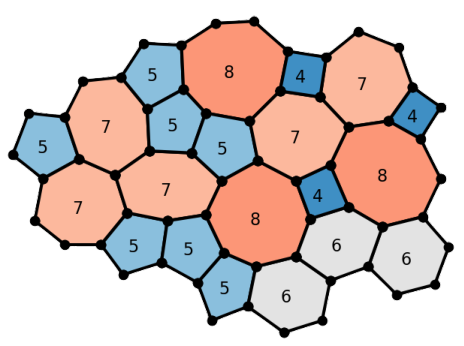
\includegraphics[width=\textwidth]{./figures/introduction/zach_orig.pdf}
         \caption{}
         \label{fig:zach_orig}
     \end{subfigure}
     \hspace{1cm}
     \begin{subfigure}[b]{0.25\textwidth}
         \centering
         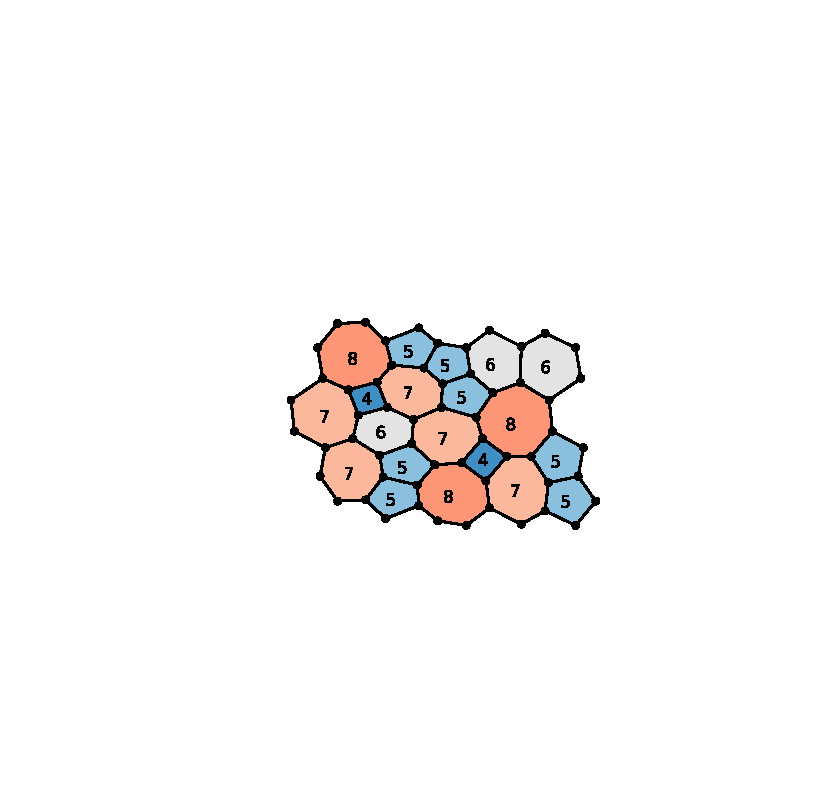
\includegraphics[width=\textwidth]{./figures/introduction/zach_high.pdf}
         \caption{}
         \label{fig:zach_high}
     \end{subfigure}
     
     \begin{subfigure}[b]{0.25\textwidth}
         \centering
         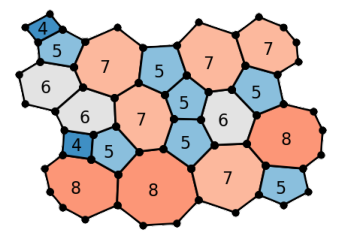
\includegraphics[width=\textwidth]{./figures/introduction/zach_mid.pdf}
         \caption{}
     \end{subfigure}
     \hspace{1cm}
     \begin{subfigure}[b]{0.25\textwidth}
         \centering
         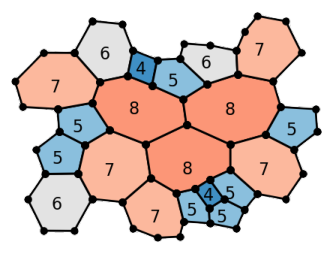
\includegraphics[width=\textwidth]{./figures/introduction/zach_low.pdf}
         \caption{}
         \label{fig:zach_low}
     \end{subfigure}
     
     \caption{Panel (a) shows \zach's glass and panels (b)\--(d) three different periodic arrangements based on the glass (with one square removed to satisfy Euler's formula). Moving from panel (b)\--(d) there is increased clustering of similar sized rings. The size of the rings are highlighted numerically and by colour.}
     \label{fig:zach}
\end{figure}

Whilst they may initially look similar, on closer inspection the three configurations display fundamentally different properties.
In figure \ref{fig:zach_high} similar sized rings are dispersed throughout the arrangement whilst in \ref{fig:zach_low} they are tightly clustered together.
Furthermore, given the large number of configurations which may be theoretically possible for any set of ring statistics, only a subset of these are physically realisable.
Empirically, these are found to be those in which large rings tend to be surrounded by smaller rings \ie{} similar to \ref{fig:zach_high}.
Once again, chemical intuition would support this in the context of atomic materials, as strain is minimised by maintaining bond lengths and angles as close to their equilibrium values as possible.

This effect was first noticed in polycrystals and quantified through the \aw{} law \cite{Aboav1970,Weaire1974}.
This law posits that the mean ring size about any given ring can be related to the central ring size by a single fitting parameter.
Hence the value of this parameter in some way describes the increased tendency of the small rings to be adjacent to large rings.
The \aw{} parameter therefore provides information on the first\--order ring\--ring correlations, completing the topological description of the network material.

The novelty and potential usefulness of \td{} materials makes them a  clear candidate for computational study, in order to complement and supplement experimental endeavours. 
Taking the example of thin silica films, there have already been multiple computational investigations including both \abinitio{} methods and molecular dynamics studies using classical force fields at varying levels of theory \cite{Bjorkman2013,Malashevich2016,Wilson2013,Wilson2018,Zhang2018a,Bamer2019,Roy2019,Richter2019}.
In order to perform these simulations, it is necessary to have a starting atomistic configuration.
This can be achieved in multiple ways. 
The most straightforward is to take one of the existing experimental images. 
These are however limited in size and number and can contain defects or areas which cannot be fully imaged.
In addition, some related experimental systems have proved significantly more challenging to synthesise, such as bilayers of germania, restricting the experimentally available data  \cite{Lewandowski2018,Lewandowski2019}.
As a result, computational techniques are often preferable, but generating configurations will the required topological properties (\ie{} correct ring statistics \textit{and} \aw{} parameter) has proved surprisingly difficult \cite{Roy2018,Kumar2014}.

Therefore, the first part of this thesis will focus on developing methods to generate configurations of \td{} networks in which the topological parameters can be tuned in a controllable manner.
These configurations can then be used as a seed for further computational studies, removing some of the reliance on experimental configurations and opening the door for high\--throughput calculations which can be speculative and potentially predictive.

However, the scope of this work extends beyond materials modelling.
As previously mentioned, much of the original work in this field focussed on polycrystals of metal oxides, with some links to foams and Voronoi polygons \cite{Aboav1980,Boots1984}.
It is now clear that these chemical networks fit into a much wider class of \td{} physical networks that are ubiquitous in the natural world, emerging across physical disciplines and length scales.
Traditional examples range from the atomic level of ultra\--thin materials, through colloids, foams, epithelial cells and all the way to geological rock formations \cite{Earnshaw1994,Allain1995,Moncho-Jorda2000,Durand2011,Tong2017,Goehring2014}.
There are however countless more occurrences, with drying blood, stratocumulus clouds, crocodile scales and geopolitical borders all being the subject of studies \cite{Brutin2011,Glassmeier2017,Milinkovitch2019,LeCaer1993}.

Intriguingly, although these systems are incredibly physically diverse, they have strikingly similar structures \cite{Schliecker1999}. 
This is because they can all be mapped onto the same generic system, which can be equivalently described as a collection of tessellating polygons or percolating rings, and hence they are governed by the same fundamental laws. 
Understanding the behaviours of \td{} networks is therefore key to a wide range of problems in frontier research, not only the directed synthesis of nano\--materials but also for example the control of mitotic division \cite{Gibson2011,Ladan2019}; as well as to curiosities such as explaining the arrangement of the stones in Giant's Causeway or cracking in famous artworks \cite{Weaire1984,Flores2017}.

Coupled with these observations, the continuing expansion and maturity of network science as a field has led to significant advances in the description and characterisation of complex networks.
This has largely been driven by interest in networks in the more abstract sense of the internet, social media and neural networks \cite{Strogatz2001,Boccaletti2006,Barabasi2012}.
To date, the application of these principles in the physical sciences has mostly been confined to topics such as biological signalling pathways.
However, network science is also highly relevant to the study of atomic systems, where the notions of collections of bonded atoms map straightforwardly onto the definition of complex networks as a set of linked nodes.

The second part of this thesis will therefore show how robust metrics from network science can be applied to physical \td{} networks to better quantify their structure and replace the need for empirical measures such as the \aw{} law.
As part of this process, more generic methods will be developed to construct \td{} networks across a range of potential models, coordination environments and topologies.
This will allow a systematic study into the factors which influence the underlying network properties in \td{} systems.
More broadly, this will have the effect of tying physical \td{} networks into the wider field of network science, showing them to be a unique and interesting addition to the area.

The later parts of this thesis will apply the developed concepts and techniques to a series of related and novel problems across chemistry.
To give a broad overview, this will begin with an investigation into the network analysis of quasi\--two\--dimensional hard sphere systems, which is of direct relevance to on\--going experimental studies of colloidal monolayers \cite{Thorneywork2017}.
In such systems, the ring structure emerges through construction of a Voronoi diagram, which partitions the sample space into polygonal regions associated with each particle.
Whilst the properties of Voronoi diagrams are well understood for two\-- and three\--dimensional systems, the intermediate dimensionality of colloidal monolayers leads to novel challenges in their characterisation.

Following this, attention will be turned to another system of relatively recent interest, that of ``procrystalline'' lattices \cite{Overy2016}.
These procrystals can also be considered to have intermediary behaviour, in that they have atoms located on a regular, ordered lattice and yet have disordered ring structure - hence lying between the crystalline and amorphous states.
This partial ordering raises the possibility of procrystals displaying fundamentally different behaviour, in terms of their network properties, to either crystalline or amorphous materials.

Finally, a new tool from topological data analysis, termed persistent homology, will be applied to \td{} amorphous materials.
The aim of persistent homology is to find the fundamental topological features in generic point sets, and so holds the potential to identify and characterise the ring structure in atomic networks \cite{Wasserman2018}.
Although the method is in its relative infancy, the effectiveness of persistent homology in quantifying disorder in the case of \td{} materials can be examined ahead of time through the use of computational models.

These interrelated examples raise two important questions central to this work, namely why is the focus on \td{} systems, and why on computational modelling?
To answer the first of these questions, one may argue it is precisely because there exist experimental realisations of quasi\--two\--dimensional systems, which have a range of technologically useful applications \cite{Butler2013,Bhimanapati2015,Tan2017}.
Alternatively, it may be said that a \td{} system is in some way a simplified version of a \thd{} assembly, and so they provide a tractable way of studying the behaviours of higher dimensionality systems.
Whilst both these statements have merit, neither is entirely satisfactory, as the former neglects to explain why such experiments are successful and latter is not universally true \cite{ChaikinPaulM1995}.
Two\--dimensional systems can display their own unique constraints, which in fact often leads to the desirable properties of nanomaterials.

What study in two dimensions provides, is the opportunity to visualise, analyse and understand systems which are inherently more tangible.
Raw data is available experimentally in real\--space, without the need for transformation, as required for example with structure factors or diffraction patterns.
From this data, metrics such as the ring structure are well defined and readily extractable.
This in turn allows the development of simulation and analysis methods which are able to accurately model and characterise the system, leading to a more complete understanding.
Ideally, the insight gained can be applied to higher dimensions, or used to aid the synthesis of materials with desired properties.

In response to the second question, the power of computational modelling as complement to experiment arises from the ability to reproduce experimental results, but also explore experimentally inaccessible systems.
As previously mentioned, experimental microscopy data from frontier research is difficult to produce and may be incomplete or relatively small in extent.
Computational models can help to bridge any gaps and provide information as to the frequency or stability of the observed sample.
Moreover, computation has direct access to a greater number of observables than experiment, which can help provide explanation for a given phenomenon.
Finally, and perhaps most importantly, simulation allows a holistic study of materials by continuously varying parameters to generate structures which may or may not map onto those from experiment.
This enables properties to systematically explored, in principle leading to the holy grail of computational modelling, that of predictive capability.

This thesis will incorporate many of the above aspects to investigate the phenomenon of structural disorder in \td{} network\--forming materials.
Computational models and methods will be developed to simulate a wide range of \td{} systems.
This will be achieved almost exclusively through the use of stochastic \mc{} algorithms.
These tools will be designed with flexibility in mind, aiming to generate configurations in which the ring topologies can be precisely controlled.
In most cases, whilst the underlying models will remain physically motivated, the specificities of the system will be abstracted into a more generic network problem.
This will allow comparisons to be made between initially seemingly disparate materials and enable development of a generalised network theory for physical \td{} systems.

Nevertheless, the motivation for this work is still ultimately grounded in the characterisation and development of real materials.
Contact will therefore be made to experimental results and the applicability and relevance to experimental investigations will be detailed throughout.
In particular, this thesis will aim to improve the modelling of amorphous bilayers, evaluate analysis methods for thin\--films and colloidal packings, and direct the synthesis of procrystalline materials.  

%\section{Thesis Structure}
%
%The structure of this thesis is as follows:
%\davidnote{Todo: thesis structure}
%\davidnote{Just basically a repeat of abstracts?}
%\davidnote{Actually can this section just go?}
%
%\begin{itemize}
%	\item \textbf{Chapter 2}: the theory underpinning complex networks is discussed, covering the representation of atomic systems as networks and the relationship of the dual network to ring structure.
%The laws which govern the topological properties of physical networks are also introduced, namely Euler's law, \lm's law and the \aw{} law.
%
%	\item \textbf{Chapter 3}: the theoretical basis of \mc{} methods and their application to generating realisations of \td{} networks is reviewed.
%There is a broad discussion of Metropolis \mc{} methods, before specific methods are covered in detail; namely the bond switching algorithm and hard particle \mc{} in conjunction with the Voronoi construction.
%This discussion lays the groundwork for the extension of these methods and development of additional \mc{} algorithms in subsequent chapters.
%	
%	\item \textbf{Chapter 4}: a computationally tractable \mc{} method using triangle rafts is developed to generate bilayers of \sioii{} and related materials.
%The method allows defect free networks of any given shape to be grown with both tuneable ring statistics and topologies, controlled by a combination of the choice of the ``allowed'' rings and the effective growth ``temperature''. 
%Configurations are generated with \aw{} parameters commensurate with those obtained from an analysis of experimental configurations, improving significantly on previous methods.
%The ability to efficiently grow configurations allows exploration of the structural basis of \lm’s law, where the commonly observed value of $p_6\approx0.4$ is presented as a balance between entropic and enthalpic factors. 
%The deviations of ring areas from the ideal values are discussed and the relative insensitivity of the ring area to relatively strong distortions is highlighted.
%	
%	\item \textbf{Chapter 5}:
%	
%	\item \textbf{Chapter 6}:
%	
%	\item \textbf{Chapter 7}:
%	
%	\item \textbf{Chapter 8}:
%
%	\item \textbf{Chapter 9}:
%	
%	\item \textbf{Chapter 10}:
%\end{itemize}
	
 

\chapter{Computational Methods}
\label{ch:compmethods}

\begin{chapterabstract}
The theoretical basis of \mc{} methods and their application to generating realisations of \td{} networks is reviewed.
There is a broad discussion of Metropolis \mc{} methods, before specific methods are covered in detail; namely the bond switching algorithm and hard particle \mc{} in conjunction with the Voronoi construction.
Extensions to these methods and additional approaches are outlined in the relevant chapters \davidnote{Link to bond switching/Voronoi/mx2/procrystals later}.
\end{chapterabstract}

\section{General \mc{} Methods}
\label{sec:mc}

\mc{} methods are a class of computational algorithms designed to solve complex problems stochastically.
These normally fall into the broad categories of calculating integrals, sampling probability distributions and finding global minima of very high dimensional functions \-- tasks which are often incredibly hard to compute deterministically.
Since their initial development in the mid\--20\th{} century, such methods have become an invaluable tool for solving problems in the physical sciences.
\mc{} methods are used in this context for calculating thermodynamic averages of properties in equilibrium systems; finding the minima in potential energy surfaces of small molecules, glasses, crystals and biomolecules; as well as non\--equilibrium simulations such as growth of crystals and thin\--films \cite{Landau2014,Wales1999,Levi1997,Ratsch2003,Kob1999,Jensen1999}.
In this thesis these \mc{} methods  will be used in a variety of contexts chapter xxx \davidnote{fill this in}.
Therefore, the general theory is presented here with specific details of two established methods: bond switching and hard particle \mc{} given in the following section.

\subsection{Statistical Mechanics}

The total energy of a system with a fixed number of particles, $\mathcal{N}$, is given by the Hamiltonian,
\begin{equation}
	\ham = \ken+\pen \,,
\end{equation}
where $\ken$ is the kinetic energy as a function of all particle momenta and $\pen$ is the potential energy as a function of all particle positions \cite{Frenkel2002}.
The positions and momenta comprise the phase space of the system.
At fixed volume, $\mathcal{V}$, and temperature, $T$, all the the essential thermodynamic information is then provided through the classical canonical partition function:
\begin{equation}
	Q = \frac{1}{h^{D\mathcal{N}}\mathcal{N}!}\int \dd\mathbf{p}\,\dd\mathbf{r}\,\exp{\left[-\ham/ \kb T\right]}\,,
\end{equation}
where $D$ is the number of spatial dimensions.
This can be factorised into kinetic and potential components as
\begin{equation}
	Q = \frac{1}{h^{D\mathcal{N}}\mathcal{N}!}\int \dd\mathbf{p}\,\exp{\left[-\ken/\kb T\right]} \int \dd\mathbf{r}\,\exp{\left[-\pen/\kb T\right]} \,,
\end{equation}
where
\begin{equation}
	Z = \int \dd\mathbf{r}\,\exp{\left[-\pen/\kb T\right]}
\end{equation}
is the configurational integral \cite{Allen2017}. 
As will be shown, in \mc{} simulations it is the energetic differences between configurations that are required, and so at constant temperature the kinetic component can be neglected and it is only the configurational integral that is of importance.
In this case the probability density of the system being in the configuration $\mathbf{r}$ is given by the Boltzmann distribution:
\begin{equation}
	\label{eq:boltzmann}
	P\left(\mathbf{r}\right) = \frac{\exp{\left[-\pen/\kb T\right]}}{Z}\,.
\end{equation}
This allows the expectation value of an observable of the system, $\obs$, to be determined from:
\begin{equation}
	\label{eq:expectationobs}
	%\langle A \rangle = \frac{1}{Z}\int \dd\mathbf{r}\,\obs\exp{\left[-\pen/\kb T\right]} \,.
		\langle A \rangle = \int \dd\mathbf{r}\,\obs P\left(\mathbf{r}\right) \,.
\end{equation} 
The expectation value is then the ratio of two $\mathcal{N}D$ dimensional integrals.
The next section shows how these can be evaluated by \mc{} sampling.

\subsection{Importance Sampling}

An integral of form \eqref{eq:expectationobs} can be evaluated numerically by a number of methods.
As an illustration, consider the simple example of a \td{} potential energy surface in figure \ref{fig:montecarloint}.
To calculate the expectation value of the potential energy one must evaluate the integral
\begin{equation}
	\langle \mathcal{U} \rangle = \int_{0}^{L_y}\int_{0}^{L_x} \dd x \dd y\, \mathcal{U}\left(x,y\right)\mathcal{P}\left(x,y\right)\,.
\end{equation}
One way to achieve this would be to use standard numerical methods such as the trapezium rule or Simpson's rule to calculate the potential energy over a regular grid of points, as in figure \ref{fig:montecarloint1}, weighting each according to the Boltzmann distribution.

An alternative would be to take a stochastic approach.
In the simplest implementation, a series of $S$ random sampling points, $\left(x_i,y_i\right)$, can be generated uniformly in the intervals $\left[0,L_x\right]$ and $\left[0,L_y\right]$, as in figure \ref{fig:montecarloint2}.
Weighting these according to the Boltzmann distribution and averaging gives an estimation to the integral:
\begin{equation}
	\langle \mathcal{U} \rangle = \frac{L_xL_y}{S}\sum_{i=1}^{S} \mathcal{U}\left(x_i,y_i\right)\mathcal{P}\left(x_i,y_i\right)\,,
\end{equation}
which converges to the exact value as $S\rightarrow\infty$.

However, both quadrature and \mc{} uniform sampling suffer from the same inefficiency.
As can be seen in both schemes, many of the sampling points fall in regions of phase space where the potential energy is high and hence the weighting probability distribution is very small at reasonable temperatures.
In effect, significant effort is spent calculating regions where the contribution to the total integral is negligible.
A better approach is therefore to generate a series of $S$ random sampling points, $\left(x_i,y_i\right)$, according to the distribution $\mathcal{P}\left(x,y\right)$, as in figure \ref{fig:montecarloint2}.
The expectation value of the observable can then be calculated using a simple average:
\begin{equation}
	\langle \mathcal{U} \rangle = \frac{1}{S}\sum_{i=1}^{S} \mathcal{U}\left(x_i,y_i\right)\,.
\end{equation}
This is known as importance sampling and is vastly more efficient when dealing with an aggressive probability distribution like the Boltzmann, where only a small proportion of the phase space is accessible.

\begin{figure}[bt]
     \centering
     
     \begin{subfigure}[b]{0.45\textwidth}
         \centering
         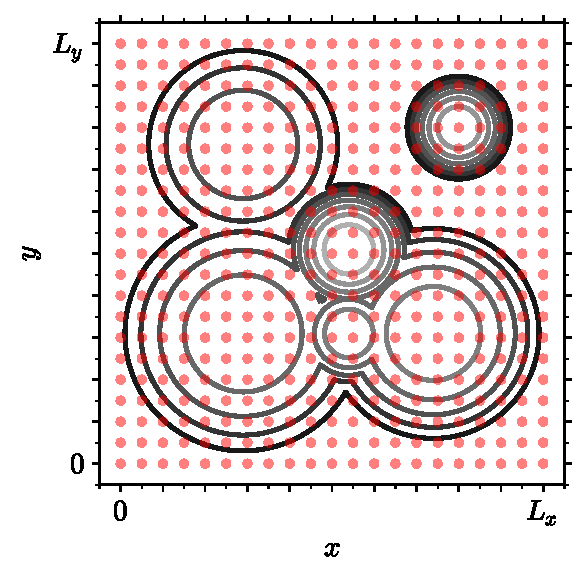
\includegraphics[width=\textwidth]{./figures/methods/mc_2d_quad.pdf}
         \caption{Quadrature.}
         \label{fig:montecarloint1}
     \end{subfigure}
     \hfill
     \begin{subfigure}[b]{0.45\textwidth}
         \centering
         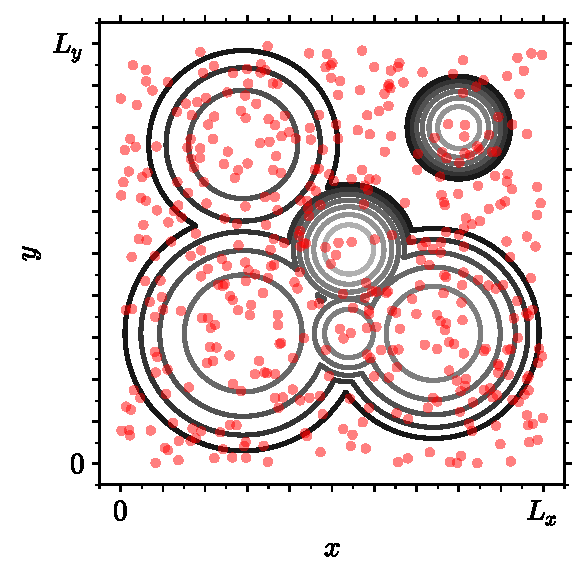
\includegraphics[width=\textwidth]{./figures/methods/mc_2d_rand.pdf}
         \caption{Uniform Sampling.}
         \label{fig:montecarloint2}
     \end{subfigure}
     \hfill
     
     \begin{subfigure}[b]{0.45\textwidth}
         \centering
         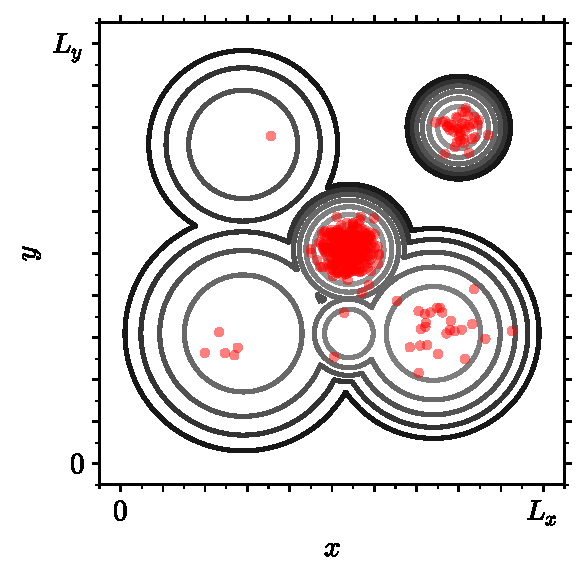
\includegraphics[width=\textwidth]{./figures/methods/mc_2d_imp.pdf}
         \caption{Importance Sampling.}
         \label{fig:montecarloint3}
     \end{subfigure}
     \hfill
     \begin{subfigure}[b]{0.45\textwidth}
         \centering
         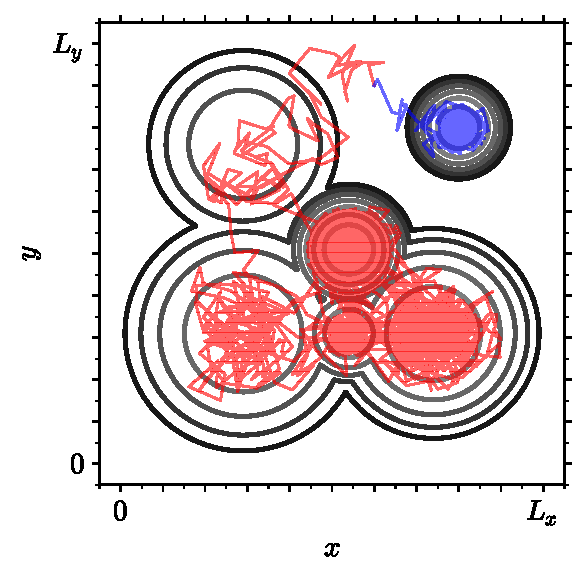
\includegraphics[width=\textwidth]{./figures/methods/mc_2d_mcmc.pdf}
         \caption{Markov Chain \mc}
         \label{fig:montecarloint4}
     \end{subfigure}
     \hfill
    
     \caption{Demonstration of different sampling methods with an example \td{} potential energy surface (contour lines). Panels(a)\--(c) display the same number of (red) sampling points. Panel (a) shows conventional quadrature where the surface is divided into a regular grid of sampling points which are then weighted by the Boltzmann distribution. Panel (b) shows \mc{} sampling with a uniform distribution of points which again must be Boltzmann\--weighted. Panel (c) shows \mc{} importance sampling with points now selected according to the Boltzmann distribution. Panel (d) shows Markov chain \mc{} with two random walks through phase space (red and blue lines) starting from different random seeds.}
     \label{fig:montecarloint}
\end{figure}

Whilst this scheme is ideal theoretically, it is impracticable for physical systems.
This is because for any problem of real interest one lives in a ``black box'' where the functional form of the potential energy surface in its hundreds if not thousands of dimensions is unknown.
In this case often the only way of learning about the form is by on\--the\--fly exploration of the surface \cite{Brooks2011}.
This can be achieved by talking a random walk through configurational space using Markov chain \mc.

\subsection{Markov Chain Monte Carlo}

Markov chain Monte Carlo provides a framework to perform importance sampling on a potential energy surface.
A system of interest can exist in a (very large) number of configurational states, $\left\{\mathbf{r}_0,\mathbf{r}_1,\dots,\mathbf{r}_M\right\}$.
A Markov chain can then be constructed from this set, whereby a sequence of states is generated stochastically across a series of steps, $s=0,1,\dots,S$.
In this process, the probability of moving between states at each step is given by the transition matrix, $\bm{\pi}$, where each element, $\pi_{ij}$, gives the probability of moving from the state $\mathbf{r}_i$ to another state $\mathbf{r}_j$.  
This leads to the two relationships:
\begin{align}
	0\leq \pi_{ij} &\leq 1\,, \\
	\sum_{j} \pi_{ij} &= 1\,, \label{eq:tmrowsum}
\end{align}
the first being a statement of the probabilistic nature of the elements whilst the second ensures all transfer remains within the state space \cite{Frenkel2002,Allen2017,Brooks2011}.

The probability that the system is in each state at a given step, $s$, can be represented by the row vector $\mathbf{P}_s$.
This probability distribution evolves with each step as $\mathbf{P}_{s+1}=\mathbf{P}_{s}\bm{\pi}$, so that starting from any initial distribution, $\mathbf{P}_0$, it follows that $\mathbf{P}_S=\mathbf{P}_0\bm{\pi}^S$. 
The question is then as to the behaviour as $S\rightarrow \infty$.
Provided certain criteria are met, the distribution will tend to a stationary distribution, $\mathbf{P}$, which satisfies the eigenvalue equation 
\begin{equation}
	\mathbf{P} = \mathbf{P}\bm{\pi}\,, \label{eq:mcmceig}
\end{equation}
regardless of the initial distribution (although the speed of the convergence does depend on $\mathbf{P}_0$).
This will occur only if the system is \textit{ergodic}, meaning that every state is connected to every other by some finite path.

In a discrete analogue to equation \eqref{eq:expectationobs}, the expectation value of an observable, $A$, can be calculated from the ensemble average:
\begin{equation}
	\langle A \rangle = \sum_{i=1}^{M} A\left(\mathbf{r}_i\right)\mathcal{P}\left(\mathbf{r}_i\right)\,,
\end{equation}
where $\mathcal{P}\left(\mathbf{r}_i\right)$ are the elements of $\mathbf{P}$.
However, as previously mentioned the number of discrete states is usually exceedingly large and so calculating the average over all states is not possible.
The solution is to take a random walk across through configurational space, sampling explicit states to form the chain $X_0,X_1,\dots,X_S$; where each move is chosen randomly according to the transition matrix $\bm{\pi}$.
In this case the expectation of the same observable can be calculated from the average over the sampled states:
\begin{equation}
	\langle A \rangle = \frac{1}{S}\sum_{i=1}^{S} A\left(X_i\right)\,,
\end{equation}
where the true value is approached as $S\rightarrow \infty$.

In this section the problem of sampling phase space efficiently has been reformulated, but as yet not solved. 
This is because the form of the transition matrix is still unknown.
Instead only the ideal form of the limiting probability distribution, $\mathbf{P}$, is available \-- where the elements follow the Boltzmann probabilities in equation \eqref{eq:boltzmann}.
A practical solution to this problem is provided by the Metropolis algorithm.

\subsection{Metropolis Algorithm}
\label{ssec:metropolis}

The Metropolis algorithm gives a prescription of how to construct a transition matrix, $\bm{\pi}$, with the requisite properties that samples the Boltzmann distribution \cite{Metropolis1953}.
Firstly, combining equations \eqref{eq:tmrowsum} and \eqref{eq:mcmceig} gives a condition on the transition matrix known as global balance:
\begin{equation}
	\sum_j \mathcal{P}\left(\mathbf{r}_i\right)\pi_{ij} = \sum_j \mathcal{P}\left(\mathbf{r}_j\right)\pi_{ji}\,.
\end{equation} 
Whilst it is possible to construct transition matrices which satisfy only global balance \cite{Manousiouthakis1999,Suwa2010,Michel2014}, it is practically simpler to satisfy global balance by applying the stronger condition of detailed balance:
\begin{equation}
	\mathcal{P}\left(\mathbf{r}_i\right)\pi_{ij} = \mathcal{P}\left(\mathbf{r}_j\right)\pi_{ji}\,.
\end{equation}
In the Metropolis algorithm the off\--diagonal elements of the transition matrix are written as the product of two probabilities: 
\begin{equation}
	\pi_{ij} = \begin{cases} 
		\tau_{ij}P_{ij} \quad & i\neq j \\
		1-\sum\limits_{j\neq i}\tau_{ij}P_{ij} \quad & i=j
	\end{cases}\,,
\end{equation}
where $\tau_{ij}$ is the trial probability of moving from state $\mathbf{r}_i$ to $\mathbf{r}_j$ and $P_{ij}$ is the probability of accepting the trial move.
To conform to detailed balance, the trial probabilities must be chosen to satisfy $\tau_{ij}=\tau_{ji}$.
Then, in the crux of the algorithm, the acceptance probabilities are given by
\begin{align}
	 P_{ij}&=\begin{cases}
	 	1 \quad &\mathcal{P}\left(\mathbf{r}_j\right)\geq \mathcal{P}\left(\mathbf{r}_i\right) \\
	 	\frac{\mathcal{P}\left(\mathbf{r}_j\right)}{\mathcal{P}\left(\mathbf{r}_i\right)} \quad & \mathcal{P}\left(\mathbf{r}_j\right)< \mathcal{P}\left(\mathbf{r}_i\right)
	 \end{cases}
	 =\begin{cases}
	 	1 \quad &\mathcal{U}\left(\mathbf{r}_j\right)\leq \mathcal{U}\left(\mathbf{r}_i\right) \\
	 	\frac{\exp\left[-\mathcal{U}\left(\mathbf{r}_j\right)/\kb T\right]}{\exp\left[-\mathcal{U}\left(\mathbf{r}_i\right)/\kb T\right]} \quad & \mathcal{U}\left(\mathbf{r}_j\right)>\mathcal{U}\left(\mathbf{r}_i\right)
	 \end{cases}\,,
\end{align}
which can be expressed more succinctly as
\begin{equation}
	\label{eq:metropolis}
	 P_{ij}=\text{min}\big[1,\exp\left[-\Delta \mathcal{U}/\kb T\right]\big]\,,
\end{equation}
where $\Delta \mathcal{U}$ is the difference in potential energy between the final and initial states.
The elegance of the Metropolis algorithm lies in the fact that the acceptance probability depends only on the ratio of the configuration probabilities removing the need for a normalising factor.
This means the relative probabilities can be used (which are computable) instead of the absolute probabilities (which are unknowable).

The final stage is the choice of the matrix of trial probabilities, $\bm{\tau}$. 
This is very flexible and one can be creative in the selection of trial moves, providing that the underlying matrix is symmetric and ergodic.
An effective strategy is to choose moves in which the trial state is relatively close to the current state to trace the paths of high probability in the system.
A summary of the Metropolis algorithm is therefore as follows:
\begin{enumerate}
	\item Initialise the system in a state $X_{s=0}$ and calculate the potential energy $\mathcal{U}\left(X_s\right)$
	\item Generate a trial state $X_t$ (a perturbation of $X_s$) according to $\tau_{st}$
	\item Calculate the potential energy of the trial state $\mathcal{U}\left(X_t\right)$
	\item Determine acceptance or rejection of the trial move according to the Metropolis criterion \eqref{eq:metropolis}
	\item Update the system to the new state: if the trial move is accepted $X_{s+1}=X_{t}$ otherwise $X_{s+1}=X_{s}$
	\item Repeat steps 2\--5
\end{enumerate}
There are a few practical factors related to the scheme above.
In Markov chain \mc{} it was previously mentioned that it takes time for the system to evolve to the stationary distribution.
Therefore it is necessary to have an equilibration period where the chain is generated but not used for sampling of observables.
In addition, whilst selecting trial moves close to the current state increases efficiency, it introduces correlation into the procedure.
A way around this is to not calculate observables based on every step, but rather after a number of statistically significant steps.

As an example of the Metropolis algorithm, consider again the \td{} potential energy surface in figure \ref{fig:montecarloint4}.
Here two simulation paths are displayed in red and blue, starting from the same initial state but with different starting points in the random number generators \ie{} random seeds.
As can be seen the Metropolis algorithm takes a random walk over the configurational space, conducting importance sampling as in \ref{fig:montecarloint3}.
However, in this example highlights a potential problem.
There are two regions of phase space with non\--zero probabilities which are separated by a relatively large energy barrier.
Although they are in principle linked by a path, the barrier may effectively mean they are disconnected on a reasonable simulation time scale, breaking ergodicity.
This manifests as the red walk sampling one region and the blue walk being trapped in the other region.
Using multiple seeds in this way helps to identify if any such behaviour is present.
If it leads to significant differences in the computed averages, more advanced techniques using enhanced sampling may have to be employed \cite{Torrie1977,Earl2005}.

\subsection{Global Optimisation \& Simulated Annealing}
\label{s:simulatedannealing}

So far in this section it has been shown how Monte Carlo methods can be used perform importance sampling of potential energy surfaces.
These methods can also be used to solve the related problem of finding global minima in potential energy surfaces and other more general functions.
Consider the case where there is an objective function, $\obj\left(\mathbf{r}\right)$, which depends on particle positions.
If it is known that there exists a solution where $\obj\left(\mathbf{r}\right)=0$, it may be sufficient to perform a standard random walk of the type in figure \ref{fig:montecarloint4} until a solution is found, using the more general Metropolis criterion:
\begin{equation}
	\label{eq:objmetropolis}
	P_{ij} = \min\big[1,\exp\left[-\Delta\Omega/\kb T\right]\big].
\end{equation}
There is of course a chance that the optimisation will not converge to the global minimum, most likely getting trapped in a local minimum (as for instance the blue path in \ref{fig:montecarloint4}).
One solution to this problem is just to keep restarting the algorithm with different initial conditions until the global minimum is obtained.

Often however the value of the global minimum is not known, as is the case for a potential energy surface, and this rudimentary approach is insufficient.
One must then employ a more sophisticated technique to find the global minimum of a very high dimensional and potentially rough surface.
This in itself is an extensive area of study and there are many approaches such as using genetic algorithms or basin\--hopping \cite{Hartke1993,Niesse1996,Wales1997}.
This thesis will use simulated annealing, which can be considered an extension to Metropolis \mc{} \cite{Kirkpatrick1983}.
In addition simulated annealing is effective for searching surfaces with many similar minima as in glasses \-- the name reflecting its origins in the analogous process in metallurgy to generate defect free metals.

\begin{figure}[tb]
     \centering
    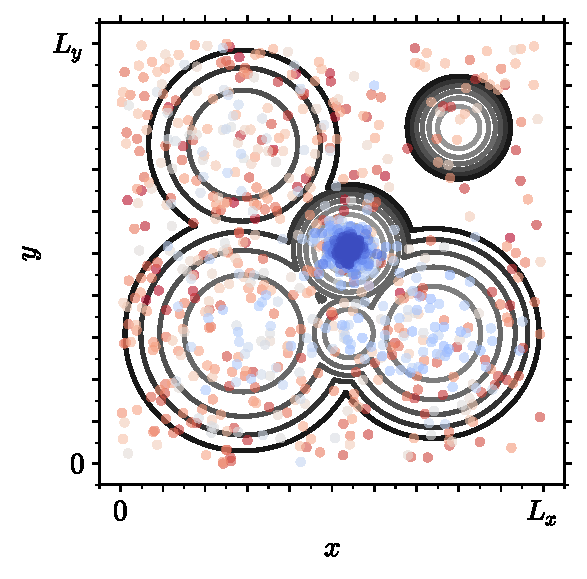
\includegraphics[width=0.45\textwidth]{./figures/methods/mc_2d_sa.pdf}
      \caption{Demonstration of the simulated annealing algorithm on a \td{} potential energy surface, with states coloured by temperature (red$\rightarrow$blue indicating hot$\rightarrow$cold. As the temperature is reduced the state converges on the global minimum.}
      \label{fig:montecarloint5}
\end{figure}

The simulated annealing algorithm proceeds as follows.
The system of interest is first thermalised by performing Metropolis \mc{} at infinite temperature \ie{} accepting every move. 
The system is then gradually cooled to zero temperature, with the Metropolis criterion \eqref{eq:objmetropolis} reducing the proportion of accepted moves.
In theory if the cooling is infinitely slow, the system is maintained in thermal equilibrium and will eventually reach the global minimum \cite{Henderson2003}.
In practice this is not realisable and so a cooling rate must be empirically selected.
Still it is possible for trapping to occur in local minima, especially if the transition between low energy states is very slow.
As before, one can then cycle the simulated annealing, repeatedly heating and cooling the system until the global minimum is found.
The simulated annealing algorithm is demonstrated with the \td{} potential energy surface in figure \ref{fig:montecarloint5}.
As can be seen at high temperature the entire surface is sampled, overcoming all energy barriers, but as cooling takes place the system settles into the low energy regions of the surface, finally terminating in the global minimum.

\section{Bond Switching Monte Carlo}
\label{s:bondswitch}

Bond switching Monte Carlo was originally developed by Wooten, Winer and Weaire to generate high quality configurations of three dimensional silica glass \cite{Wooten1985}.
The basic principle is to amorphise a crystalline lattice with a series of transformations that swap the nearest neighbours of pairs of atoms and optimise the resulting structure to generate a continuous random network which is well\--relaxed.
These continuous random network models replicate experimental observables with high accuracy (including bond length and angle distributions, radial distribution functions, electronic band gaps and Raman spectra) and have since been applied to alternative systems such as three\--dimensional amorphous carbon, binary glasses and biological polymers \cite{Treacy2012,Tu1998,Djordjevic1995,Mousseau2004,Huisman2008,Broedersz2014}.
However, the method can also be readily modified to study \td{} systems, as has been done for amorphous graphene and silica, and which forms the basis for much of the work in this thesis \davidnote{ref to later chapters} \cite{Kumar2014,Jain2018}.
The basic algorithmic details are described in this section, with extensions given in sections \davidnote{again ref later}.

\subsection{Algorithmic Details} 

The \td{} bond switching algorithm essentially follows the prescription of simulated annealing in section \ref{s:simulatedannealing}.
A skeleton algorithm structure is outlined below, followed by specific details \cite{Kumar2012}.
Visualisations are provided for reference in figure \ref{fig:bsmc}.

\begin{enumerate}
	\item Generate initial crystalline hexagonal lattice
	\item Thermalise the lattice with a large number of random moves 
	\item Sample configurations by annealling the system slowly at finite temperature, accepting moves according to the Metropolis criterion \ref{eq:metropolis}
\end{enumerate}
\begin{figure}[bt]
     \centering
     
     \begin{subfigure}[b]{0.24\textwidth}
    \centering
         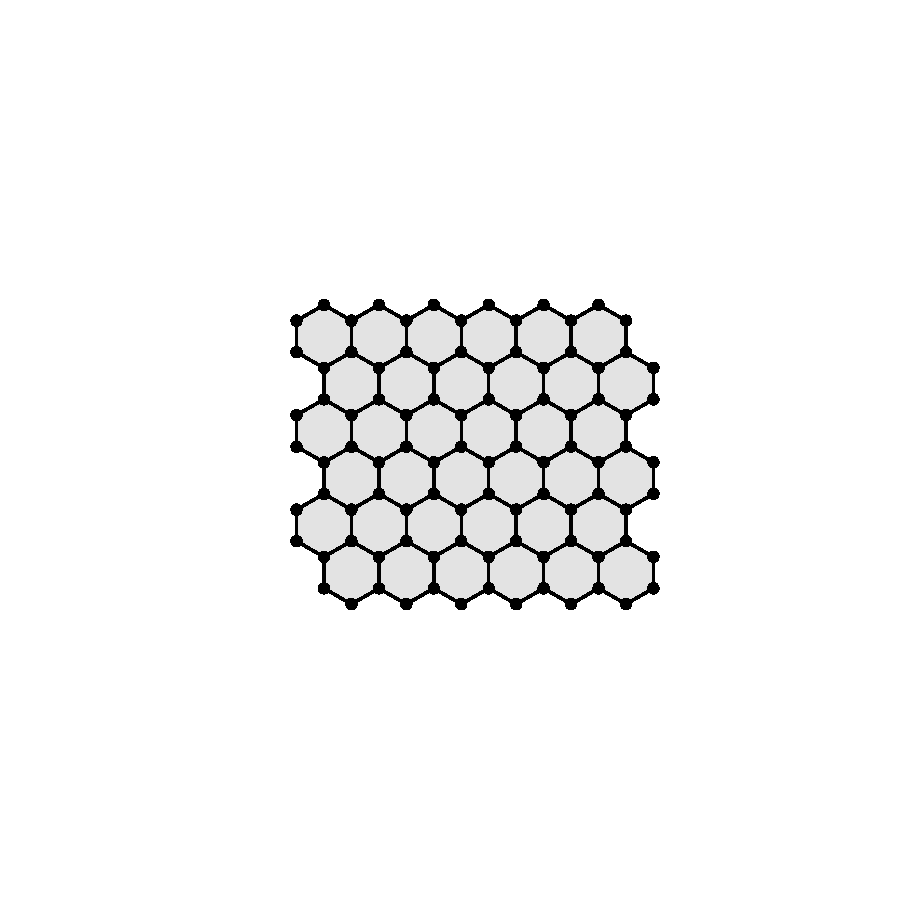
\includegraphics[height=2.8cm]{./figures/methods/bs_0.pdf}
         \caption{}
         \label{fig:bsmc1}
     \end{subfigure}
     \hfill
     \begin{subfigure}[b]{0.24\textwidth}
    \centering
         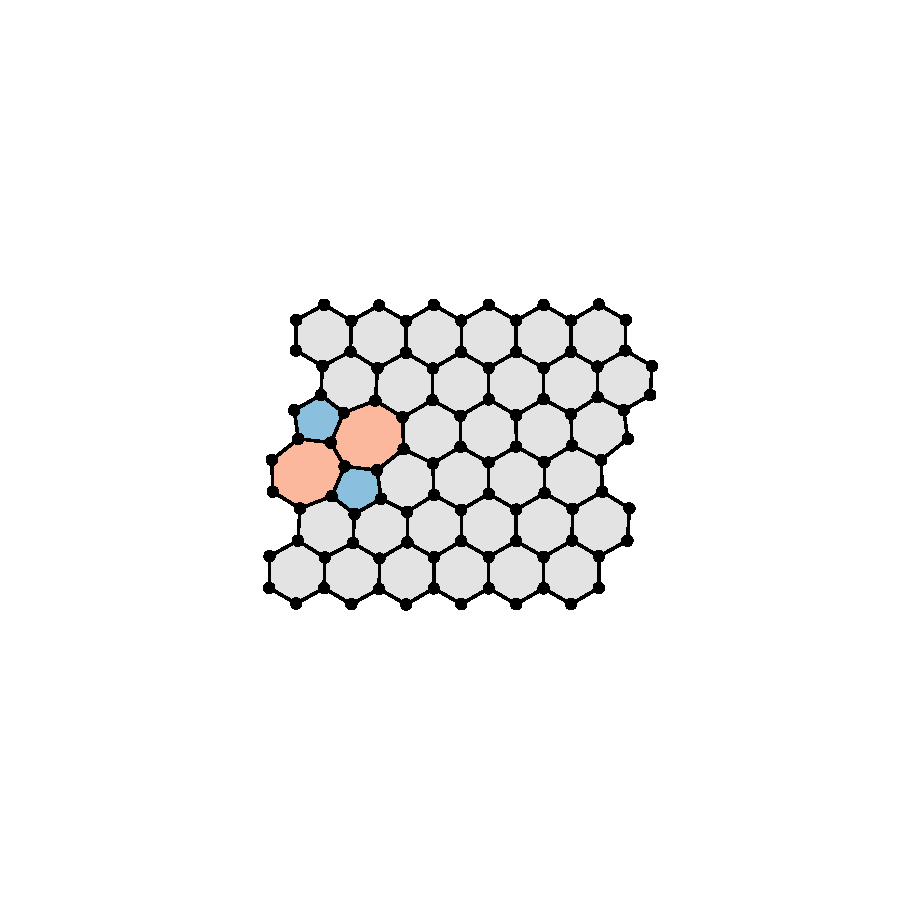
\includegraphics[height=2.8cm]{./figures/methods/bs_1.pdf}
         \caption{}
         \label{fig:bsmc2}
     \end{subfigure}
     \hfill
     \begin{subfigure}[b]{0.24\textwidth}
    \centering
         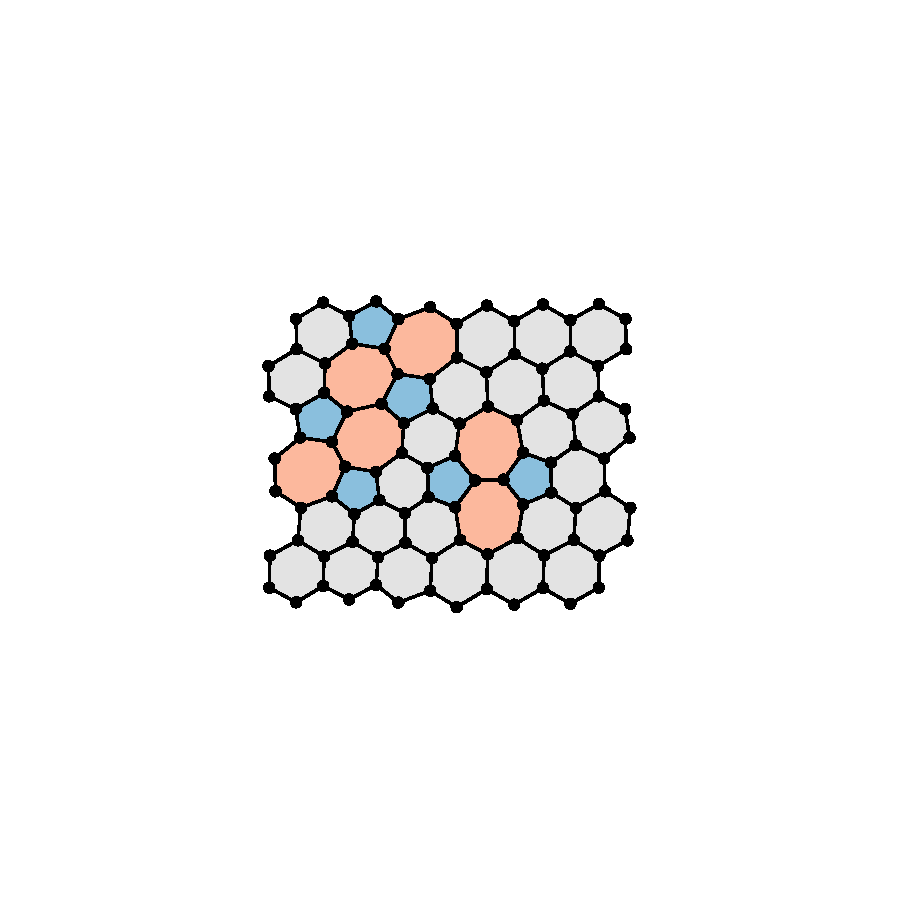
\includegraphics[height=2.8cm]{./figures/methods/bs_3.pdf}
         \caption{}
         \label{fig:bsmc3}
     \end{subfigure}
     \hfill
     \begin{subfigure}[b]{0.24\textwidth}
    \centering
         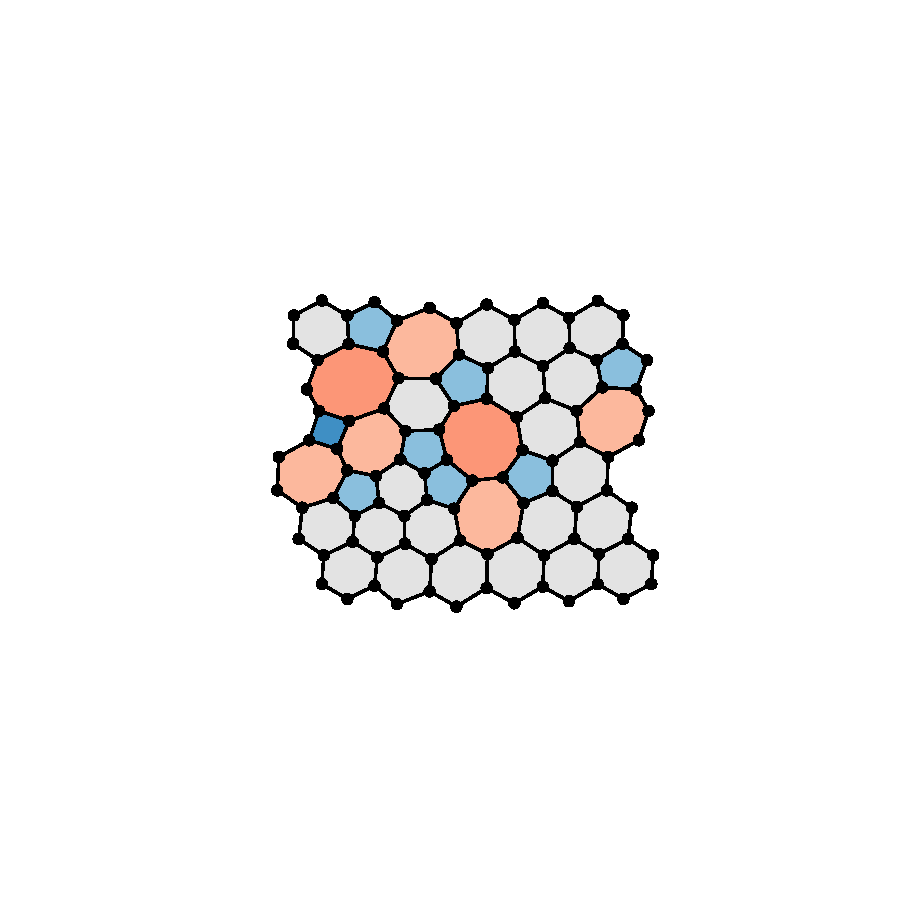
\includegraphics[height=2.8cm]{./figures/methods/bs_5.pdf}
         \caption{}
         \label{fig:bsmc4}
     \end{subfigure}
     
     \begin{subfigure}[b]{0.24\textwidth}
     \centering
         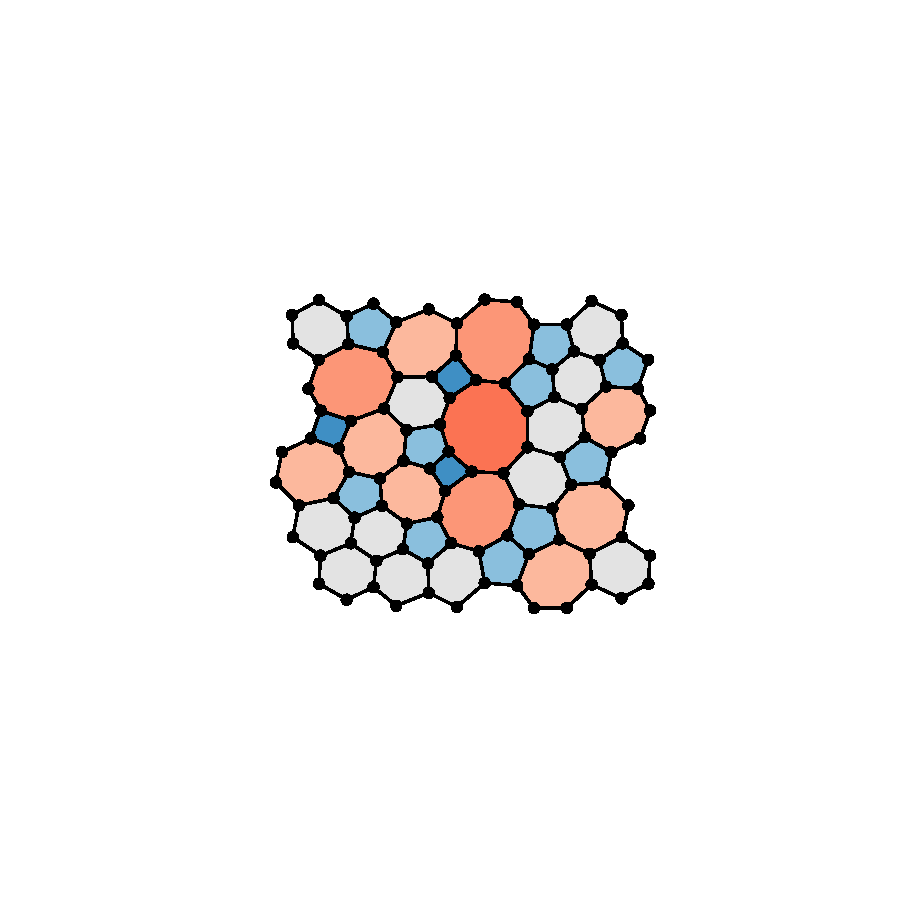
\includegraphics[height=2.8cm]{./figures/methods/bs_10.pdf}
         \caption{}
         \label{fig:bsmc5}
     \end{subfigure}
     \hfill
        \begin{subfigure}[b]{0.24\textwidth}
    \centering
         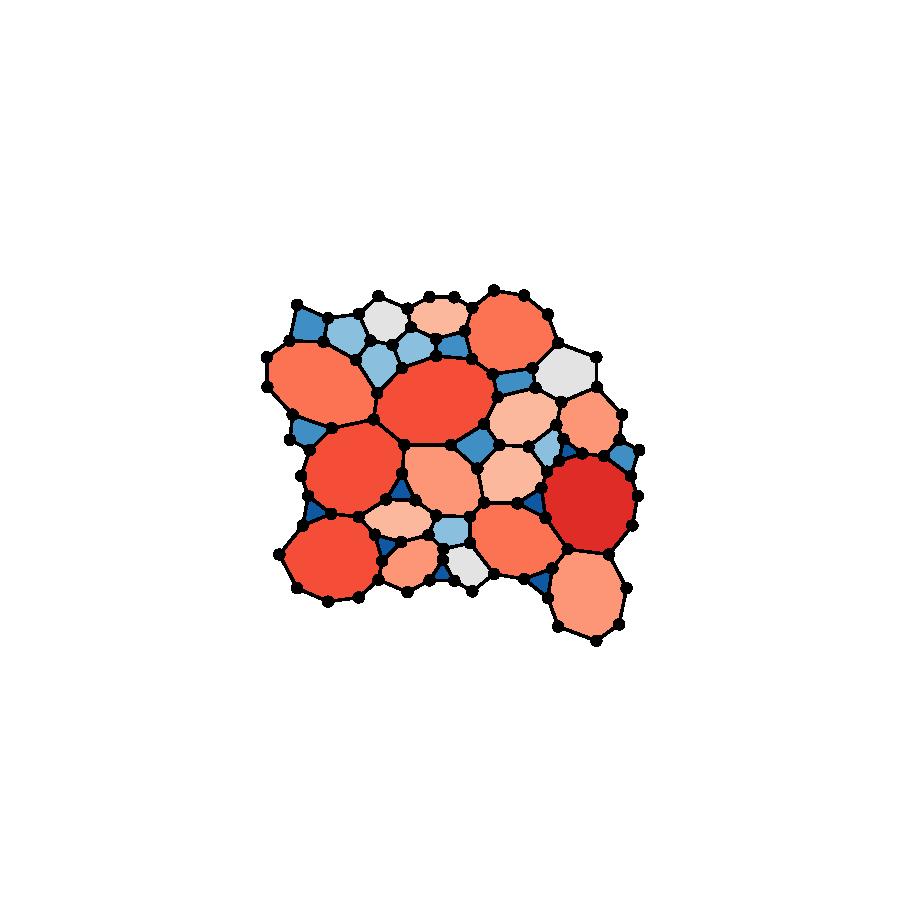
\includegraphics[height=2.8cm]{./figures/methods/bs_1000.pdf}
         \caption{}
         \label{fig:bsmc6}
     \end{subfigure}
     \hfill
           \begin{subfigure}[b]{0.24\textwidth}
    \centering
         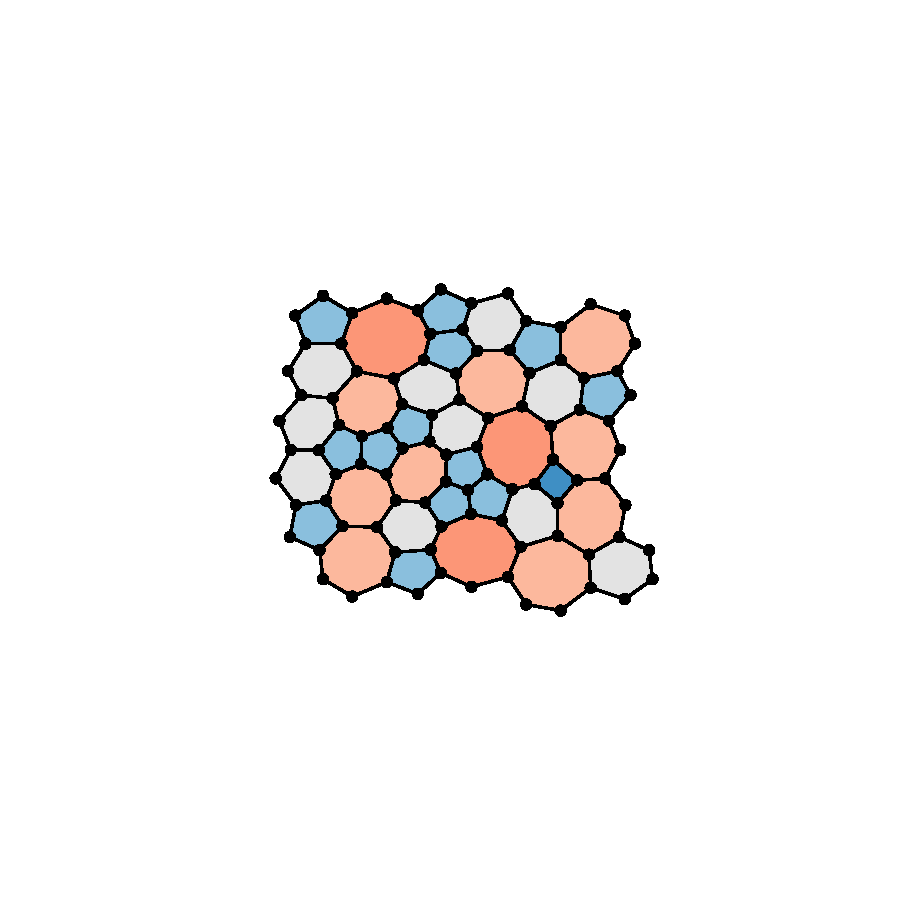
\includegraphics[height=2.8cm]{./figures/methods/bs_t1.pdf}
         \caption{}
         \label{fig:bsmc7}
     \end{subfigure}
     \hfill
           \begin{subfigure}[b]{0.24\textwidth}
    \centering
         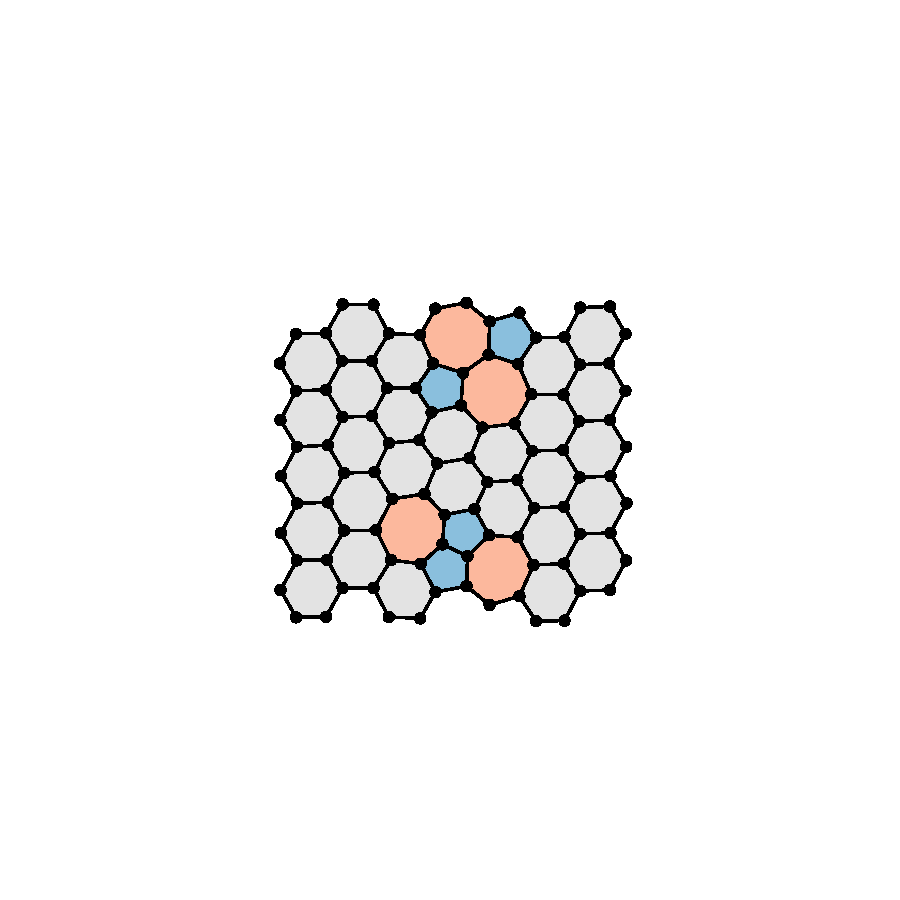
\includegraphics[height=2.8cm]{./figures/methods/bs_t2.pdf}
         \caption{}
         \label{fig:bsmc8}
     \end{subfigure}
   
     \caption{Configurations taken from stages of the \td{} bond switching algorithm. A crystalline lattice (a) is first thermalised to generate a random high energy network (f) by sequential overlapping Stone\--Wales defects (b)-(e). Sampling then occurs as the system is slowly annealed (g)-(h), allowing access to defect states that are not initially obtainable from the crystal structure.}
     \label{fig:bsmc}    
\end{figure}
The \mc{} move for 3\--coordinate atomic materials is essentially the introduction of a Stone\--Wales defect into the lattice, which
augments the size of two rings and decrements two others, preserving both the mean ring size and the coordination number of the individual atoms involved in the transformation \cite{Stone1986}.
As defects become more concentrated they overlap, leading to increasing diversity into the ring structure (allowing access to more than the pentagons and heptagons in a single Stone\--Wales defect).
Each bond transposition is followed by geometry optimisation to minimise and calculate the total energy of the system.  
A key aspect in the bond switching algorithm is therefore the choice of potential model.
The potential models and geometry optimisation process used in this thesis can be found in subsections below.

Cooling the system slowly ensures that the material remains in thermodynamic equilibrium, allowing configurations to be sampled throughout the simulation.
The ring structure of the system is then related to the temperature parameter, with more extreme ring sizes appearing at higher temperatures (compare figure \ref{fig:bsmc6}\--\ref{fig:bsmc8}).
This simply reflects the inherent balance of enthalpic \vs{} entropic  considerations.
Figure \ref{fig:bsmc8} also demonstrates the importance of cooling a randomised lattice instead of heating a crystal, as some low energy defects may have a multi\--step formation with a high energy barrier.  

\subsection{Potential Models}
\ref{s:potentials}

The nature of the bond switching method lends itself to the use of semi\--empirical potentials which have explicit stretching and angular neighbour lists.
As such a popular choice for materials modelling is the Keating potential and modifications thereof \cite{Keating1966,Barkema2000}. 
For a \td{} system the Keating potential has the form:
\begin{equation}
	\label{eq:keating}
	\pen = \frac{3}{16}\frac{\fk_S}{r_0^2}\sum_{\substack{i,j \in \\ \text{stretches}}} \left(r_{ij}^2-r_0^2\right)^2+
	\frac{3}{8}\frac{\fk_A}{r_0^2}\sum_{\substack{ijk \in \\ \text{angles}}}\left(r_{ij}r_{ik}\cos\theta_{ijk}-r_0^2\cos\theta_0\right)^2 \,,
\end{equation}
where $r_{ij}$ the distance and $\theta_{ijk}$ the angle between particles; whilst $\fk_S$ and $\fk_A$ are the force constants for the stretching and angular terms respectively \cite{Kumar2012}.
This potential drives the system towards equilibrium values of $r_0$ for the bond lengths and $\theta_0$ for the bond angles.
The Keating potential has been parametrised for a range of specific materials \cite{Kumar2012,Drabold2009}. 

However, a more generic potential model is sometimes required which captures the same essential physics.
This is provided through the simplified Keating potential \cite{VonAlfthan2003},
\begin{equation}
	\pen = \frac{\fk_S}{2}\sum_{\substack{i,j\in \\ \text{stretches}}}\left(r_{ij}-r_0\right)^2 + \frac{\fk_A}{2}\sum_{\substack{i,j,k \in \\ \text{angles}}} \left(\cos\theta_{ijk}-\cos\theta_0\right)^2\,,
\end{equation}
which is harmonic in stretching and angular terms.
One final modification can be made to this potential. 
Sometimes it is informative build models which enforce ring convexity \ie{} maintain all angles within the range $0\leq \theta_{ijk} \leq \pi$.
This can be achieved by augmenting the simplified Keating potential with a restricted bending (ReB) potential \cite{Bulacu2013}:
\begin{equation}
	\pen = \frac{\fk_S}{2}\sum_{\substack{i,j\in \\ \text{stretches}}}\left(r_{ij}-r_0\right)^2 + \frac{\fk_A}{2}\sum_{\substack{i,j,k \in \\ \text{angles}}} \frac{\left(\cos\theta_{ijk}-\cos\theta_0\right)^2}{\sin^{2}\theta_{ijk}}\,.
\end{equation}
The addition of the sine term in denominator causes the potential to diverge as bond angles approach linearity, preventing bonds from ``inverting''.

\subsection{Geometry Optimisation}
\label{s:geomopt}

The purpose of geometry optimisation is to minimise the overall potential energy of a network, $\pen$, as a function of all atomic positions, $\mathbf{r}$, after they have been perturbed \eg{} by a bond transposition.
As all initial configurations are well relaxed and perturbations relatively small, this can be achieved with a local minimisation routine.
In addition as the potential models in this work are smooth and harmonic, a straightforward steepest descent algorithm is both sufficient and efficient.

The steepest descent algorithm is an iterative method which searches down the potential energy gradient until a minimum is reached \cite{Nocedal2006}.
It has the following scheme:
\begin{enumerate}
	\item Calculate the potential energy of the system $\mathcal{U}_i=\mathcal{U}\left(\mathbf{r}_i\right)$
	\item Determine the negative gradient of the potential \ie{} the forces acting on the particles $\mathbf{F}_i=-\nabla \mathcal{U}_i$ 
	\item Find the optimal distance to displace the particles along the lines of force $\mathcal{U}_{i+1}=\min \left[\mathcal{U}\left(\mathbf{r}_i+\lambda \mathbf{F}_i\right)\right]$
	\item Set $\mathbf{r}_{i+1}=\mathbf{r}_i+\lambda_{\text{min}} \mathbf{F}_i$
	\item Evaluate convergence and repeat steps 1-4 if $\left|\mathcal{U}_{i+1}-\mathcal{U}_i\right|>\gamma$
\end{enumerate}
The calculation of forces in stage 2 will depend on the potential model used, details of which are given in appendix \ref{app:forces}.
Note that stage 3 also requires a minimisation routine, which may seem counter\--intuitive. 
However, this is a one\--dimensional minimisation which trivial to estimate with a line search method \davidnote{appendix?}.
The tightness of the convergence condition is set through the parameter $\gamma$.

One final performance improvement arises from the fact that the \mc{} are inherently local.
Therefore geometry optimisation can be employed such that only the atoms in the immediate vicinity of the switching move need to be minimised to obtain an accurate structure.
Typically this would extend to all atoms within five coordination shells of those directly involved in the switch move \cite{Mousseau2001}.

\section{Hard Particle \mc}
\label{s:hardparticlemc}

Hard particle Monte Carlo is one of the most well\--established computational methods in statistical physics.
Through its simplicity it is able to provide insight into the fundamental behaviour of particle systems and simulations of increasing size are still performed this century \cite{Isobe2016,Bernard2009,Anderson2013,Isobe2015}.
In this thesis it will be used to generate ring systems in the form of Voronoi tessellations (see section \ref{ssec:voronoi}), in analogy to experimental colloidal systems \cite{Thorneywork2017}.

\subsection{Hard Particle Model}

Hard particle models are applicable over a range of dimensions.
In two dimensions the system consists of an arrangement of hard disks and in three dimensions hard spheres.
One can also take a quasi \td{} system, which comprises hard spheres confined to a plane.
Regardless of the dimensionality, the central principle is that no two particles in the system can have any degree overlap.
Formally, if the particle radii are denoted by $R_i$ and the distance between any pair of particle centroids by $r_{ij}$, the pair potential is:
\begin{equation}
	\mathcal{U}_{ij} = \begin{cases}
	\infty \quad &r_{ij}<R_i+R_j \\
	0 \quad &r_{ij}\geq R_i+R_j 
	\end{cases} \,.
\end{equation}
As the total energy is simply then
\begin{equation}
	\pen = \sum_{i<j} \mathcal{U}_{ij}\,,
\end{equation}
it follows that if any pair of particles have overlap the system energy is infinite and the Boltzmann weighting is zero.
Hard particle models are typically quantified in terms of the packing fraction, $\phi$, which in two dimensions has the form
\begin{equation}
	\label{eq:packingfraction}
	\phi_{2D} = \rho\pi\langle R^2\rangle\,,
\end{equation}
where $\rho=\mathcal{N}/{V}$, the number density.

\subsection{Algorithmic Details} 

\begin{figure}[bt]
     \centering
     
     \begin{subfigure}[b]{0.25\textwidth}
         \centering
         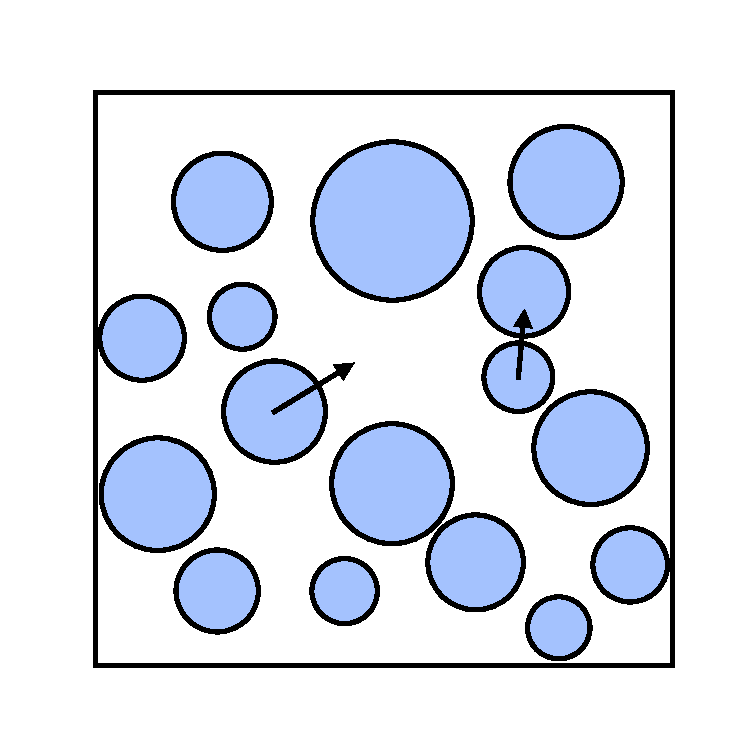
\includegraphics[width=3cm]{./figures/methods/mc_move_a.pdf}
         \caption{}
         \label{fig:hardmc1}
     \end{subfigure}
     \begin{subfigure}[b]{0.25\textwidth}
         \centering
         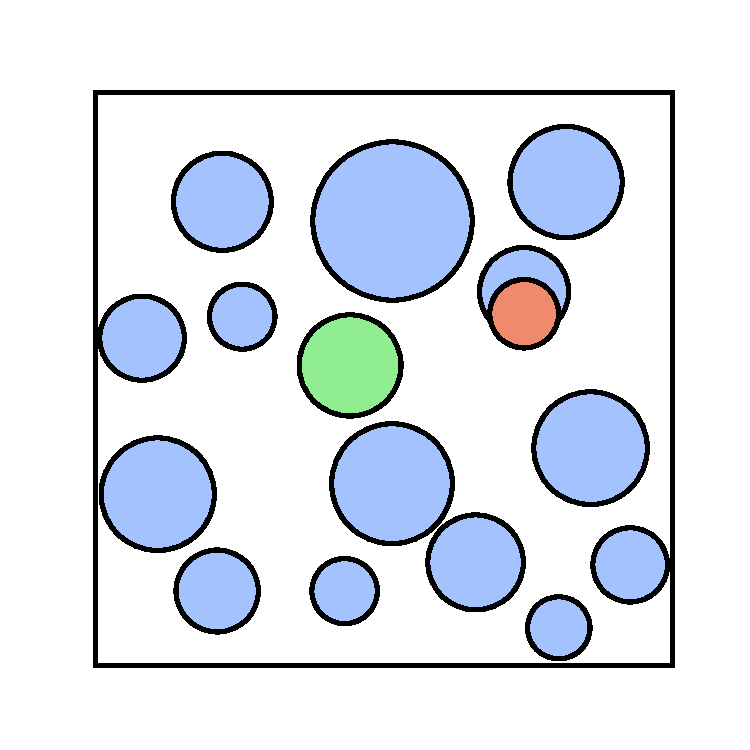
\includegraphics[width=3cm]{./figures/methods/mc_move_b.pdf}
         \caption{}
         \label{fig:hardmc2}
     \end{subfigure}
     \begin{subfigure}[b]{0.25\textwidth}
         \centering
         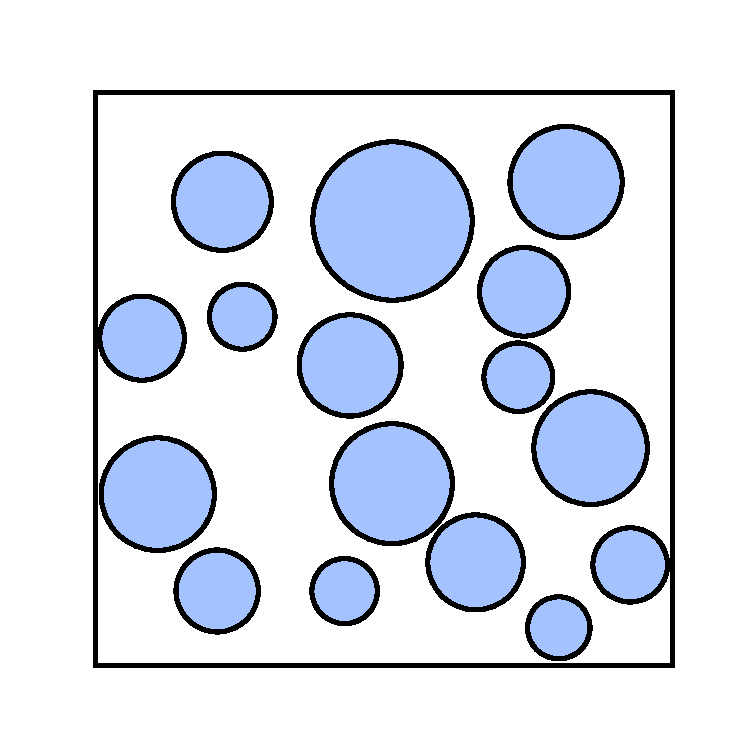
\includegraphics[width=3cm]{./figures/methods/mc_move_c.pdf}
         \caption{}
         \label{fig:hardmc3}
     \end{subfigure}
     
       \begin{subfigure}[b]{0.25\textwidth}
         \centering
         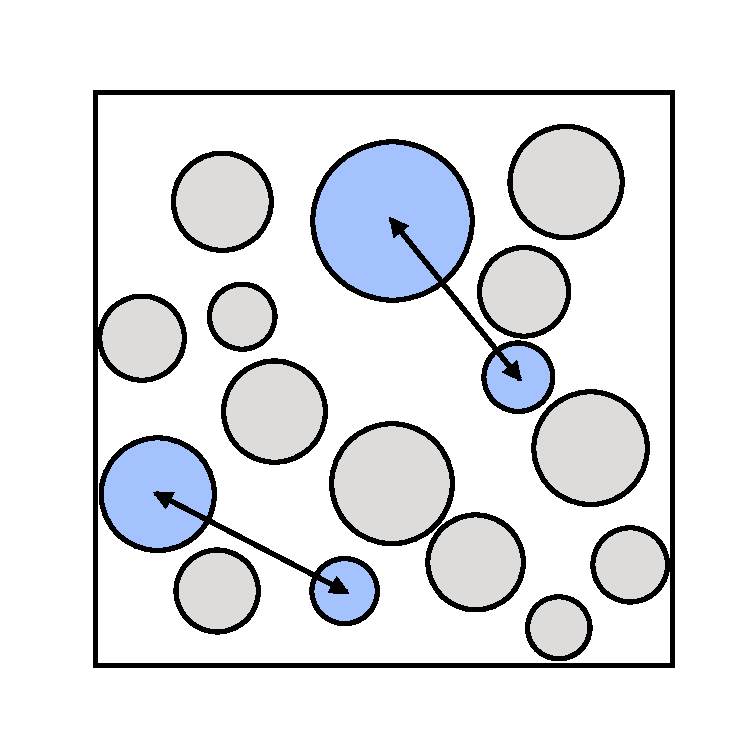
\includegraphics[width=3cm]{./figures/methods/mc_move_d.pdf}
         \caption{}
         \label{fig:hardmc4}
     \end{subfigure}
     \begin{subfigure}[b]{0.25\textwidth}
         \centering
         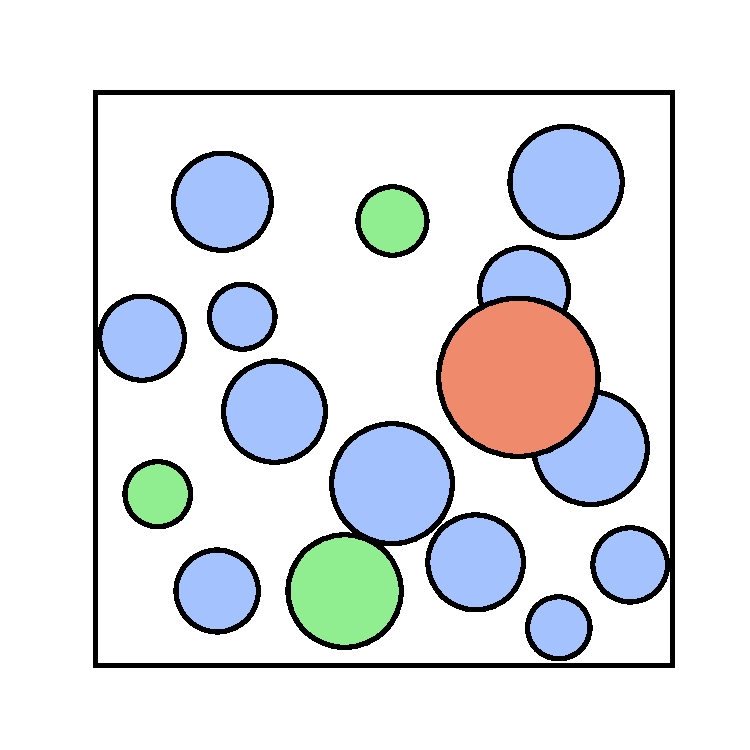
\includegraphics[width=3cm]{./figures/methods/mc_move_e.pdf}
         \caption{}
         \label{fig:hardmc5}
     \end{subfigure}
     \begin{subfigure}[b]{0.25\textwidth}
         \centering
         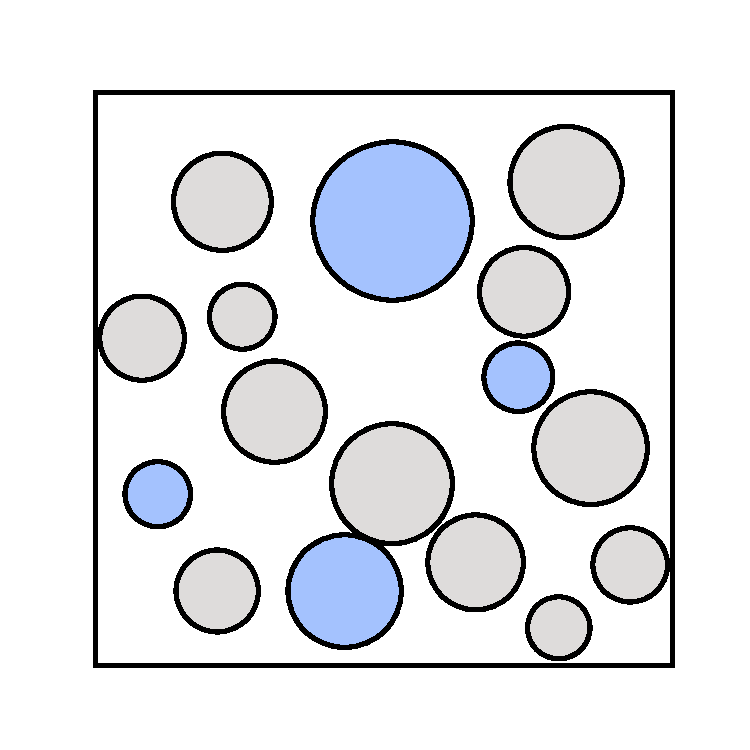
\includegraphics[width=3cm]{./figures/methods/mc_move_f.pdf}
         \caption{}
         \label{fig:hardmc6}
     \end{subfigure}
   
     \caption{Demonstration of two displacement (a)\--(c) and two swap (d)\--(f) moves in hard particle \mc.
     In displacement moves, particles are randomly selected and assigned a trial random displacement vector (a). In swap moves, two particles are randomly selected and their radii trial swapped (b). The trial move is then examined to see if it introduces any particle overlaps (b),(e). If there are no overlaps (green), then the trial move is accepted and the system updated but otherwise (red) the move is rejected and the system returns to the previous state (c),(f).
     }
     \label{fig:hardmc}
     
	\vspace{1cm}
	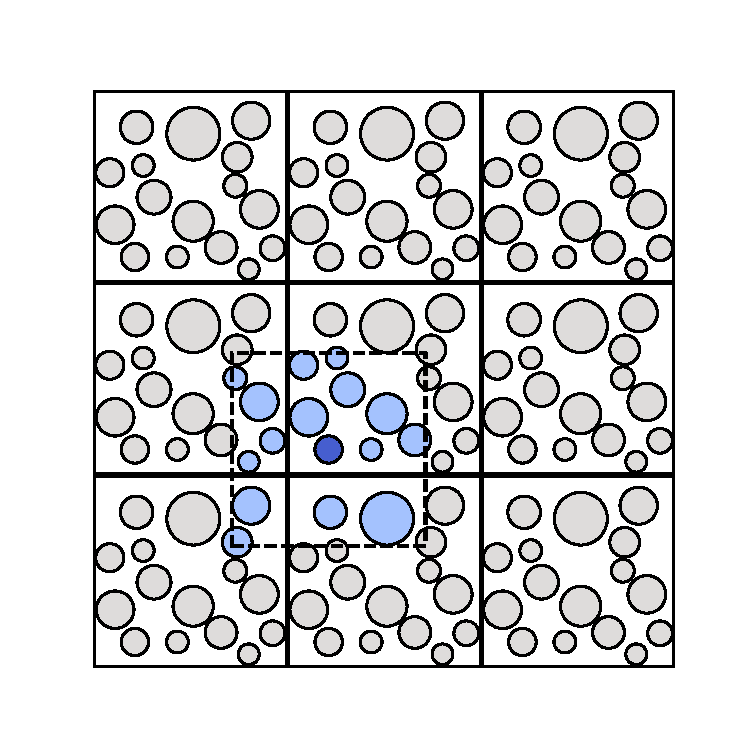
\includegraphics[width=5cm]{./figures/methods/mc_move_g.pdf}
	\caption{Simulation of bulk system is achieved using periodic boundary conditions, where a central cell is surrounded by repeated images of itself. A particle of interest (dark blue) then interacts with the nearest images of every other particle (light blue).}
	\label{fig:pbc}     
\end{figure}

Hard particle systems can be simulated using the Metropolis algorithm outlined in section \ref{ssec:metropolis}.
The system is initialised by selecting a random non\--overlapping configuration.
This can be achieved easily for low to medium densities by a greedy algorithm like random sequential addition, where particles are added successively in a manner which does not overlap with any previous particles \cite{Widom1966}.
For higher packing fractions a more sophisticated algorithm is needed \davidnote{Find refs}.

Once the initial configuration has been generated, it is evolved via two \mc{} moves.
The first is the displacement move, whereby a random particle is selected and translated according to a random vector with elements generated uniformly in the range $\left[-\delta,\delta\right]$.
If the displacement introduces any particle overlaps it is rejected, otherwise the system is updated to the new configuration, as illustrated in figure \ref{fig:hardmc1}\--\ref{fig:hardmc3}.
The value of $\delta$ is chosen for each simulation such that the proportion of accepted moves is $\sim 50\%$, allowing for efficient searching of configurational space.
The optimal value can be determined by continuous adjustment during equilibration.

The second is the swap move, where two random particles are selected their radii exchanged \cite{Grigera2001,Ninarello2017}. 
Once again a swap move is only accepted if it does not lead to any overlapping particles and is demonstrated in figure \ref{fig:hardmc4}\--\ref{fig:hardmc6}.
The swap move is used to increase the efficiency in simulations of polydisperse particles and is an example of how the design of \mc{} moves can be flexible and they do not have to have a direct physical basis. 
The swap move is attempted for every ten displacement moves. 

Finally, to remove the presence of an interface in the system, simulation is performed with periodic boundary conditions.
In this scheme the central simulation cell is repeated to form an infinite lattice, so that every particle experiences a bulk environment.
Coupled with this is the use of the minimum image convention, where each particle then only interacts with the nearest repeated image of all the remaining particles.
This is illustrated in figure \ref{fig:pbc}.
 
\subsection{Voronoi Construction}
\label{ssec:voronoi}


The hard particle configurations produced by \mc{} simulations are not in themselves network structures, rather simply a collection of correlated points.
The network structure is revealed by construction of a Voronoi diagram, which partitions the sample into a system of tessellating cells, where each cell encapsulates all the space closest to the associated particle \cite{Okabe1992}.
A \td{} Voronoi diagram is formed through the placement of dividing lines between the centroids of neighbouring particles. 
The intersection of these lines forms the characteristic tessellating polygons.

\begin{figure}[bt]
     \centering
     
     \begin{subfigure}[b]{0.22\textwidth}
         \centering
         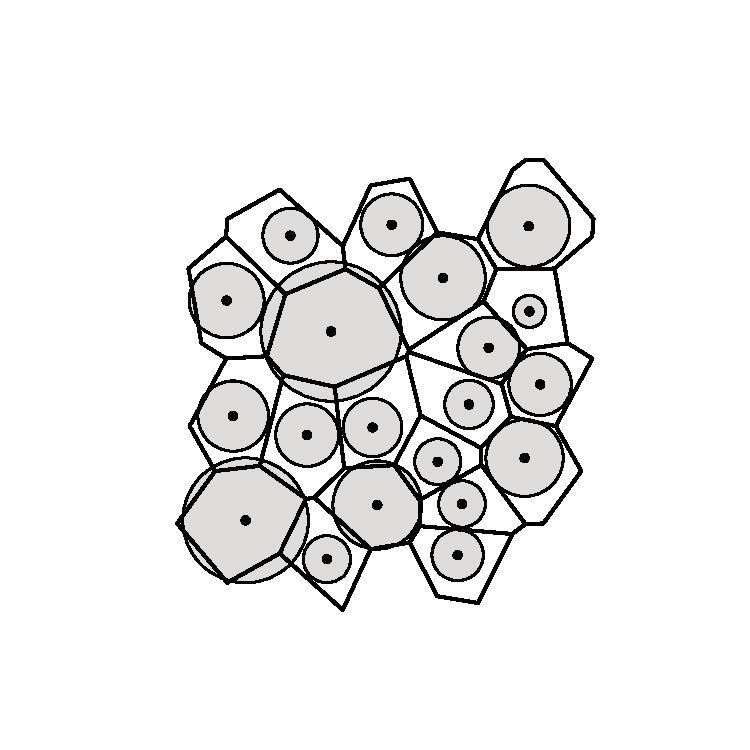
\includegraphics[width=\textwidth]{./figures/methods/voro_demo_vw.pdf}
         \caption{}
         \label{fig:vorodemov1}
     \end{subfigure}
     \hfill
     \begin{subfigure}[b]{0.22\textwidth}
         \centering
         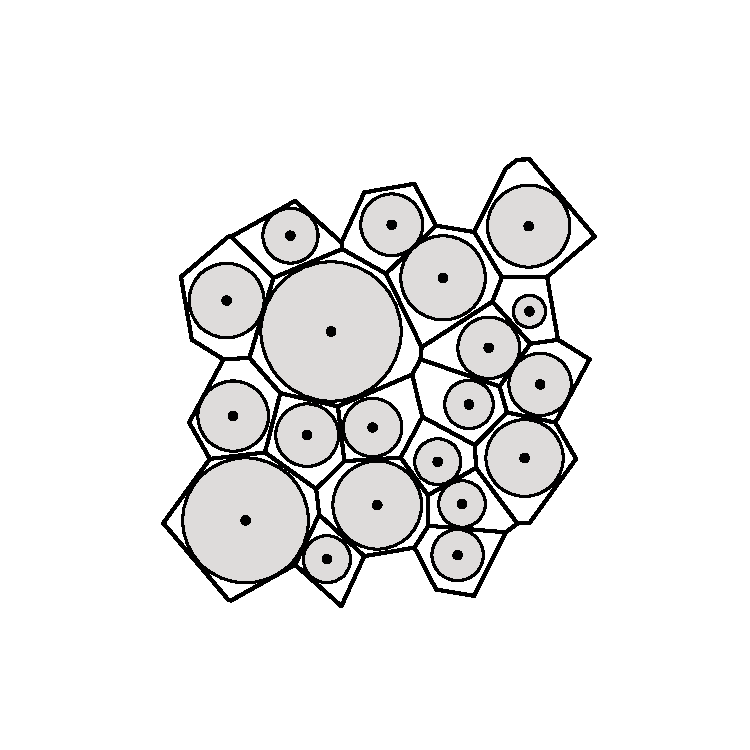
\includegraphics[width=\textwidth]{./figures/methods/voro_demo_rw.pdf}
         \caption{}
         \label{fig:vorodemor1}
     \end{subfigure}
     \hfill
     \begin{subfigure}[b]{0.22\textwidth}
         \centering
         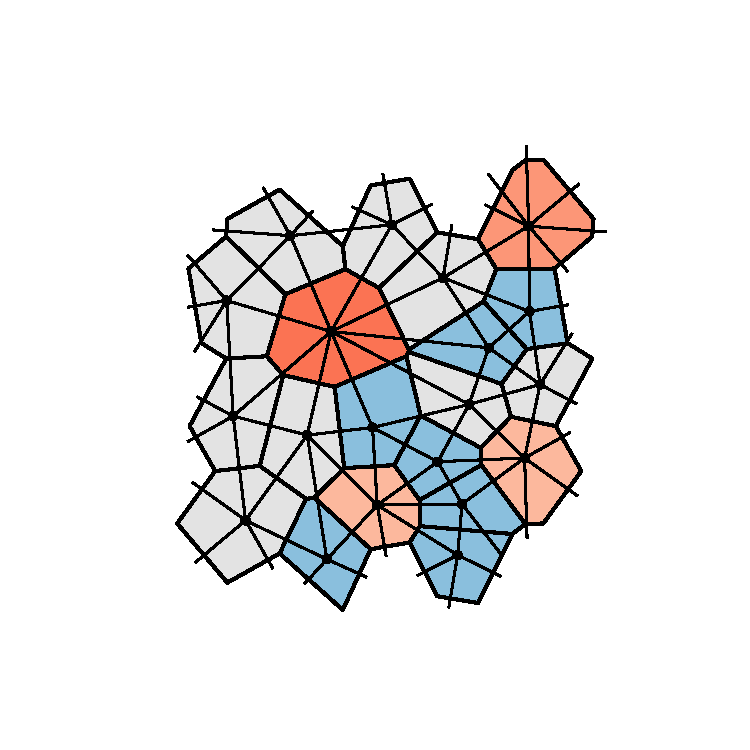
\includegraphics[width=\textwidth]{./figures/methods/voro_demo_vcd.pdf}
         \caption{}
         \label{fig:vorodemov2}
     \end{subfigure}
     \hfill
       \begin{subfigure}[b]{0.22\textwidth}
         \centering
         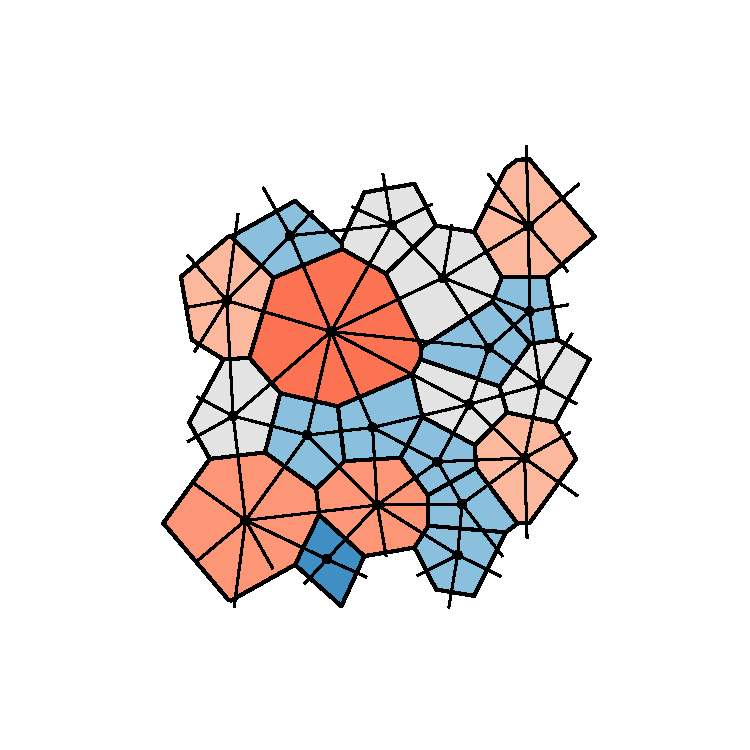
\includegraphics[width=\textwidth]{./figures/methods/voro_demo_rcd.pdf}
         \caption{}
         \label{fig:vorodemor2}
     \end{subfigure}
   
     \caption{Voronoi construction of a polydisperse hard disk system. Panels (a) and (b) compare the unweighted and weighted (radical) Voronoi tessellations respectively. The radical Voronoi assigns more volume to the larger particles to ensure a more equitable distribution of space, which can affect the underlying ring structure, shown in panels (c) and (d). The dual network, known as the Delaunay triangulation, is also overlaid.}
     \label{fig:vorodemo}
\end{figure}

In the simplest unweighted approach, the dividing line between two neighbouring particles separated by the Euclidean distance $r_{ij}$, is simply located midway between the particles at a distance $r_{ij} /2$. 
The elegance of the unweighted Voronoi diagram is that only the particle centroids are required for its construction, with no requirement for a cut-off parameter. 
Whilst the unweighted Voronoi tessellation is very effective for studying monodisperse particles, there are some limitations for polydisperse species. 
Specifically, the Voronoi partition underestimates the space assigned to large particles and overestimates that for small particles \-- a simple reflection of the lack of information on particle radii  (see figure \ref{fig:vorodemov1}). 
To rectify this, weighted modifications have been suggested which take account of the differences in radii \cite{Poupon2004}.

To construct a weighted Voronoi diagram, one simply adjusts the position of the dividing line, such that it is further from the particle with the greater weight. 
The weighting method used in this work is the so called radical tessellation introduced by Finney \cite{GELLATLY1982}. In this modification, the dividing line is placed a distance $d_i$ from particle $i$, given by:
\begin{equation}
	\label{eq:radical}
	d_i = \frac{w_i^2-w_j^2+r_{ij}^2}{2r_{ij}}\,,
\end{equation}
where $w_i$ and $w_j$ are the weights for each particle. 
The benefit of this method is that is adjusts the partitioning of space so that greater volume is assigned to the particles with larger weight, and is well designed so that all of the sample space remains accounted for - unlike some alternative constructions \cite{Richards1974}. 
In terms of the particle weights, the logical choice is simply the disk radii. 
This is because at the contact distance, $r_{ij} = R_i + R_j$, equation \eqref{eq:radical} shows that $d_i = R_i$ \ie{} the radical dividing line sits exactly between the two disks, producing the most equitable distribution of volume (see figure \ref{fig:vorodemor1}). 
Furthermore, when the radii are equal, $d_i = r_{ij} /2$ and the result from the standard unweighted Voronoi is regenerated as expected.
It is worth noting here that the weighting method can affect the ring sizes (\ie{} number of vertices) as well as the ring areas, as demonstrated in figures \ref{fig:vorodemov2},\ref{fig:vorodemor2}.

The outcome of the Voronoi construction is a system of percolating rings not dissimilar to those seen in materials.
The dual network, known as the Delaunay triangulation, is also obtained, which defines the nearest neighbours for each particle.
The main difference with atomic materials is that the polygon edge lengths and angles are not constrained by a potential model the ring structure is therefore completely entropically controlled.
The degree of disorder is then determined by the packing fraction, $\phi$, where decreasing the packing fraction leads to increased diversity in the ring statistics, as illustrated in figure \ref{fig:voromono}.
As can be seen there are some defects which are analogous to those seen in materials, such as the Stone\--Wales defect in figure \ref{fig:voromono2}, but others are not, as in figure \ref{fig:voromono1} which arise from very small perturbations in the crystalline lattice.
The limiting value as $\phi\rightarrow 0$ is well studied as the Poisson Voronoi diagram \cite{Boots1983,Tanemura2003}.
This corresponds to the Voronoi diagram formed from a random uniform array of points.
In this way Voronoi systems provide a good complement to compare and contrast with materials.

\begin{figure}[bt]
     \centering
          \begin{subfigure}[b]{0.24\textwidth}
         \centering
         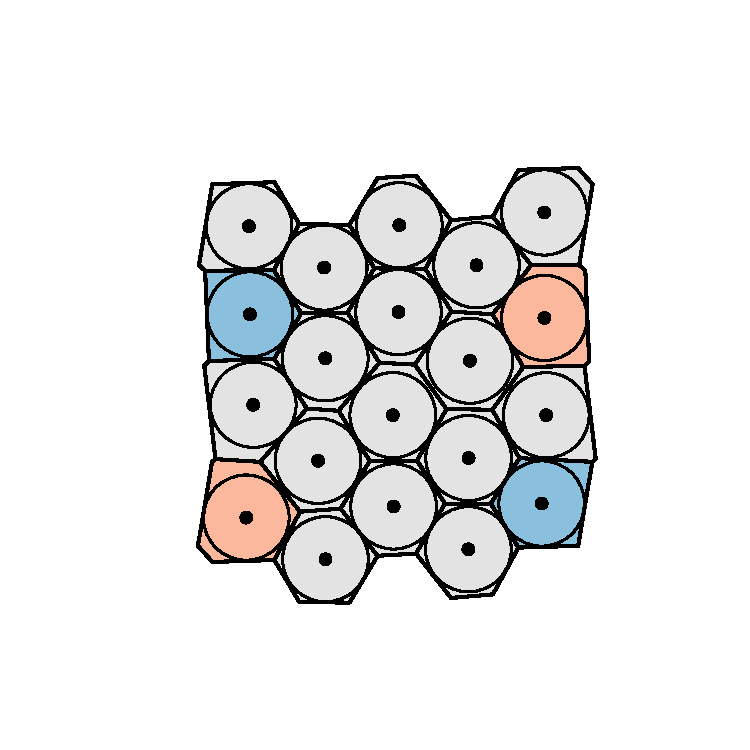
\includegraphics[height=3cm]{./figures/methods/voro_mono_80.pdf}
         \caption{$\phi=0.8$}
         \label{fig:voromono1}
     \end{subfigure}
     \hfill
     \begin{subfigure}[b]{0.24\textwidth}
         \centering
         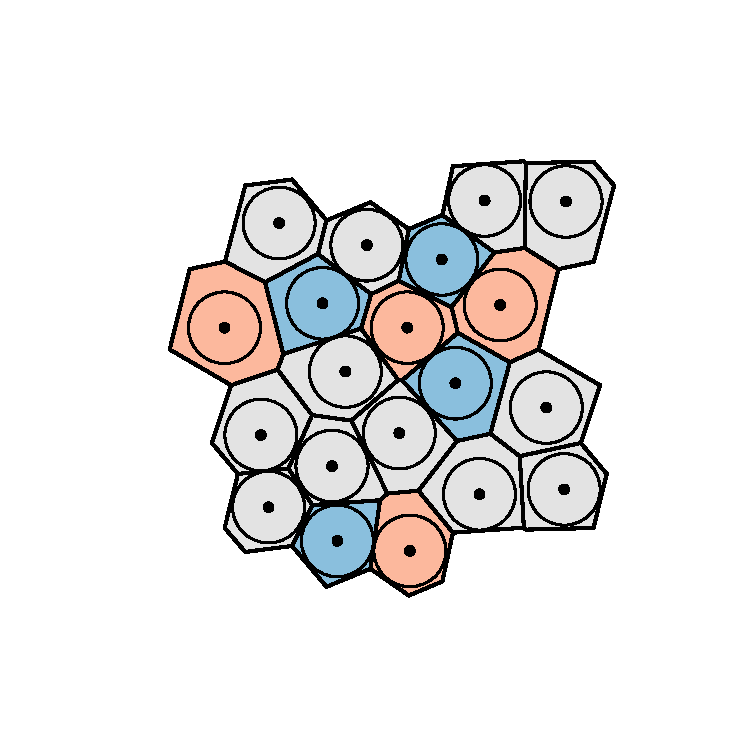
\includegraphics[height=3cm]{./figures/methods/voro_mono_60.pdf}
         \caption{$\phi=0.6$}
         \label{fig:voromono2}
     \end{subfigure}
     \hfill
     \begin{subfigure}[b]{0.24\textwidth}
         \centering
         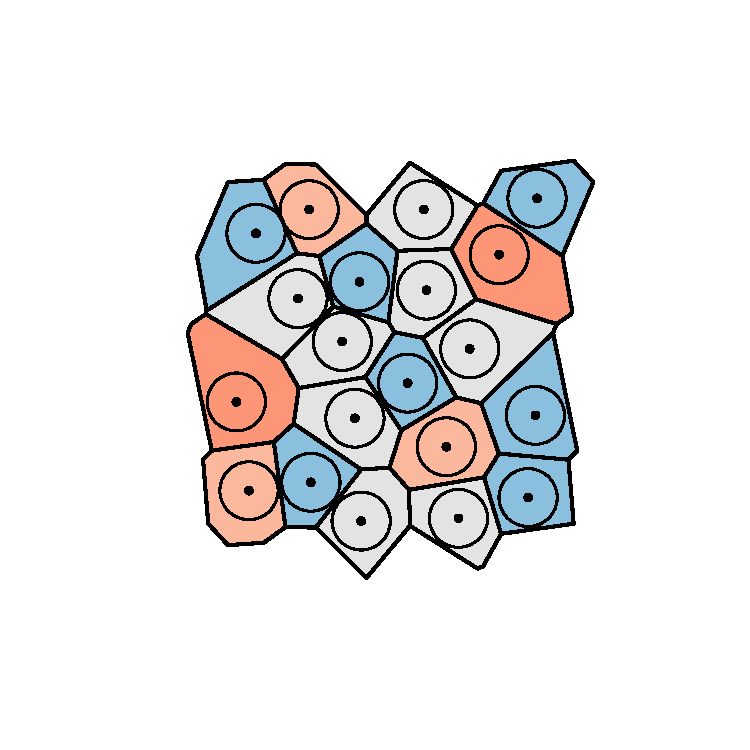
\includegraphics[height=3cm]{./figures/methods/voro_mono_40.pdf}
         \caption{$\phi=0.4$}
         \label{fig:voromono3}
     \end{subfigure}
     \hfill
       \begin{subfigure}[b]{0.24\textwidth}
         \centering
         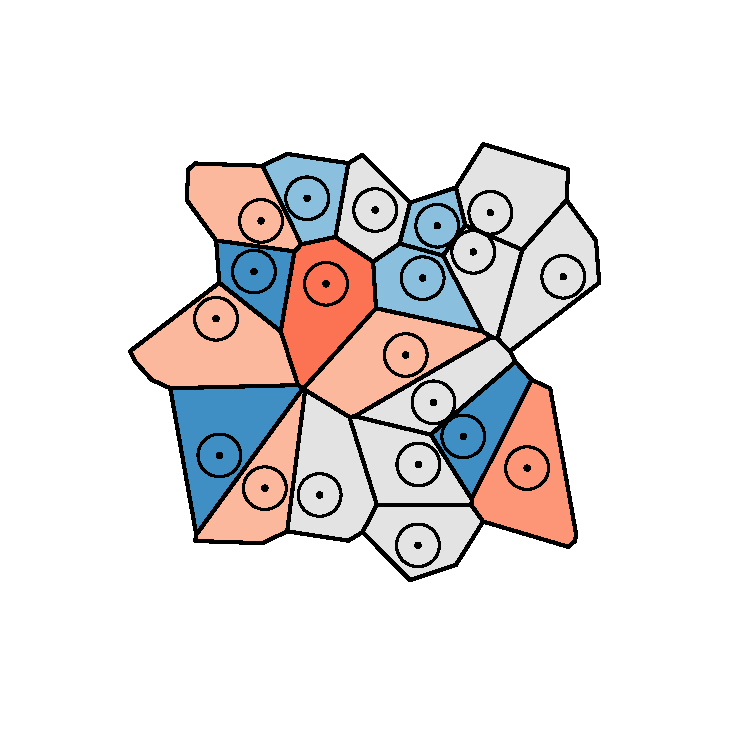
\includegraphics[height=3cm]{./figures/methods/voro_mono_20.pdf}
         \caption{$\phi=0.2$}
         \label{fig:voromono4}
     \end{subfigure}
     \caption{The ring structure in Voronoi diagrams is controlled through the packing fraction, $\phi$, of the underlying hard particle system. Ring diversity increases as packing fraction is lowered from $0.8\rightarrow 0.2$ in (a)\--(d).}
     \label{fig:voromono}
\end{figure}

\section{Analysis Methods}

\subsection{Bond Length and Angle Distributions}

\subsection{Radial Distribution Functions}







%\chapter[Modelling Bilayer Materials]{Modelling Bilayer Materials}
\label{ch:bilayers}

\begin{chapterabstract}
A computationally tractable \mc{} method using triangle rafts is developed to generate bilayers of \sioii{} and related materials.
The method allows defect free networks of any given shape to be grown with both tuneable ring statistics and topologies, controlled by a combination of the ``allowed'' rings and the effective growth ``temperature''. 
Configurations are generated with \aw{} parameters commensurate with those obtained from an analysis of experimental configurations, improving significantly on previous methods.
The ability to efficiently grow configurations allows exploration of the structural basis of \lm’s law, where the commonly observed value of $p_6\approx0.4$ is presented as a balance between entropic and enthalpic factors. 
The deviations of ring areas from the ideal values are discussed and the relative insensitivity of the ring area to relatively strong distortions is highlighted.
\end{chapterabstract}

\section{Bilayer Materials}

An important class of \td{} materials which have emerged in the 21\st{} century are bilayers of silica, \sioii, and related species \cite{Buchner2017}.
These can be prepared experimentally by chemical vapour deposition on metal and graphene supports \cite{Huang2012,Lichtenstein2012a}.
As in the three\--dimensional glass, the basic building blocks of silica bilayers are vertex sharing \sioiv{} tetrahedra, maintaining full coordination for all atoms in the bulk \cite{Wilson2013}.
These are arranged such that three of the vertices are connected to tetrahedra in the same layer, with the final vertex being shared between layers acting as a ``bridge'' (figure \ref{fig:bilayer1}).
A consequence of these bridging oxygen atoms is to enforce a symmetry plane between the upper and lower layers.

Topologically, the symmetry plane means that these materials can be viewed as effective \td{} networks.
Taking one of the layers, without the bridging oxygens, and projecting the atoms onto the horizontal plane reveals a representation of vertex sharing triangles, referred to as a triangle raft (figure \ref{fig:bilayer2}).
The ring structure then emerges from the three\--coordinate network formed by connecting the silicon atoms of adjacent triangles as in figure \ref{fig:bilayer3}.
Indeed, scanning tunnelling microscopy (STM) has been used to directly visualise the ring structure in silica bilayers, revealing both crystalline and glassy arrangements and even the interface between the two   \cite{Loffler2010,Lichtenstein2012b}.

More recently experimentalists have also succeeded in synthesising bilayers of germania, \geoii{} \cite{Lewandowski2018,Lewandowski2019}.
\davidnote{Add a bit more experimental context here, discuss with Mark}
%These have the same fundamental structure as \sioii{}, but with more distorted tetrahedra \davidnote{Why again...some inorganic stuff...}.
%This can lead to a build up of strain and rumpling of the tetrahedral layers.
%\marknote{Have you discussed somewhere why they are doing this? Control of the pore size and pote
%density critical for gas separation applications....}
%\marknote{Note somewhere that making the GeO2 analogue is more difficult experimentally.....}

\begin{figure}[bt]
     \centering
     
     \begin{subfigure}[b]{0.3\textwidth}
         \centering
         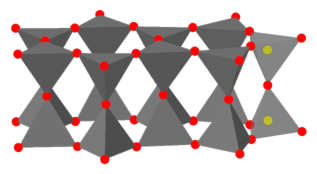
\includegraphics[width=\textwidth]{./figures/bilayers/mx2_bilayer_1.pdf}
         \vspace{-1mm}
         \caption{Tetrahedral bilayer}
         \label{fig:bilayer1}
     \end{subfigure}
     \hfill
	\begin{subfigure}[b]{0.3\textwidth}
         \centering
         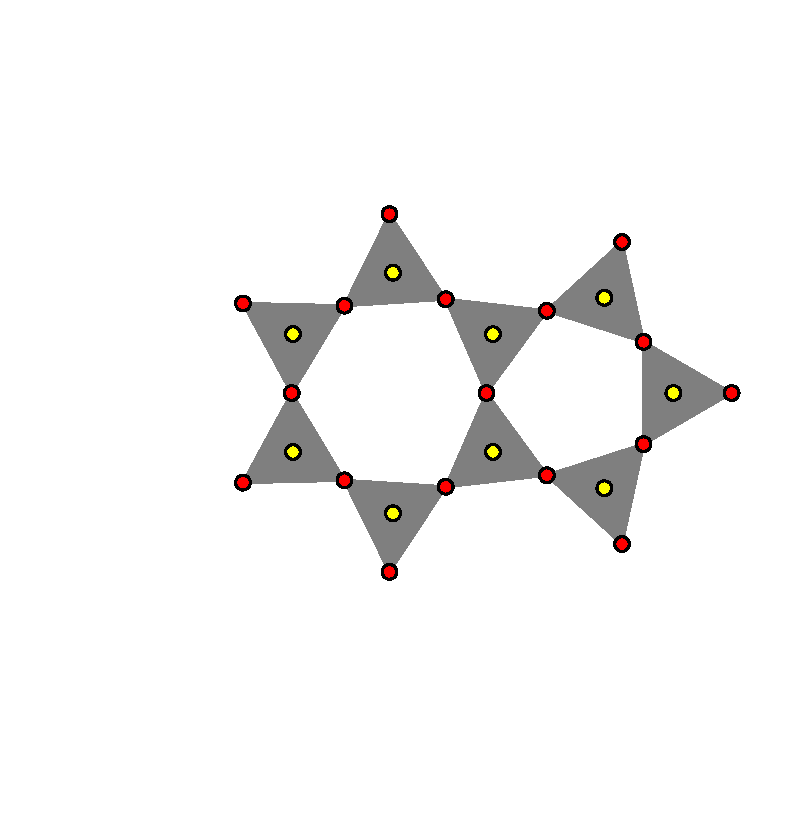
\includegraphics[width=\textwidth]{./figures/bilayers/mx2_bilayer_2.pdf}
         \caption{Triangle raft}
         \label{fig:bilayer2}
     \end{subfigure}
     \hfill
     \begin{subfigure}[b]{0.3\textwidth}
         \centering
         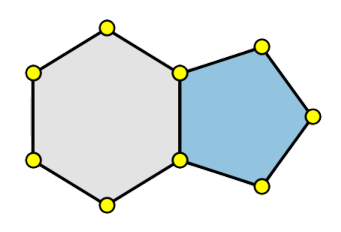
\includegraphics[width=0.8\textwidth]{./figures/bilayers/mx2_bilayer_3.pdf}
         \vspace{5mm}
         \caption{Ring structure}
         \label{fig:bilayer3}
     \end{subfigure}
     \hfill
     
     \caption{Silica bilayers of vertex sharing tetrahedra in (a) can be represented as a \td{} triangle raft in (b). Silicon and oxygen atoms are coloured yellow and red respectively. The ring structure then emerges from the three\--coordinate network comprising the silicon atoms, (c).}
     \label{fig:bilayer}
\end{figure}

\section{Review of Existing Methods}
\label{s:triraftexisting}

As mentioned in the  introduction, both \abinitio{} methods and classical molecular dynamics have been used in computational studies of silica bilayers, which often require a starting atomistic configuration  \cite{Bjorkman2013,Malashevich2016,Wilson2013,Roy2018}.  
One approach is to simply take an experimental sample as the starting structure. 
Whilst this may be on the surface the best solution, the experimental configurations may contain defects or areas where the image is corrupted \ie{} the configuration may not be ``pristine''.
Additionally, the location of each atom has an associated uncertainty which leads to discrepancies in the observed bond lengths and angles, which can be compounded by any out\--of\--plane distortions.
Whilst computational refinement can attenuate these problems \cite{Sadjadi2017,Wilson2018}, there remains the more fundamental question of how ``typical'' the available images are from experiment, as STM provides exceptional information but only on relatively small sample sizes.
Computational techniques can therefore prove a valuable tool for generating a large number of high\--quality configurations and corroborating experimental information.  

One current approach is to transform amorphous graphene configurations \cite{Wilson2013}.
Here amorphous samples of carbon are generated using a bond switching method (as outlined in section \ref{s:bondswitch}), before the carbon atoms are swapped from silicon and decorated with oxygens.
Whilst this is a valid approach, the method assumes that the two materials are topologically equivalent.
This is likely an oversimplification, as the presence of the bridging oxygens in silica afford the structure increased flexibility when compared to the carbon analogue.
This likely explains why this method has struggled to mirror experimentally observed values of the ring statistics and \aw{} parameter, with small and large ring proportions being under\--estimated \cite{Kumar2014}.

An alternative approach is to use molecular dynamics coupled with an effective pair potential to obtain viable configurations \cite{Roy2018}.
Such methods are relatively common, having been employed previously to study amorphous graphene \cite{Kumar2012}. 
Such methods offer the potential for generating realistic configurations but are difficult to control as the cooling rates which must be applied are necessarily huge compared to experimental rates. 
A potential artefact of the high cooling rates is the effectively freezing in of defect states, either in terms of local coordination environments or highly\--strained (three-membered) rings.
In addition, as with the method above, such methods appears to systematically underestimate the \aw{} parameter, indicative of too little structural ordering.

\section{Triangle Raft Method}
\label{s:triangleraft}

The motivation of this work was to develop a construction algorithm to generate samples of silica bilayers which can capture the full \td{} network topology; both the ring distribution \textit{and} correlations. 
The model should be able to explore all phases from crystalline to amorphous yet computationally efficient enough to produce configurations suitable for further high throughput calculations. 
To achieve this a grow-from-seed Monte Carlo algorithm has been developed, where rings are individually added to build a triangle raft.
This approach takes inspiration from the first hand\--built models, which have been noted to bear close resemblance to experimental structures \cite{Shackelford1982a,Buchner2016a}.
Such models were superseded by computational techniques designed to generate periodic configurations. 
However, the recent development in techniques to simulate aperiodic samples, such as sliding boundary conditions for molecular dynamics \cite{Theran2015}, makes this constraint no longer essential, and benefit may be gained from the added freedom of an aperiodic model.


\subsection{Potential Model}

As explained in figure \ref{fig:bilayer} it is possible to capture the full topology of silica bilayers with a simplified representation consisting of a network of vertex\--sharing \sioiii{} triangles. 
As the focus of this chapter is on generating a large number of samples with varying ring statistics, %to be used as a base for further calculations, 
working with this reduced representation is sufficient, as it provides a computationally efficient way to produce networks with the required \textit{topology}. 
The precise \textit{geometry} of the bilayer can be refined with advanced optimisation techniques if required \cite{Tangney2002}. 

In order to simulate bilayer systems in two dimensions, a suitable potential model is needed which captures the essential physics of the system: the local triangular environment of the \sioiii{} units and the relative energies of rings of different sizes. 
The model used here is modified from a relatively simple potential used in all\--atom bilayer calculations \cite{Wilson2013,Wilson2018}, a schematic for which is given in figure \ref{fig:trpotmodel}.
Each \sioiii{} unit has a harmonic potential acting between all three Si\---O pairs, and the three nearest\--neighbour O\---O pairs, given by:
\begin{equation}
	\label{eq:harmonic}
	\mathcal{U}_{ij} = \frac{\fk}{2}\left(r_{ij}-r_{ij}^{0}\right)^{2},
\end{equation}
where $\fk$ is a constant, $r_{ij}$ is the interatomic separation and $r_{ij}^{0}$ the equilibrium interatomic separation between $i,j$. 
The spring constant, $\fk$, is set to be very stiff, whilst the equilibrium separations are set according to elemental species such that $r_{\text{OO}}^{0}=\sqrt{3}\,r_{\text{SiO}}^{0}$, maintaining a set of ideal \sioiii{} triangles. 

The Si\---O\---Si angle, which determines the strain associated with different ring sizes, is controlled by a shifted and cut 24\--12 potential of the form:
\begin{equation}
	\mathcal{U}_{ij} = 
	\begin{cases}
	\epsilon \left[ \left(\frac{r_{0}}{r_{ij}}\right)^{24}-2\left(\frac{r_{0}}{r_{ij}}\right)^{12} \right] + \epsilon & r_{ij}\leq r_{0} \\
	0 & \text{otherwise}
	\end{cases}
\end{equation}
where $\epsilon$ is a constant and $r_{ij}$ is now the Si\---Si separation between atoms in adjacent triangles. 
It is the value of $r_{0}$ which sets the Si\---O\---Si angle at which strain begins to be felt and therefore the relative ring energies.
Taking the hexagonal lattice as being the zero in energy it follows that $r_{0}=2r_{\text{SiO}}$.
Rings which deviates increasingly from the ideal hexagon will therefore incur an increasingly energetic penalty.

\begin{figure}[bt]
     \centering
  
         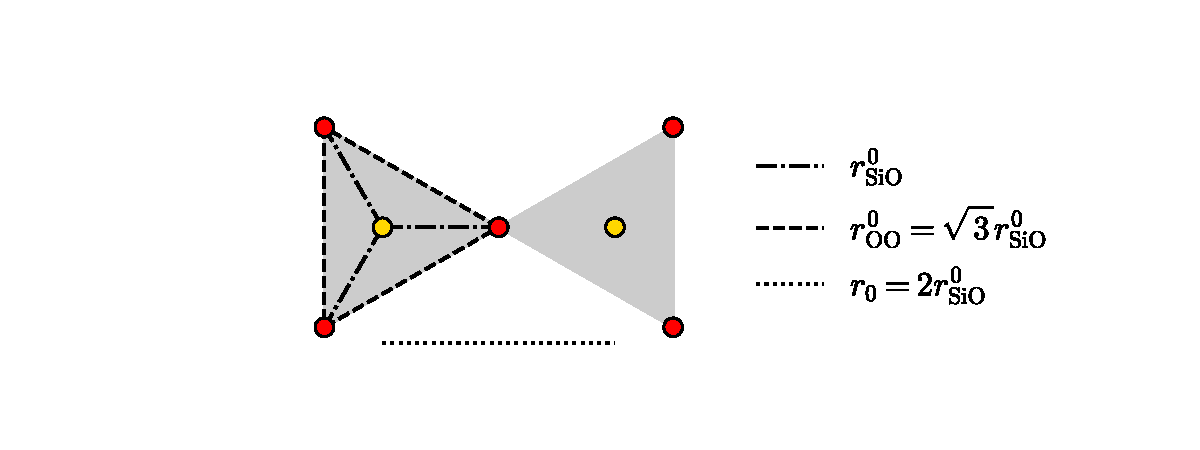
\includegraphics[width=0.6\textwidth]{./figures/bilayers/tr_pot_model.pdf}
 
     \caption{Schematic of the potential model in triangle rafts. Stiff harmonic springs (dashed and dashed\--dotted lines) preserve the triangular subunits, whilst the shifted and cut 24\--12 potential (dotted line) maintains an equilibrium angle of $120^\circ$ between neighbouring subunits.}
     \label{fig:trpotmodel}
\end{figure}

To summarise, the primary aim here is to generate topologies suitable for later investigation using more detailed (and hence more accurate but more
computationally-demanding) potential models. 
As a result, the harmonic springs simply control the local (triangular) geometries whilst the 24-12 potential controls the repulsion between these local polyhedra. 
These functions are chosen as deliberately simple to improve computational efficiency and achieve high throughput of idealised networks. 
Furthermore, the parameters $\fk$ and $\epsilon$ need have no direct physical meaning, simply controlling the
meaning of the system ``temperature'' as discussed below. 
The only requirement is that they generate energies of the same magnitude to allow for efficient
structural evolution.


\subsection{Algorithmic Details}


Using the model detailed above, a Monte Carlo construction algorithm has been developed which allows two\--dimensional networks to be built ring by ring in the shape of a specified function. The main steps of the algorithm are outlined below:
\begin{enumerate}
	\item Take a starting seed, such as a single ring or experimental configuration
	\item Select triangles on which to build the next ring (see figure \ref{fig:triraftalgsearch})
		\label{en:loopstart}
		\begin{enumerate}
			\item Overlay a function on the network (\eg{} circle, square)
			\item Check for atoms with dangling bonds lying inside the function region
			\item If no such atoms exist, systematically increase the function size until an atom is found
			\item Find the next nearest atoms which also have a dangling bonds
			\item Choose the two triangles that correspond to the largest starting ring size	
		\end{enumerate}
	\item Determine the probability of constructing rings of different sizes
		\begin{enumerate}
			\item Build trial rings in the range $k_{\text{min}}$ to $k_{\text{max}}$ (see figure \ref{fig:triraftalgtrial})
			\item Geometry optimise the local structure and calculate minimised potential energy (as explained in section \ref{s:geomopt})
			\item Calculate the probabilities of each ring occurring, $P_k$, equation \eqref{eq:probdist}
		\end{enumerate}
	\item Accept single trial ring according to the probability distribution
		\label{en:loopend}
	\item Repeat steps \ref{en:loopstart} $\rightarrow$ \ref{en:loopend} until the target number of rings is reached
\end{enumerate}
The probability of a ring of size $k$ being accepted, $P_k$, is given by the equation:
\begin{equation}
	\label{eq:probdist}
	P_k=\frac{ \exp{\left[-\left(\mathcal{U}_{k}-\mathcal{U}_k\right)/T\right]}}{\sum\limits_{k}\exp{\left[-\left(\mathcal{U}_{k}-\mathcal{U}_{0}\right)/T\right]}},
\end{equation}
where $\mathcal{U}_k$ and $\mathcal{U}_{0}$ correspond to the energy of the trial structure and lowest energy of all trial structures respectively, and $T$ is a ``temperature''. 
The parameter $T$ controls how easily the potential energy landscape can be explored, and therefore how accessible strained rings become. 
In the low $T$ limit, the acceptance probabilities are dominated by the energy term, and the rings which are selected will be those with the lowest energy. 
Note that this is not necessarily the 6-ring, but rather is dependent on the local environment. On the other hand, in the high $T$ limit, the acceptance probabilities are approximately equal, and rings are selected on a more random basis. 
This is demonstrated in table \ref{tab:prob}, using the example configurations from figure \ref{fig:triraftalgtrial}. 
The ``temperature'' parameter is therefore the primary method for controlling the distribution of ring sizes in constructed networks.

\begin{figure}[bt]
     \centering
     
     \begin{subfigure}[b]{0.45\textwidth}
         \centering
         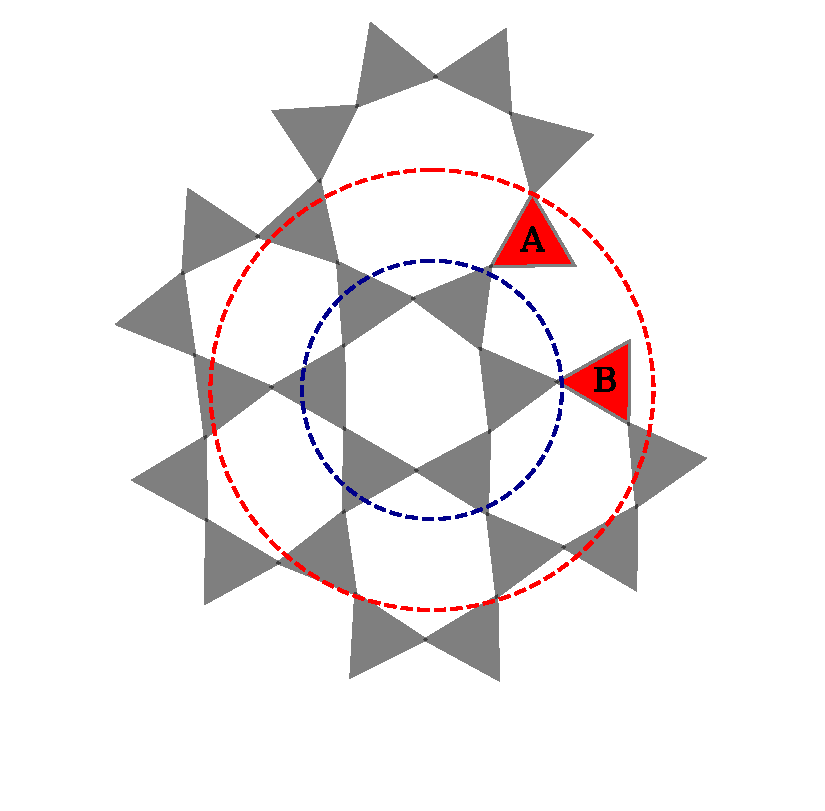
\includegraphics[width=2.5cm]{./figures/bilayers/alg_search_1.pdf}
         \vspace{-1mm}
         \caption{}
         \label{fig:triraftalgsearch1}
     \end{subfigure}
     \hfill
	\begin{subfigure}[b]{0.45\textwidth}
         \centering
         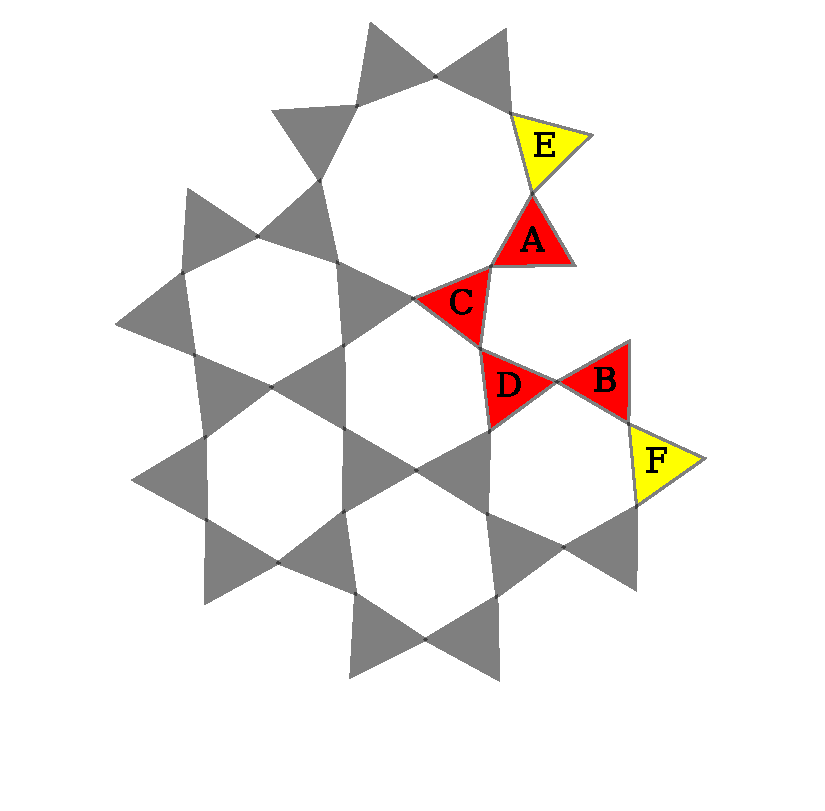
\includegraphics[width=2.5cm]{./figures/bilayers/alg_search_2.pdf}
         \caption{}
         \label{fig:triraftalgsearch2}
     \end{subfigure}
     \hfill
     \caption{Panel (a) shows how triangles used to construct a ring are initially selected. There are no atoms with dangling bonds within the first search region (blue dashed line), and so the search area is extended (red dashed line), where triangles A and B are found. Panel (b) gives the three possibilities for the triangles that will form part of the constructed ring: A–C–D–B, A–E, B–F. As A–C–D–B corresponds to the largest starting ring size this is selected.}
     \label{fig:triraftalgsearch}
     
     \begin{subfigure}[b]{0.18\textwidth}
         \centering
         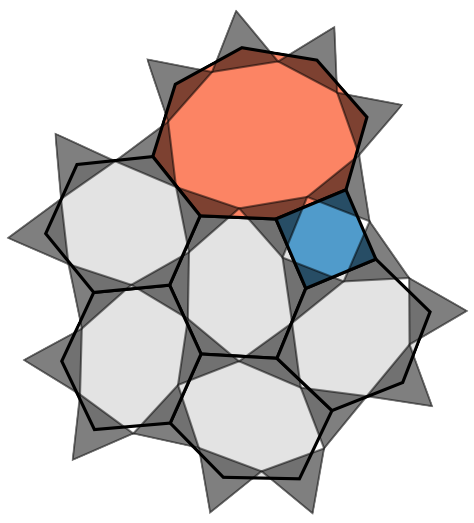
\includegraphics[width=\textwidth]{./figures/bilayers/alg_4.pdf}
         \caption{}
         \label{fig:triraftalgtrial1}
     \end{subfigure}
     \hfill
     \begin{subfigure}[b]{0.18\textwidth}
         \centering
         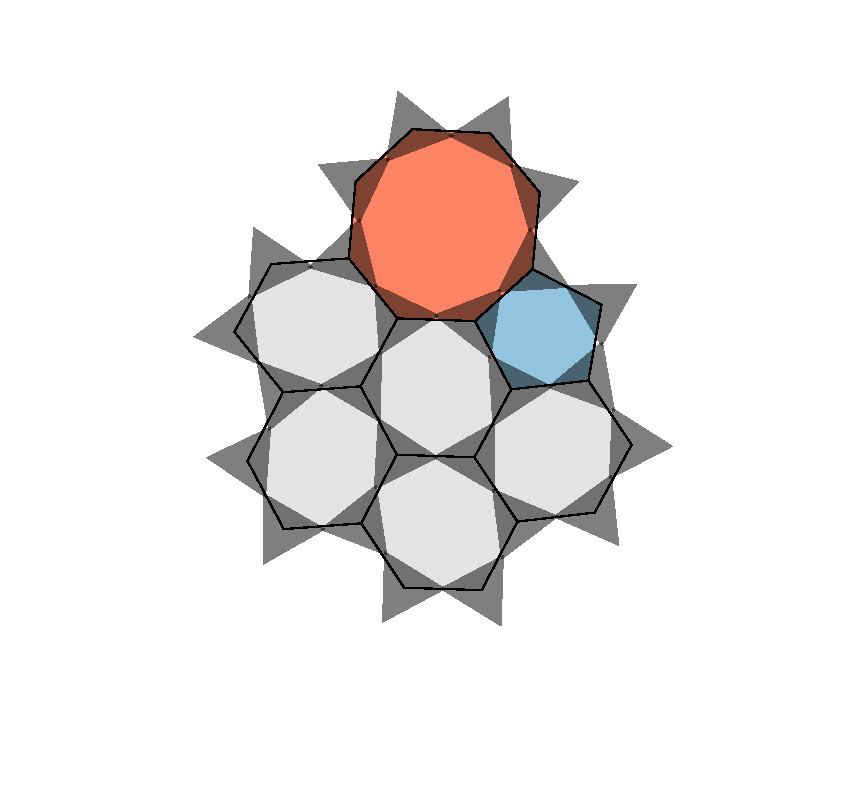
\includegraphics[width=\textwidth]{./figures/bilayers/alg_5.pdf}
         \caption{}
         \label{fig:triraftalgtrial2}
     \end{subfigure}
     \hfill
     \begin{subfigure}[b]{0.18\textwidth}
         \centering
         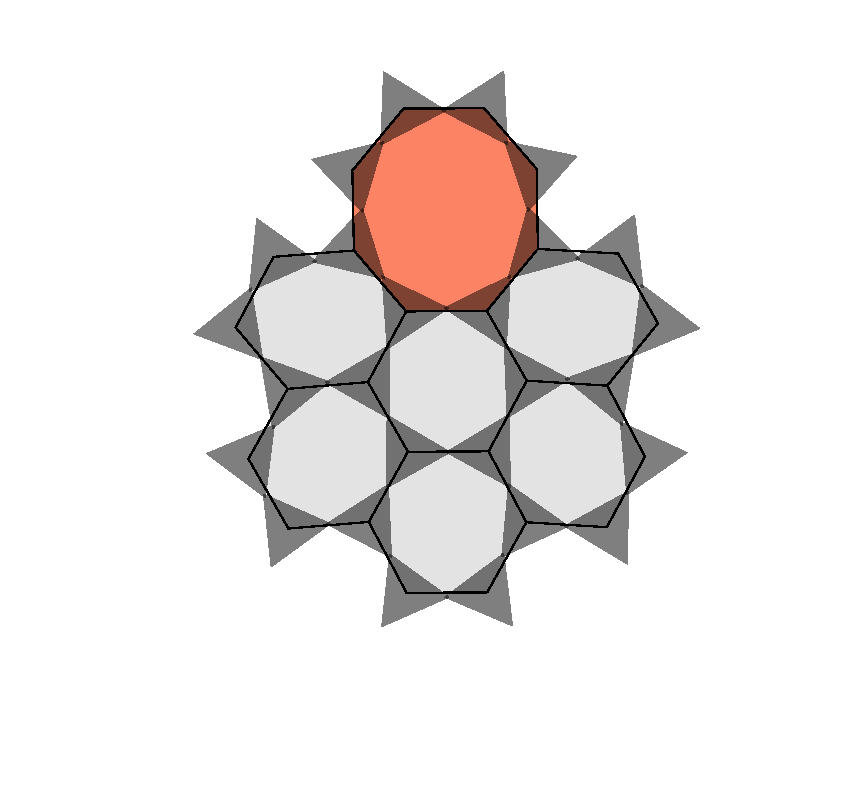
\includegraphics[width=\textwidth]{./figures/bilayers/alg_6.pdf}
         \caption{}
         \label{fig:triraftalgtrial3}
     \end{subfigure}
     \hfill
      \begin{subfigure}[b]{0.18\textwidth}
         \centering
         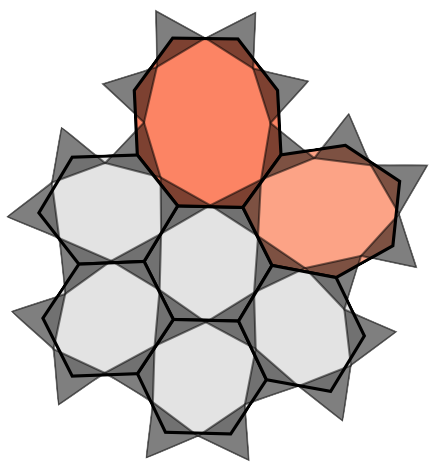
\includegraphics[width=\textwidth]{./figures/bilayers/alg_7.pdf}
         \caption{}
         \label{fig:triraftalgtrial4}
     \end{subfigure}
     \hfill
      \begin{subfigure}[b]{0.18\textwidth}
         \centering
         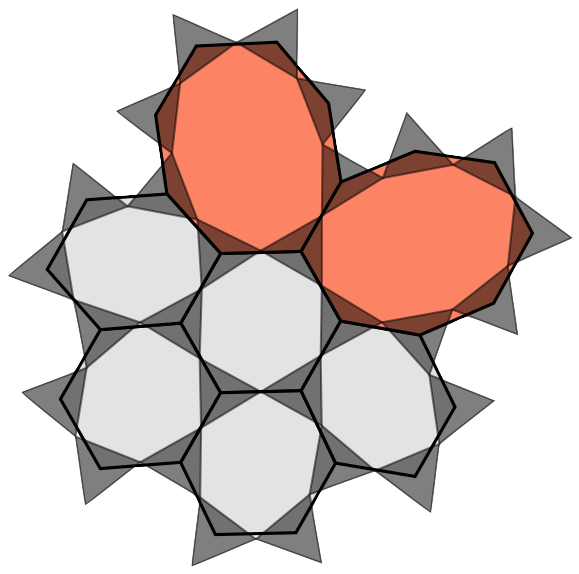
\includegraphics[width=\textwidth]{./figures/bilayers/alg_8.pdf}
         \caption{}
         \label{fig:triraftalgtrial5}
     \end{subfigure}
     \hfill
     \caption{Geometry optimised structures for trial rings in the range $k = 4-8$. The ring structure is shown along with the \sioiii{} triangle}
     \label{fig:triraftalgtrial}
    
\end{figure}

\begin{table}[bt]
	\centering
	\caption{Variation of acceptance probabilities with temperature for the configurations in figure \ref{fig:triraftalgtrial}.}
	\label{tab:prob}
	\begin{tabular}{c c c c c c}
	\toprule
	$P_{k}$ & 4 & 5 & 6 & 7 & 8 \\[0.5mm]
	\midrule
	$T=10^{-4}$ & 0.0000 & 1.0000 & 0.0000 & 0.0000 & 0.0000 \\[0.5mm]
	$T=10^{-3}$ & 0.0000 & 0.8837 & 0.1162 & 0.0001 & 0.0000 \\[0.5mm]
	$T=10^{-2}$ & 0.0336& 0.4104 & 0.3351 & 0.1659 & 0.0550 \\[0.5mm]
	$T=10^{-1}$ & 0.1734 & 0.2227 & 0.2183 & 0.2034 & 0.1822 \\[0.5mm]
	$T=10^{0}\;\;$ & 0.1973 & 0.2023 & 0.2018 & 0.2004 & 0.1982 \\[0.5mm] 
	\bottomrule	
	\end{tabular}
\end{table}

\section{Properties of Triangle Rafts}

The triangle raft method is evaluated in terms of its effectiveness in producing configurations which accurately replicate the network properties of experimental silica bilayers \ie{} the ring statistics and \aw{} parameter.
It is also compared against the existing methods introduced in section \ref{s:triraftexisting}, namely generation from amorphous graphene or molecular dynamics.
This is performed in the wider context of systematically varying the model parameters to explore the behaviour of generic networks of this type.

\subsection{Network Growth}
 
The triangle raft method is robust and controllable, and is able to generate configurations with tuneable ring statistics and topologies.
Results will largely focus on the system where $k=4-10$, denoted $\br{4}{10}$, mimicking the experimentally observed range for silica bilayers. 
Six example configurations are given in figure \ref{fig:triraft}, which are generated with a range of temperatures and growth geometries. 
Figures \ref{fig:triraft1}\--\ref{fig:triraft4} provide a good qualitative analysis of the effect of temperature on the ring structure. 
At low temperature a phase boundary can be seen separating crystalline and amorphous regions, as seen in experimental silica bilayers \cite{Lichtenstein2012b}. 
In these samples although the proportion of small and large rings is low, their positions are highly correlated and chain structures of alternating rings sizes are clearly present. 
These motifs are reminiscent of defects found in a wide range of materials, including amorphous graphene and thin silicon and germanium oxides \cite{Bjorkman2013,Robertson2012,Buchner2017,Lewandowski2018}. 
The increase in temperature is coupled with the emergence of rings of more extreme sizes and regions which could be viewed as nano\--crystalline are dispersed. 
The high temperature limit reveals a fully amorphous structure.

\begin{figure}[h!]
     \centering
     
     \begin{subfigure}[b]{0.35\textwidth}
         \centering
         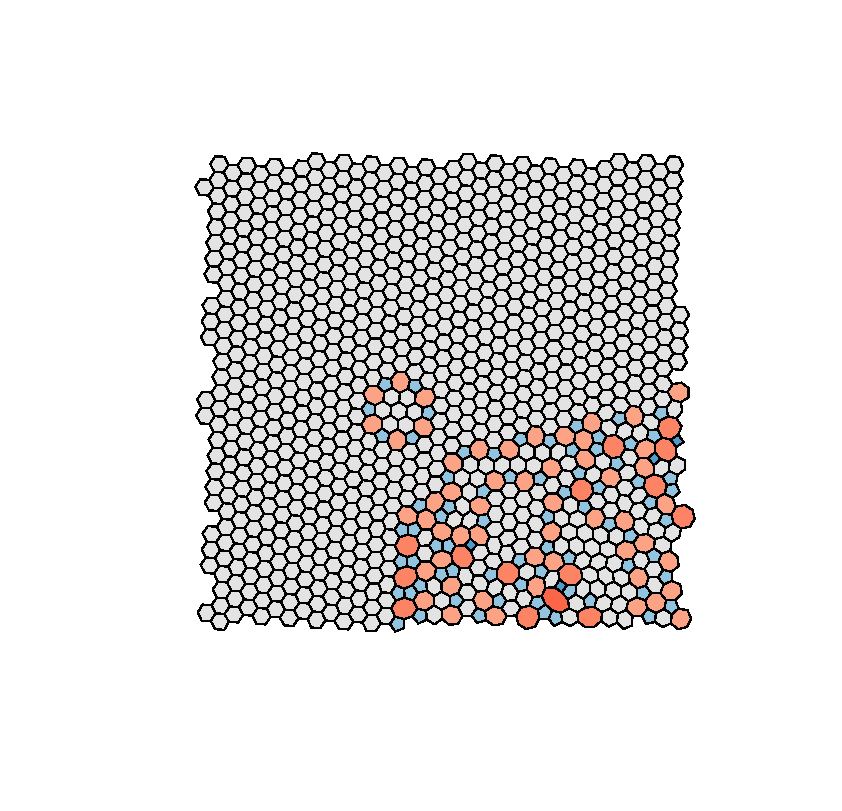
\includegraphics[width=\textwidth]{./figures/bilayers/mx2_sq_1.pdf}
         \caption{}
         \label{fig:triraft1}
     \end{subfigure}
     \hspace{1cm}
     \begin{subfigure}[b]{0.35\textwidth}
         \centering
         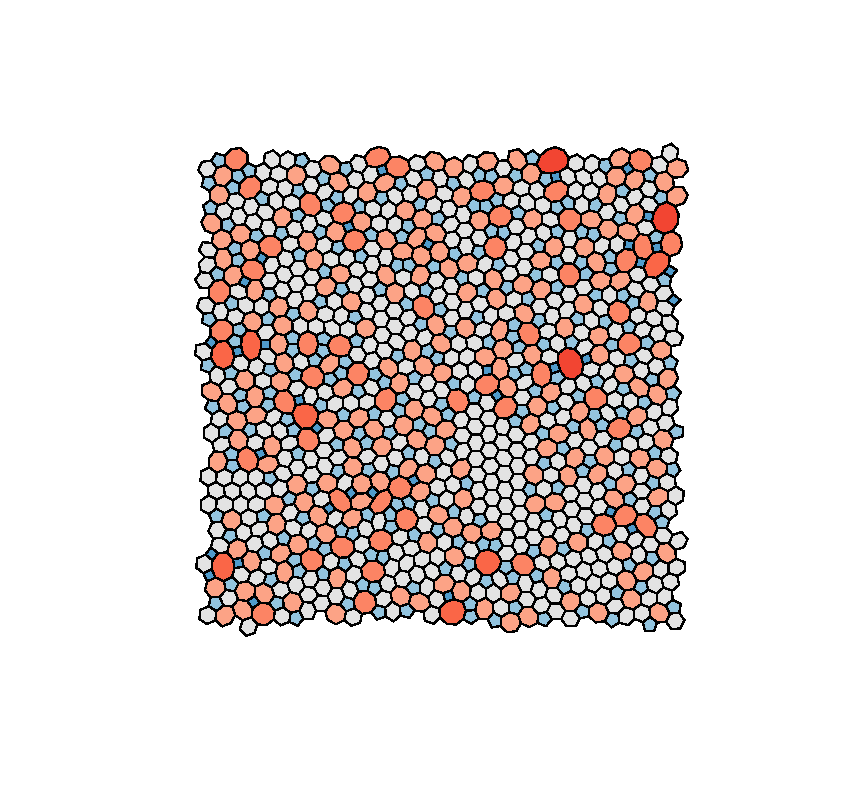
\includegraphics[width=\textwidth]{./figures/bilayers/mx2_sq_2.pdf}
         \caption{}
         \label{fig:triraft2}
     \end{subfigure}
     \hfill
     %\vspace{0.5cm}
     
     \begin{subfigure}[b]{0.35\textwidth}
         \centering
         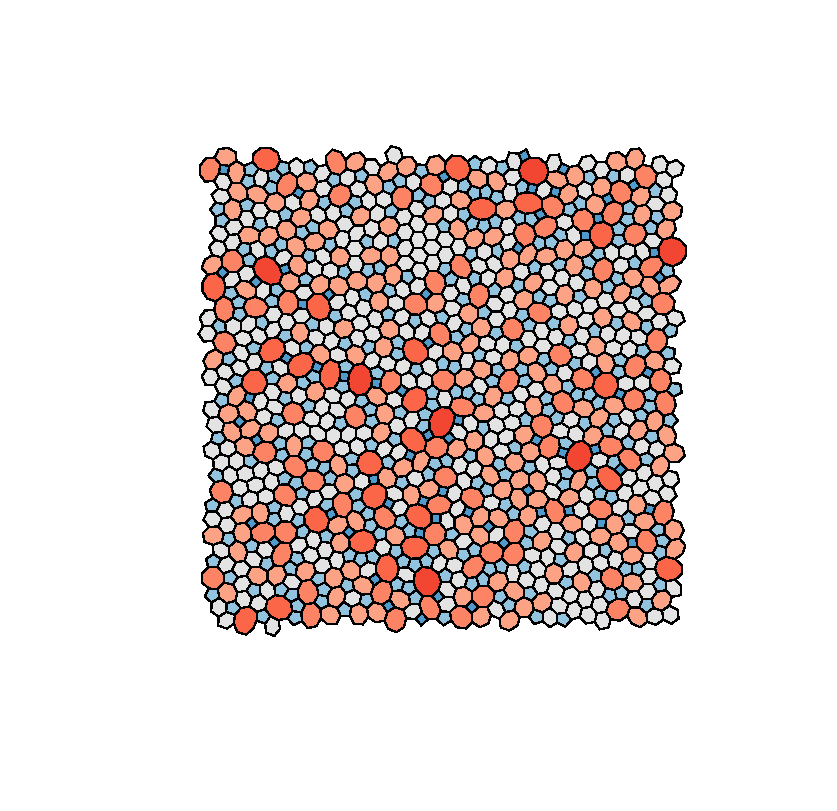
\includegraphics[width=\textwidth]{./figures/bilayers/mx2_sq_3.pdf}
         \caption{}
         \label{fig:triraft3}
     \end{subfigure}
     \hspace{1cm}
      \begin{subfigure}[b]{0.35\textwidth}
         \centering
         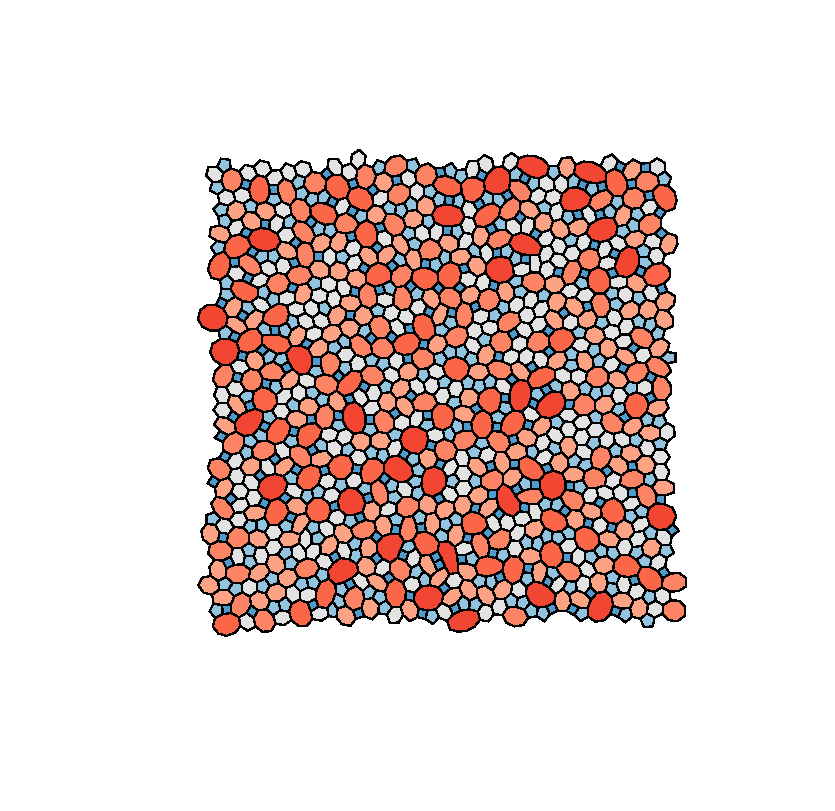
\includegraphics[width=\textwidth]{./figures/bilayers/mx2_sq_4.pdf}
         \caption{}
         \label{fig:triraft4}
     \end{subfigure}
     \hfill
     %\vspace{0.5cm}
     
      \begin{subfigure}[b]{0.35\textwidth}
         \centering
         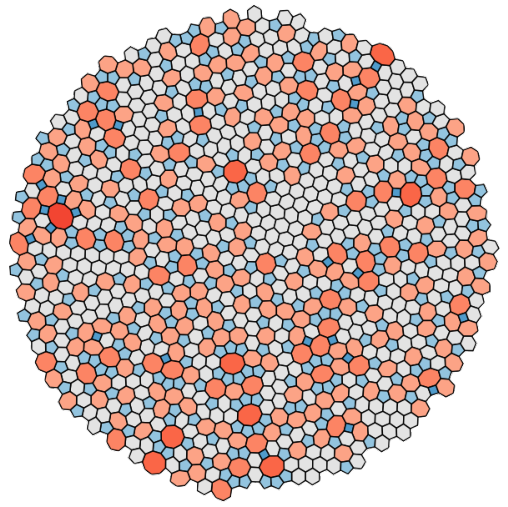
\includegraphics[width=\textwidth]{./figures/bilayers/mx2_circle.pdf}
         \caption{}
         \label{fig:triraft5}
     \end{subfigure}
     \hspace{1cm}
      \begin{subfigure}[b]{0.35\textwidth}
         \centering
         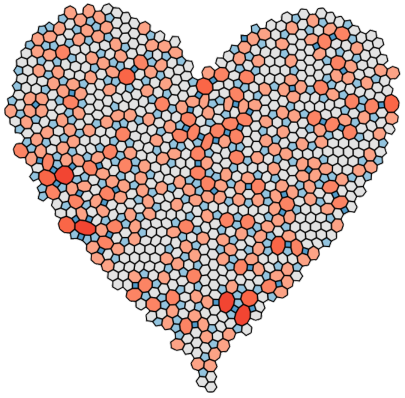
\includegraphics[width=\textwidth]{./figures/bilayers/mx2_heart.pdf}
		\hfill         
         
         \caption{}
         \label{fig:triraft6}
     \end{subfigure}
     
     \caption{Example $1,000$ ring configurations generated with different temperatures and shapes. Panels (a) through (d) show square lattices grown at $T=10^{-4.0},\,10^{-3.0},\,10^{-2.5},\, 10^{-2.0}$ respectively. The samples show the increasing diversity in ring structure as temperature is increased. Panels (e), (f) show configurations with alternative lattice shapes at $T=10^{-3.0}$, demonstrating the flexibility of the method in growing samples with variable geometries. Rings are coloured according to size with $k<6$ as blue, $k=6$ as grey and $k>6$ as red.}
     \label{fig:triraft}
\end{figure}

Figures \ref{fig:triraft5} and \ref{fig:triraft6} give examples of the diverse geometries in which samples may be constructed. 
It is interesting to note that even ``difficult'' shapes, such as those containing concave regions and cusps, do not prevent growth.  
Although the shape does not affect the network topology and is in a sense arbitrary, certain calculations may benefit from the different configurational shapes. 
For instance, molecular dynamics with sliding boundary conditions requires fitting of a smooth function to the sample perimeter, which is facilitated by having a near\--circular form.
Other areas such as percolation problems may benefit from square samples.

\subsection{Network Properties}
\label{s:triraftnetprop}

The quantitative relationship between temperature and ring structure was investigated for three systems of varying ring size ranges;  $\br{5}{7}$, $\br{4}{8}$ and $\br{4}{10}$. 
For each system, 100 samples consisting of 1000 rings were grown at temperatures between $T=10^{-4.5}\rightarrow 10^{-1.5}$. 
The evolution of the combined ring statistics with temperature is presented in figure \ref{fig:trpk}. 
Figures \ref{fig:trpk1}\--\ref{fig:trpk3} give bar representations of the ring size distributions for the three systems, which show different behaviours. 
For $\br{5}{7}$ the individual $p_k$ are all monotonically increasing ($k\neq 6$) or decreasing ($k=6$) functions, but both $\br{4}{8}$ and $\br{4}{10}$ have $p_k$ containing maxima. 
Additionally, both $\br{5}{7}$ and $\br{4}{8}$ achieve uniform distributions in the high temperature limit but $\br{4}{10}$ does not. 

This disparity in behaviour can largely be traced back to the constraint of Euler's theorem. 
As $\br{5}{7}$ comprises of just three ring sizes, Euler's formula demands that $p_5=p_7=\left(1-p_6\right)/2$ and so the system is relatively well defined. 
Hence, as the 5 and 7-rings are more strained than the 6-ring, $p_5$ and $p_7$ show a systematic increase with temperature. 
Furthermore, the uniform equilibrium distribution can only satisfy Euler's formula when the ring size range is symmetric about 6, as is observed for $\br{5}{7}$ and $\br{4}{8}$. 
The form of the ring statistics at intermediate temperatures and for $\br{4}{10}$ follow the maximum entropy solutions according to \lm's law, discussed in section \ref{s:lemaitre} and later in this section.

\begin{figure}[bt]
     \centering
     
     \begin{subfigure}[b]{0.45\textwidth}
         \centering
         \includegraphics[width=\textwidth]{./figures/bilayers/triraft_57.pdf}
         \caption{$\br{5}{7}$}
         \label{fig:trpk1}
     \end{subfigure}
     \hfill
	\begin{subfigure}[b]{0.45\textwidth}
         \centering
         \includegraphics[width=\textwidth]{./figures/bilayers/triraft_48.pdf}
         \caption{$\br{4}{8}$}
         \label{fig:trpk2}
     \end{subfigure}
     \hfill
     
	\vspace{0.5cm}          
     \begin{subfigure}[b]{0.45\textwidth}
         \centering
         \includegraphics[width=\textwidth]{./figures/bilayers/triraft_410.pdf}
         \caption{$\br{4}{10}$}
         \label{fig:trpk3}
     \end{subfigure}
     \hfill
	\begin{subfigure}[b]{0.45\textwidth}
         \centering
         \includegraphics[width=\textwidth]{./figures/bilayers/triraft_line_410.pdf}
         \caption{$\br{4}{10}$}
         \label{fig:trpk4}
     \end{subfigure}
     \hfill
   
     \caption{Variation in ring statistics with temperature over a given allowable $k$\--range. Panels (a)-(c) show bar graph representations of the ring statistics, coloured by temperature, for the $\br{5}{7}$, $\br{4}{8}$ and $\br{4}{10}$ systems, respectively. Panel (d) gives an alternative line graph representation of the ring statistics for $\br{4}{10}$, coloured by ring size, along with the Aboav\--Weaire parameter. The temperature which gives the best match to the experimentally observed amorphous region is also highlighted (vertical black dashed line).}
     \label{fig:trpk}
\end{figure}

The ring distribution for $\br{4}{10}$ is also shown as a function of temperature in figure \ref{fig:trpk4}, along with the value of the \aw{} parameter, $\alpha$, allowing for more facile comparison with experiment. 
The temperature which gives the best agreement between our model and amorphous experimental samples is highlighted by the vertical dashed line. 
The values of $p_k$ and $\alpha$ are provided in table \ref{tab:trpk}, alongside results from two experimental samples. 
It is evident that the model can be successfully tuned to match the topology of the experimental system. 
Not only are the ring distributions in very good accordance, but also the ring correlations, which have until now proved difficult to capture. 
This provides confidence that this simplified but physically motivated triangle raft model is able to reproduce the behaviour of real systems.

\begin{landscape}
\begin{table}
\centering
\caption{Comparison of silica bilayer samples from experiment, computational modelling and theory.}
\label{tab:trpk}
\begin{threeparttable}
\begin{tabular}{@{}ccccccccccc@{}}
\toprule
& \multicolumn{2}{c}{Experiment} & \phantom{xxx} & \multicolumn{4}{c}{Computation} & \phantom{xxx} & \multicolumn{1}{c}{Theory} \\ 
\cmidrule{2-3} \cmidrule{5-8} \cmidrule{10-10}
& Ru(0001) \cite{Buchner2016a} & Graphene \cite{Huang2012} & & MC\tnote{a}\, \cite{Kumar2014} & MC\tnote{a}\, \cite{Kumar2014} & MD\tnote{b}\, \cite{Roy2018} & TR\tnote{c} & & \lm{} \cite{Gervois1992}  \\ 
\midrule
$N$ & 317    & 444    &&    216 & 418      & $16 \times 85000$ & $1000 \times 100$ && \--- \\ 
$p_3$  &0.0000 & 0.0000 && 0.00 & 0.00     & 0.0038            & 0.0000 && 0.0000 \\ 
$p_4$  &0.0379 & 0.0383 && 0.02   & 0.00     & 0.0537            & 0.0295 && 0.0280 \\  
$p_5$  &0.2744 & 0.2725 && 0.33   & 0.37     & 0.2686            & 0.2786 && 0.2834 \\
$p_6$  &0.4448 & 0.4189 && 0.37   & 0.32     & 0.3773            & 0.4234 &&  0.4200 \\  
$p_7$  &0.1609 & 0.2117 && 0.21   & 0.25     & 0.2224            & 0.2034 && 0.2077 \\  
$p_8$  &0.0757 & 0.0495 && 0.07   & 0.06     & 0.0602            & 0.0544 && 0.0518 \\ 
$p_9$  &0.0063 & 0.0068 && <0.01  & 0.00     & 0.0118            & 0.0097 && 0.0082 \\
$p_{10}$  &0.0000 & 0.0023 && 0.00 & 0.00  & 0.0018            & 0.0010 && 0.0009 \\
$p_{>10}$  &0.0000 & 0.0000 && 0.00 & 0.00 & 0.0004            & 0.0000 && 0.0000 \\ 
$\mu_2$ &  0.9460 & 0.9333 &&  0.94 & 0.86 & 1.1302 & 0.9208 && 0.8985 \\ 
$\alpha$  &0.32   & 0.33 && 0.18 & 0.23 & 0.25 & 0.32 && \--- \\
\bottomrule
\end{tabular}
\begin{tablenotes}
  Note: Each method is given alongside the number of rings in the sample, $N$, followed by the ring statistics, $p_k$, the second moment of the ring statistics, $\mu_2$, and the \aw{} parameter, $\alpha$ \\
  \item[a] Bond switching \mc{} (graphene potential)
  \item[b] Molecular dynamics
  \item[c] Triangle rafts, this work, $T=10^{-3}$
\end{tablenotes}
\end{threeparttable}
\end{table}
\end{landscape}

Table \ref{tab:trpk} also lists the ring statistics obtained from previous computational studies which used both Monte Carlo and molecular dynamics methods. 
As mentioned in the review of these methods above, neither fully succeeds in accurately capturing the topology of silica bilayers.
Kumar \etal{} attempted to transform an amorphous graphene structure generated from bond switching \mc{} into a silica bilayer.
The ring statistics of the resulting structure were approximately correct, but the proportion of 5\-- and 6\-- rings over\-- and under\--estimated respectively.
In addition the \aw{} parameter was substantially lower than experiment, indicating a relative lack of structure in the ring ordering.
The origin of these discrepancies is likely the use of a graphene potential model.
The increased stiffness of the carbon network (which unlike silica lacks bridging oxygens) means a high temperature must be used to obtain an amorphous structure with the required disorder.
This leads to heavily distorted rings (as noted in the original paper) which reduces the requirement for small rings to be adjacent to large.

Roy \etal{} have an alternative approach of generating configurations with an effective pair potential and molecular dynamics.
As can be seen the ring statistics are closer to the experimental values, but now contain artefacts, with a significant fraction of highly strained 3\--membered rings and large rings up to $k=14$.
These manifest as a result of the artificially high cooling rates in the computational studies which trap defect states in the configurations. 
Once again the final \aw{} parameter, $\alpha$, is underestimated.

It is worth re\--emphasising here that the triangle raft method is able to replicate experimental values of both $p_k$ and $\alpha$, due to its tuneable approach and ``organic'' growth mechanism, where sample formation is not influenced by enforced periodicity. 
Beyond this, the controllable nature of the method also allows insight into key questions about silica bilayers, for instance the form of the ring distribution in this amorphous phase. 
As detailed in section \ref{s:lemaitre}, the maximum entropy ring distribution can be calculated numerically given the value of $p_6$.
For example, table \ref{tab:trpk} gives the maximum entropy solution for $p_6=0.42$, which agrees very well with the results from triangle rafts and experiment.
This second moment of the distribution, $\mu_2$, is then uniquely related to $p_6$ via \lm's law, shown as the black line in in figure \ref{fig:trlm1}.


\begin{figure}[bt]
     \centering
     
     \begin{subfigure}[b]{0.45\textwidth}
         \centering
         \includegraphics[width=\textwidth]{./figures/bilayers/tri_raft_lm_1.pdf}
         \caption{}
         \label{fig:trlm1}
     \end{subfigure}
     \hfill
     \begin{subfigure}[b]{0.45\textwidth}
         \centering
         \includegraphics[width=\textwidth]{./figures/bilayers/tri_raft_lm_3.pdf}
         \caption{}
         \label{fig:trlm2}
     \end{subfigure}
     \hfill
     \begin{subfigure}[b]{0.45\textwidth}
         \centering
         \includegraphics[width=\textwidth]{./figures/bilayers/tri_raft_lm_2.pdf}
         \caption{}
         \label{fig:trlm3}
     \end{subfigure}
     \hfill

     \caption{Evolution of ring statistics (a), entropy (b) and potential energy (c) of triangle rafts with temperature. The experimental value of $p_6\approx 0.4$ occurs just before the exponential increase in potential energy, reflecting the balance of energetic and entropic factors.}
     \label{fig:trlm}
\end{figure}


However, \lm's law gives no information on why a particular maximum entropy distribution is found for a given system.
The triangle raft method allows systematic generation of configurations with different $p_6$ values by tuning the temperature parameter. 
The resulting configurations follow \lm's law across the entire temperature range. 
Figures \ref{fig:trlm} gives the results from the individual 1000 ring samples, coloured by temperature.
Figures \ref{fig:trlm1} and \ref{fig:trlm2} compare the observed $\mu_2$ and $\mathcal{S}$ (entropy) of the generated configurations to those expected from \lm's law, showing the law provides a good fit, with only a small deviation observed for $p_k>0.5$. 

Figure \ref{fig:trlm3} plots the geometry optimised potential energy of the samples against $p_6$, which increases as the ring sizes become more diverse. 
The curve is split into two regimes, with gradual increase in energy from $p_6=1.0\rightarrow 0.4$ followed by exponential increase for $p_6<0.4$. 
This is consistent with the information in figure \ref{fig:trpk4} which shows that below $p_6\approx 0.4$, not only does the number of extreme ring sizes increase rapidly, but they become less correlated with a lower $\alpha$, decreasing the number of favourable small\--large ring pairings.

It can now be proposed why the experimental amorphous distributions are found with a value of $p_6\approx 0.4$. 
The system aims to maximise entropy by obtaining a ring distribution along the \lm{} curve with the minimum $p_6$ possible. 
However, for $p_6<0.4$ the energetic cost becomes prohibitively large, as higher entropy distributions can only be achieved by increasing the proportion of extreme ring sizes at the expense of relatively low strain 5- and 7- rings.
Interestingly it is also evident why no configurations are present below $p_6\approx 0.16$, even at the highest temperature.
Below this point, the entropy of the $\br{4}{10}$ system decreases whilst the energy continues to rise and so there is no driving force to sample this area of phase space.

\subsection{Physical Properties}
\label{s:trphysprop}

As an additional check that the developed triangle raft model behaves physically, 
the angle distribution between adjacent \sioiii{} units, $f\left(\theta\right)$, was calculated for the $\br{4}{10}$ system across the range of temperatures studied. 
The results are summarised in figure \ref{fig:trang}. 
The angle distributions are necessarily symmetric about $120^\circ$, as each triangle pair contributes two complementary angles. 
At lower temperatures the distribution is dominated by angles close to $120^\circ$, as a consequence of the large proportion of near strainless six membered rings.
Furthermore, at the temperature corresponding to the amorphous experimental region, $T=10^{-3}$, the distribution has a similar extent to the angle distribution found in experimental samples (see for example figure 7 reference \cite{Roy2018}). 
However, as the temperature increases, the form of $f\left(\theta\right)$ does not simply broaden as might be expected, but becomes bimodal. 
This can be rationalised by considering the angles that would be present in regular polygons of different sizes, marked by vertical lines in figure \ref{fig:trang}.  These ideal angles are clustered away from the mean value of $120^\circ$, and hence increasing the diversity of ring sizes through temperature acts to shift the most commonly observed angles from the central value of $120^\circ$. 
It is therefore interesting to note that increasing structure in the angle distribution does not necessarily translate to increased order in the atomic configurations.

\begin{figure}[bt]
     \centering
     
     \begin{subfigure}[b]{0.45\textwidth}
         \centering
         \includegraphics[width=\textwidth]{./figures/bilayers/tri_raft_angle.pdf}
         \caption{}
         \label{fig:trang}
     \end{subfigure}
     \hfill
     
     \begin{subfigure}[b]{0.45\textwidth}
         \centering
         \includegraphics[width=\textwidth]{./figures/bilayers/tri_raft_area.pdf}
         \caption{}
         \label{fig:trarea}
     \end{subfigure}
     \hfill
     \begin{subfigure}[b]{0.45\textwidth}
         \centering
         \includegraphics[width=\textwidth]{./figures/bilayers/ellipse_area.pdf}
         \caption{}
         \label{fig:trellipse}
     \end{subfigure}
     \hfill

     \caption{Panel (a) gives the ring angle distribution function for triangle rafts formed at different temperatures. Panel (b) compares the regularity of rings in computational and experimental amorphous configurations, with points indicating the mean value and bars corresponding to the standard deviation. Experimental data is taken from ref. \cite{Kumar2014}. Panel (c) shows the effect on the area when distorting a circle to an ellipse whilst maintaining a constant perimeter length.}
     \label{fig:trangarea}
\end{figure}

A final check comes from examining the ring areas in the generated configurations.
Inspection of amorphous experimental samples reveals that the rings appear highly regular in shape. 
This can be quantified by determining the average dimensionless area for each ring size, $A_k$, and comparing it to the area of the corresponding regular polygon, $A_k^0$, where:
\begin{align}
	A_k &= \frac{\langle Area\left(k\right) \rangle}{\left(r_{\text{SiSi}}^{0}\right)^2}, \label{eq:trarea} \\[0.5em]
	A_k^0 &= \frac{k}{4\tan\left(\pi / k \right)} \label{eq:trarea0}.
\end{align}
As the regular polygon has the maximum achievable area for a given ring size, the ratio $A_k / A_k^0$ is expected to lie in the range $0\rightarrow 1$, with a lower value corresponding to increased deviation from regularity, and assuming $r_{\text{SiSi}}^{0}$ to be fixed.

The study by Kumar \etal{} found that whereas for experimental configurations, $A_k / A_k^0 \approx 1$, configurations generated using thier bond switching method generally displayed ratios much less than unity \cite{Kumar2012}, indicative of large distortions in the ring structure. 
For larger rings, a value of $A_k / A_k^0 > 1$ was also found, which can only be achieved if there is appreciable bond stretching (see equations \eqref{eq:trarea}, \eqref{eq:trarea0}). 

The analogous results for the method presented in this chapter can be found in figure \ref{fig:trarea}, for $T=10^{-3}$. 
This figure demonstrates that there is now good agreement between experimental and computational results. 
In both cases the deviation from regularity increases with ring size, as the flexibility of the rings increases. 
Again it can be proposed that the difference between current and previous methods could be due to the lack of enforced periodicity on the system. 
By allowing the network to grow relatively freely, the system can avoid a build up of strain associated with maintaining periodic boundaries.

Even with this analysis, an argument can be made that by visual inspection the rings in the experimental configurations are still more regular than those generated from computational samples. 
Therefore one can consider if deformation of a ring should be expected to lead to significant reduction in area. 
This can be explored by considering the distortion of a circle to an ellipse. 
The degree of distortion can be described by the eccentricity of the ellipse,
\begin{equation}
	\xi = \left(1-\frac{b^2}{a^2}\right)^{1/2},
\end{equation}
where $a$, $b$ are the major and minor axis radii respectively. 
This change in area with distortion is shown in figure \ref{fig:trellipse}, the calculation of which can be found in appendix \ref{app:derivellipse}. 
As can be seen, a large degree of eccentricity is needed for a significant change in the observable area. 
For example, if $a=1.5 b$, the area is still $\approx0.94\%$ of the area of the corresponding circle. 

For silica networks the Si\---Si distances lie in a narrow range because of the covalent nature of the atomic bonding and the near-linear Si-O-Si bridges
which join the two layers. 
Hence we would expect similar behaviour to occur, with ring areas relatively invariant to distortions in the ring shape (this same analysis would not be expected to hold for foams for example, where the length of the boundary is much more flexible). 
This suggests that the ring area is not the most suitable metric for quantifying the regularity of rings in systems such as this, and could explain any disagreement between the seemingly near ideal ring areas and the visual evidence. 
As previously stated, although the potential model used is physically motivated, it is lightweight in order to facilitate generation of a large number of configurations with the correct network topology. 
In future it would be informative to see if the required regularity can be achieved by geometry optimising the resulting bilayer configurations with a more accurate potential, such as the TS potential which includes potentially significant electrostatic interactions including many-body polarisation effects \cite{Tangney2002}.

\section{Chapter Conclusions}

A method has been developed for effective modelling of silica bilayers and related materials.
Bilayers are represented as triangle rafts, which are sequentially constructed from a seed using a stochastic growth algorithm.
The algorithm is flexible, allowing control over the ring size distribution and overall system topology.
The success of triangle rafts in modelling silica bilayers has been demonstrated by the values of the \aw{} parameter, $\alpha$, which are are more commensurate with those obtained from experimental imaging than configurations generated by previous methods.
Moreover, consideration of the ring areas shows that triangle raft configurations contain highly regular polygons - another experimental observation that has proved challenging to previously capture.

The real advantage of the method is that it enables a computationally tractable and systematic exploration of bilayer systems at increasing levels of disorder.
This has been employed in this chapter for a detailed analysis of \lm's
law, which rationalised why the fraction of six-membered rings observed
in real systems is often $\approx$0.4. 
However, it will also be used in chapter \ref{ch:ph} to investigate the use of persistent homology in amorphous materials.
The ability to build a triangle raft from any user\--defined starting seed also opens further possibilities for the method.
In particular, it would be interesting to see how network growth is affected by the presence of a template, which could be for example a very large ring.
This could lead to insight into how to control pore geometries in these materials.








%% APPENDICES %% 
% Starts lettered appendices, adds a heading in table of contents, and adds a
%    page that just says "Appendices" to signal the end of your main text.
%\startappendices
% Add or remove any appendices you'd like here:
%\begin{savequote}[8cm]
\textlatin{Cor animalium, fundamentum e\longs t vitæ, princeps omnium, Microco\longs mi Sol, a quo omnis vegetatio dependet, vigor omnis \& robur emanat.}

The heart of animals is the foundation of their life, the sovereign of everything within them, the sun of their microcosm, that upon which all growth depends, from which all power proceeds.
  \qauthor{--- William Harvey \cite{harvey_exercitatio_1628}}
\end{savequote}

\chapter{\label{app:1-cardiophys}Review of Cardiac Physiology and Electrophysiology}

\minitoc

Appendices are just like chapters.  Their sections and subsections get numbered and included in the table of contents; figures and equations and tables added up, etc.  Lorem ipsum dolor sit amet, consectetur adipiscing elit. Sed et dui sem. Aliquam dictum et ante ut semper. Donec sollicitudin sed quam at aliquet. Sed maximus diam elementum justo auctor, eget volutpat elit eleifend. Curabitur hendrerit ligula in erat feugiat, at rutrum risus suscipit. Pellentesque habitant morbi tristique senectus et netus et malesuada fames ac turpis egestas. Integer risus nulla, facilisis eget lacinia a, pretium mattis metus. Vestibulum aliquam varius ligula nec consectetur. Maecenas ac ipsum odio. Cras ac elit consequat, eleifend ipsum sodales, euismod nunc. Nam vitae tempor enim, sit amet eleifend nisi. Etiam at erat vel neque consequat.

\section{Anatomy}
\label{sec:anatomy}

Lorem ipsum dolor sit amet, consectetur adipiscing elit. Donec accumsan cursus neque. Pellentesque eget tempor turpis, quis malesuada dui. Proin egestas, sapien sit amet feugiat vulputate, nunc nibh mollis nunc, nec auctor turpis purus sed metus. Aenean consequat leo congue volutpat euismod. Vestibulum et vulputate nisl, at ultrices ligula. Cras pulvinar lacinia ipsum at bibendum. In ac augue ut ante mollis molestie in a arcu.

Etiam vitae quam sollicitudin, luctus tortor eu, efficitur nunc. Vestibulum maximus, ante quis consequat sagittis, augue velit luctus odio, in scelerisque arcu magna id diam. Proin et mauris congue magna auctor pretium id sit amet felis. Maecenas sit amet lorem ipsum. Proin a risus diam. Integer tempus eget est condimentum faucibus. Suspendisse sem metus, consequat vel ante eget, porttitor maximus dui. Nunc dapibus tincidunt enim, non aliquam diam vehicula sed. Proin vel felis ut quam porta tempor. Vestibulum elit mi, dictum eget augue non, volutpat imperdiet eros. Praesent ac egestas neque, et vehicula felis.

Pellentesque malesuada volutpat justo, id eleifend leo pharetra at. Pellentesque feugiat rutrum lobortis. Curabitur hendrerit erat porta massa tincidunt rutrum. Donec tincidunt facilisis luctus. Aliquam dapibus sodales consectetur. Suspendisse lacinia, ipsum sit amet elementum fermentum, nulla urna mattis erat, eu porta metus ipsum vel purus. Fusce eget sem nisl. Pellentesque dapibus, urna vitae tristique aliquam, purus leo gravida nunc, id faucibus ipsum magna aliquet ligula. Lorem ipsum dolor sit amet, consectetur adipiscing elit. Proin sem lacus, rutrum eget efficitur sed, aliquam vel augue. Aliquam ut eros vitae sem cursus ultrices ut ornare urna. Nullam tempor porta enim, in pellentesque arcu commodo quis. Interdum et malesuada fames ac ante ipsum primis in faucibus. Curabitur maximus orci purus, ut molestie turpis pellentesque ut.

Donec lacinia tristique ultricies. Proin dignissim risus ut dolor pulvinar mollis. Proin ac turpis vitae nibh finibus ullamcorper viverra quis felis. Mauris pellentesque neque diam, id feugiat diam vestibulum vitae. In suscipit dui eu libero ultrices, et sagittis nunc blandit. Aliquam at aliquet ex. Nullam molestie pulvinar ex vitae interdum. Praesent purus nunc, gravida id est consectetur, convallis elementum nulla. Praesent ex dolor, maximus eu facilisis at, viverra eget nulla. Donec ullamcorper ante nisi. Sed volutpat diam eros. Nullam egestas neque non tortor aliquet, sed pretium velit tincidunt. Aenean condimentum, est ac vestibulum mattis, quam augue congue augue, mattis ultrices nibh libero non ante. Lorem ipsum dolor sit amet, consectetur adipiscing elit.

Aenean volutpat eros tortor, non convallis sapien blandit et. Maecenas faucibus nulla a magna posuere commodo. Nullam laoreet ante a turpis laoreet malesuada. Phasellus in varius sem. Vestibulum sagittis nibh sed tincidunt blandit. Donec aliquam accumsan odio sit amet lacinia. Integer in tellus diam. Vivamus varius massa leo, vitae ullamcorper metus pulvinar sed. Maecenas nec lorem ornare, elementum est quis, gravida massa. Suspendisse volutpat odio ex, ac ultrices leo ultrices vel. Sed sed convallis ipsum. Pellentesque euismod a nulla sed rhoncus. Sed vehicula urna vitae mi aliquet, non sodales lacus ullamcorper. Duis mattis justo turpis, id tempus est tempus eu. Curabitur vitae hendrerit ligula.

Curabitur non pretium enim, in commodo ligula. Etiam commodo eget ligula a lacinia. Vestibulum laoreet ante tellus, vel congue sapien ornare in. Donec venenatis cursus velit vitae pulvinar. Pellentesque habitant morbi tristique senectus et netus et malesuada fames ac turpis egestas. Suspendisse in metus lectus. Pellentesque gravida dolor eget finibus imperdiet. Duis id molestie tortor. Mauris laoreet faucibus facilisis. Aliquam vitae dictum massa, sit amet dignissim lacus.

Fusce eleifend tellus id ex consequat maximus. Donec ultrices ex ut turpis ornare, non molestie mi placerat. Nulla sit amet auctor nunc, sit amet euismod elit. Phasellus risus tellus, condimentum a metus et, venenatis tristique urna. Cras mattis felis eget ipsum fermentum egestas. Ut augue odio, venenatis id convallis vel, congue quis augue. Maecenas sed maximus est, posuere aliquet tortor. Ut condimentum egestas nisi eu porttitor. Ut mi turpis, posuere id lorem vel, elementum tempor arcu.

Morbi nisl arcu, venenatis non metus ac, ullamcorper scelerisque justo. Nulla et accumsan lorem. Mauris aliquet dui sit amet libero aliquet, in ornare metus porttitor. Integer ultricies urna eu consequat ultrices. Maecenas a justo id purus ultricies posuere sed et quam. Cum sociis natoque penatibus et magnis dis parturient montes, nascetur ridiculus mus. Sed eleifend risus quis aliquet gravida. Nullam ac erat porta est bibendum dictum in a dolor. Nam eget turpis viverra, vulputate lectus eget, mattis ligula. Nam at tellus eget dui lobortis sodales et ut augue. In vestibulum diam eget mi cursus, ut tincidunt nulla pellentesque.

Aliquam erat volutpat. Sed ultrices massa id ex mattis bibendum. Nunc augue magna, ornare at aliquet gravida, vehicula sed lorem. Quisque lobortis ipsum eu posuere eleifend. Duis bibendum cursus viverra. Nam venenatis elit leo, vitae feugiat quam aliquet sed. Cras velit est, tempus ac lorem sed, pharetra lobortis ipsum. Donec suscipit gravida interdum. Nunc non finibus est. Nullam turpis elit, tempus non ante.

\section{Mechanical Cycle}

Lorem ipsum dolor sit amet, consectetur adipiscing elit. Aenean tellus est, suscipit sed facilisis quis, malesuada at ipsum. Nam tristique urna quis quam iaculis, et mattis orci pretium. Praesent euismod elit vel metus commodo ultrices. Vestibulum et tincidunt ex, in molestie ex. Donec ullamcorper sollicitudin accumsan. Etiam ac leo turpis. Duis a tortor felis. Nullam sollicitudin eu purus ac hendrerit. Nam hendrerit ligula libero, eget finibus orci bibendum a. Aenean ut ipsum magna.

Ut viverra, sapien sed accumsan blandit, nisi sem tempus tellus, at suscipit magna erat ornare nunc. Proin lacinia, nisi ut rutrum malesuada, nibh quam pellentesque nunc, sit amet consectetur purus felis ac tortor. Suspendisse lacinia ipsum eu sapien pellentesque mattis. Mauris ipsum nunc, placerat non diam vel, efficitur laoreet nunc. Sed lobortis, ipsum eget gravida facilisis, sem nulla viverra mi, in placerat eros sem viverra lacus. Aliquam porta aliquet diam vel commodo. Nulla facilisi. Duis erat libero, lobortis vel hendrerit vitae, sagittis id dui. Nulla pretium eros nec quam tincidunt, vel luctus mi aliquam. Integer imperdiet purus in est tristique venenatis. Ut pellentesque, nunc vitae iaculis ultricies, urna turpis dignissim risus, a laoreet felis magna nec erat.

Quisque sollicitudin faucibus ligula, et egestas nibh dictum sit amet. Proin eu mi a lectus congue pretium eu quis arcu. Suspendisse vehicula libero eu ipsum aliquam, vel elementum nibh mattis. Sed sed sapien vitae turpis tristique pulvinar a ut metus. Etiam semper gravida est, mollis gravida est porta ac. Proin eget tincidunt erat. Maecenas ultrices erat eget purus ultricies, ut lacinia arcu dictum. Nam et nisi sit amet ex congue mattis vel eget lorem. Aliquam erat volutpat. Pellentesque porttitor nibh vitae elementum consectetur. Aenean et est lobortis, congue sapien non, ullamcorper sapien. Ut facilisis sem non dapibus vehicula.

Mauris euismod odio dolor, sit amet gravida mauris placerat et. Curabitur nec dolor non nibh molestie lobortis dignissim non ante. Nullam rutrum lobortis ultrices. Aenean ex erat, elementum sed maximus id, posuere id quam. Proin rutrum ex elit, pretium aliquam risus finibus at. Aenean egestas orci velit, sed aliquet sapien condimentum a. Duis consequat, arcu eu viverra venenatis, dolor lorem gravida lectus, non aliquet nisi sem at augue. Donec laoreet blandit luctus. Aenean vehicula nisl vel faucibus luctus. Sed ut semper velit, vitae laoreet magna. Sed at interdum magna.

Sed iaculis faucibus odio, eu aliquam purus efficitur vel. Cras at nulla ac enim congue varius ut et nulla. Integer blandit mattis augue.

\section{Electrical Cycle}
\label{sec:electcycle}

Lorem ipsum dolor sit amet, consectetur adipiscing elit. In faucibus condimentum rhoncus. Ut dictum nisl id risus gravida lobortis. Sed vehicula mollis tellus ut varius. Fusce eget egestas dui, et commodo dui. Proin sollicitudin interdum tempus. Nullam in elit a enim fringilla bibendum. Vestibulum sodales pellentesque condimentum. Nulla facilisi. Nunc et dolor in nulla eleifend dictum at vel ligula. Aliquam ut velit non elit ullamcorper porta ac et ex. Fusce ornare magna non nunc vestibulum, eget molestie quam dictum. In interdum aliquam odio, in posuere tellus convallis quis. Curabitur non diam elit. Proin vulputate orci diam, a tincidunt ante luctus eu. Ut a viverra ligula. Curabitur pulvinar tempus tellus eget suscipit.

Aliquam posuere massa at ante dapibus congue. Curabitur ullamcorper tortor eget consectetur aliquet. Mauris tempor magna id mauris fringilla, a varius erat blandit. Nam eleifend ullamcorper placerat. Phasellus augue tortor, volutpat bibendum lorem nec, fringilla volutpat nisl. Mauris cursus urna metus, vel eleifend orci iaculis ut. Sed sit amet scelerisque massa, quis consequat dui. Donec semper sem dui, ac placerat velit egestas vel. Nulla facilisi. Quisque tellus eros, sagittis malesuada augue ut, faucibus dictum nulla. Vestibulum non dapibus erat, ut consequat libero. Ut turpis mi, dapibus commodo libero lobortis, maximus vestibulum lectus. Vestibulum sit amet sapien dapibus, tincidunt leo in, suscipit arcu. Sed in erat bibendum, laoreet eros eu, pellentesque justo. Nulla sodales purus neque, eget maximus ipsum consequat at. Maecenas a nisl sagittis, tempus ipsum sed, dictum mauris.

Suspendisse posuere odio lacus, at auctor tortor vehicula sed. Phasellus suscipit ornare enim vitae placerat. Sed viverra purus vel sapien tempor, quis iaculis erat laoreet. Aenean vel nunc vestibulum, ornare nunc ac, mollis urna. Aenean ultrices felis ipsum, ac semper est ullamcorper in. Donec in justo varius, egestas tortor ut, venenatis augue. Duis mattis, ligula quis lacinia fringilla, tellus neque accumsan ipsum, vitae tempor metus elit vel nibh. Curabitur porttitor urna nec sapien tempor, et porttitor velit malesuada.

Suspendisse aliquam nisl quis placerat vulputate. Proin dapibus ipsum ac ante sagittis, volutpat auctor sem dapibus. Nam in facilisis odio. Integer ante mauris, eleifend et pulvinar in, venenatis quis ligula. Phasellus posuere sollicitudin tortor eget euismod. Maecenas mollis tortor eget justo vulputate sagittis. Etiam hendrerit massa quis ex molestie sodales. Quisque facilisis erat lacus, id convallis sem suscipit bibendum. Integer dui urna, pharetra sed porta sed, bibendum ut odio. Donec placerat at lectus egestas consequat. Sed id rhoncus est, vitae vulputate sapien. Fusce tempus quam lorem, id ornare turpis sodales sed. Integer aliquet urna eget condimentum consequat. Vestibulum quis dui vel ligula posuere luctus id nec turpis.

Nam vitae placerat lacus. Mauris scelerisque interdum volutpat. Nunc aliquet tristique enim, sit amet molestie felis ullamcorper vitae. Nullam sollicitudin orci orci, in condimentum tellus consectetur in. Nam id justo justo. Fusce eget finibus est. Proin id tortor nec quam cursus vehicula. Aliquam ultrices eros eros, a tincidunt elit eleifend auctor.

Nullam consectetur dapibus ligula sit amet efficitur. Nunc non posuere sapien. Vivamus dui nisl, aliquam id ipsum non, pulvinar ornare neque. Nunc rhoncus pretium congue. Fusce id laoreet enim. Cras sed massa in eros bibendum auctor in nec sem. Nam commodo, velit id porta consequat, mi arcu gravida lorem, ut aliquam elit ante quis dui. Quisque in massa sed nibh blandit dictum.

Vestibulum molestie consectetur porttitor. Donec tincidunt vel orci at pharetra. Nullam id felis sit amet nulla tempus lacinia. Integer egestas ullamcorper massa, ut ultricies diam congue sit amet. Cras sit amet velit at nibh vehicula finibus a et lorem. Cras odio metus, venenatis ut ultrices non, ornare ac orci. Morbi et nulla dui. Mauris dictum molestie nibh, eu efficitur lorem accumsan quis.

\section{Cellular Electromechanical Coupling}
\label{sec:electromech}

Lorem ipsum dolor sit amet, consectetur adipiscing elit. Nullam vitae consectetur metus, ac maximus ex. Quisque vitae ex eu lectus ultricies consequat vel non lorem. Etiam odio ipsum, tempus ut lobortis in, molestie ac leo. Vivamus mollis feugiat bibendum. Vestibulum eget venenatis quam. Aenean faucibus, massa sed ullamcorper porta, arcu nunc iaculis velit, quis consectetur purus neque placerat nibh. Vestibulum elit nunc, dignissim vulputate venenatis et, sodales non massa. Proin leo ligula, vehicula eu aliquam varius, posuere a dolor. Donec iaculis auctor neque, sit amet gravida libero porta vel. Vivamus consequat elementum lacus, at bibendum mauris egestas nec. Fusce fermentum diam eu dolor ornare, vitae vestibulum leo interdum. Morbi luctus libero quis dictum laoreet. Etiam semper porta ante, vel ullamcorper enim sodales quis.

Nullam eu nisi faucibus, fermentum ex auctor, tempor arcu. Phasellus condimentum erat mi, condimentum malesuada ligula congue venenatis. Nullam gravida imperdiet urna quis cursus. Ut tempus nec purus eget posuere. Cras non nulla sit amet justo aliquet pellentesque nec sed eros. Nam aliquam nisl urna, in placerat magna gravida venenatis. Donec interdum vel magna ullamcorper molestie. Nunc felis neque, rhoncus fringilla faucibus sit amet, ultrices sed magna. Maecenas malesuada hendrerit diam in ultrices. Nam libero urna, volutpat ut auctor eget, interdum sed odio. Vestibulum suscipit mauris nec augue ornare, ut eleifend nulla gravida. Proin imperdiet, mauris quis consectetur porta, leo dui convallis leo, id lobortis massa diam eu libero. Aenean hendrerit vel ante aliquam venenatis. Pellentesque bibendum pretium odio, ut sagittis lectus feugiat a. Donec porttitor vulputate lacus.

Nunc volutpat efficitur lacus in aliquet. Nullam non iaculis diam, at ultrices diam. Proin vehicula vulputate cursus. Morbi tempus sapien id urna lobortis interdum. Maecenas elementum sagittis elementum. Donec at sodales velit, a posuere tortor. Nulla id hendrerit tortor. Sed semper velit in magna sagittis pulvinar. Nulla nec arcu molestie, ultricies sapien sit amet, sollicitudin nisi. Donec nisi massa, suscipit ut dignissim quis, lacinia id leo.

Suspendisse ut mi metus. Morbi tincidunt ligula in porttitor consectetur. Integer eu urna urna. Suspendisse potenti. Mauris sit amet felis eu diam auctor ullamcorper. Morbi in porta nisi. Nam ante tortor, venenatis vitae tempor sed, sagittis vitae velit. In semper orci sit amet nisi ullamcorper varius. Aenean dignissim ultrices imperdiet. Maecenas lacinia enim id neque porttitor iaculis. Curabitur laoreet ante ut urna dignissim, id sollicitudin metus consectetur. Aenean massa ipsum, auctor vel ante vel, blandit dignissim libero. Fusce interdum ac magna et interdum.



%%%%% REFERENCES

% JEM: Quote for the top of references (just like a chapter quote if you're using them).  Comment to skip.
%\begin{savequote}[8cm]
%The first kind of intellectual and artistic personality belongs to the hedgehogs, the second to the foxes \dots
  %\qauthor{--- Sir Isaiah Berlin \cite{berlin_hedgehog_2013}}
%\end{savequote}

\setlength{\baselineskip}{0pt} % JEM: Single-space References

{\renewcommand*\MakeUppercase[1]{#1}%
\printbibliography[heading=bibintoc,title={\bibtitle}]}


\end{document}
